\documentclass{wmnotes}

\usepackage{wmnotes}

\lecture{Analysis I}
\professor{Prof. Richard Pink}
\professoremail{richard.pink@math.ethz.ch}
\semester{HS 2010}
\author{Michal Sudwoj}
\authoremail{msudwoj@student.ethz.ch}
\editor{Simon Etter}
\editoremail{ettersi@student.ethz.ch}

\begin{document}

\part{Vorlesungsnotizen}
\chapter{Grundlagen}
\section{Mengen}
\begin{bsp*}
	$\{1,2,3\} = \{3,1,2\} = \{1,1,2,3,2\}$ \qquad $3$ Elemente\\
	Seien $x, y, z \in \R$. $\{x,y,z\}$ \qquad $1$-$3$ Elemente, eg. $x = y = z$
\end{bsp*}

\[ \{\} = \emptyset \]

\begin{bsp*}
	Für jede natürliche Zahl $n$ gilt $n^2 > n$\\
	\begin{bew}
		Sei $A$ die Menge aller natürlichen Zahlen mit $n^2 \leq n$.\\
		Wenn $A \neq \varnothing$, dann enthält $A$ einen kleinsten Element.\\
		\dots
	\end{bew}
\end{bsp*}

\[ \forall x \in \varnothing : x > x \]

$A \times \B = \{ (a,b) | a \in A, b \in B \}$\\
$(a,b)$ Paar = List mit $2$ Elemente

\begin{gather*}
	\{a,b\} = \{b,a\} \\
	(a,b) \neq (b,a) \Leftarrow a \neq b
\end{gather*}

\begin{itemize}
	\item Paar
	\item Tripel
	\item Quardupel
	\item Quitupel
	\item n-Tupel
\end{itemize}

$A_1 \times \dots \times A_n = \{ (a_1 , \dotsc , a_n ) | a_i \in A_i \}$ \enquote{kartesische Produkt} \\
$\R^n$\\

\begin{tabular}{ll}
	$\cup$		&Vereinigung					\\
	$\cap$		&Durchschnitt					\\
	$\in$			&Element						\\
	$\subset$		&Inklusion (Teilmenge oder gleich)	\\
	$\setminus$	&Differenzmenge				
\end{tabular}

\[ A \setminus B = \{ a \in A | a \notin B \} \]

\begin{gather*}
	\Z^{\geq 0} = \{0, 1, 2, 3, \dotsc \} \\
	\N = \{ (0,) 1, 2, 3, \dotsc \}
\end{gather*}

\section{Logik}
\subsection{Junktoren}
\begin{tabular}{ll}
	$\wedge$	&und			\\
	$\vee$	&oder		\\
	$\neg$	&nicht		\\
	$\implies$	&impliziert		\\
	$\iff$	&äquivalent	
\end{tabular}

\subsection{Quantoren}
\begin{tabular}{ll}
	$\forall$	&für alle				\\
	$\exists$	&es existiert			\\
	$\exists!$	&es existiert genau ein	
\end{tabular}

\begin{bsp*}
	\begin{gather*}
		\forall x \in \R : x > x \implies 2 = 0 \\
		\forall x \in \R : x > x \implies 2 = 2 \\
		\forall x, y \in \R : x > y \implies x^3 > y^3 \\
	\end{gather*}
	Jede braune Henne legt braune Eier.\\
	Jede rosa Henne legt rosa Eier.\\
	\[ 2 > 2 \implies 2 =2 \]
\end{bsp*}

\enquote{$A \implies B$} \qquad \enquote{Wenn $A$, dann $B$.} \qquad \textbf{nicht:} \enquote{Es gilt $A$ und daher auch $B$.} \\
\begin{tabular}{lll}
	$A$		&$B$		&$A \implies B$	\\
	gilt		&gilt		&gilt			\\
	gilt		&gilt nicht	&gilt nicht		\\
	gilt nicht	&gilt		&gilt			\\
	gilt nicht	&gilt nicht	&gilt			
\end{tabular}\\
\begin{gather*}
	(A \implies B) \iff (\neg A \vee B) \\
	(A \iff B) \iff ((A \implies B) \wedge (B \implies A))
\end{gather*}

\section{Polarkoordinaten}
\subsection{Ebene Polarkoordinaten}
\begin{gather*}
	x = r \cos \varphi \\
	y = r \sin \varphi \\
	\\
	r = \sqrt{x^2 + y^2} \\
	\varphi \enquote{=} \arg((x,y)) \quad \text{\enquote{Argument} wohlbestimmt bis auf $2\pi n , n \in \Z$} \\
	\text{Konvention: } \varphi \leftarrow ] -\pi , \pi [ \\
	\varphi = \begin{cases}
		\arccos \frac{x}{r}	&y > 0	\\
		-\arccos \frac{x}{r}	&y < 0	
	\end{cases} \\
	\varphi = \begin{cases}
		\arcsin \frac{y}{r}	&x > 0	\\
		\pi -\arcsin \frac{y}{r}	&x < 0	
	\end{cases}
\end{gather*}

\begin{bsp*}
	Spirale \\
	$r =$ monotone Funktion von $\varphi$ \\
	\begin{tabular}{ll}
		$r = a \varphi , a > 0 . \varphi \geq 0$			&Spirale mit konstantem Abstand	\\
		$r = a e^{b\varphi} , a, b > 0 , \varphi \in \R$	&logarithmische Spirale		
	\end{tabular}
\end{bsp*}

\subsection{Zylinderkoordinaten}
\begin{gather*}
	x = \rho \cos \varphi \\
	y = \rho \sin \varphi \\
	z = z \\
	\\
	\rho = \sqrt{x^2 + y^2} \\
	\varphi = \arg((x,y)) \\
	z = z
\end{gather*}

\subsection{Kugelkoordinaten}
\begin{gather*}
	x = r \cos \theta \cos \varphi \\
	y = r \cos \theta \sin \varphi \\
	z = r \sin \theta \\
	\\
	r = \sqrt{x^2 + y^2 + z^2} \\
	\varphi = \arg((x,y)) \\
	\theta = \arcsin \frac{z}{r} \quad r \geq 0 , \varphi \neq 2\pi m , n \in \Z , \theta \in [ -\frac{\pi}{2} , \frac{\pi}{2} ]
\end{gather*}

\section{(vollständige) Induktion}
Sei $A(n)$ eine Aussage, die von einer ganzen Zahl $n \geq 0$ abhängt.\\
Falls: (a) $A(0)$ gilt (Induktionsverankerung) \\
und: (b) $\forall n : \underbrace{A(n)}_{\text{Induktionsannahme}} \implies A(n+1)$ (Induktionschritt) \\
Dann gilt: $\forall n \in \Z^{\geq 0} : A(n)$\\
\begin{satz*}
	Für alle $n \geq 1$ und alle $x_1, \dotsc , x_n \in ]0,1[$ gilt $\prod_{k=1}^n (1-x_n) > 1 - \sum_{k=1}^n x_k$\\
	\begin{bem}[note = Erinnerung]
		\begin{gather*}
			a, b \in \Z \\
			\sum_{k=a}^b x_k = \begin{cases}
				0						&a > b	\\
				x_a + x_{a+1} + \dots + x_b	&a \leq b	
			\end{cases} \\
			\prod_{k=a}^b = \begin{cases}
				1						&a > b	\\
				x_a \cdot x_{a+1} \dotsm x_b	&a \leq b
			\end{cases}\\
			a \leq b \leq c \\
			\sum_{k=a}^c x_k = \sum_{k=a}^b x_k + \sum_{k=b+1}^c x_k \\
			\prod_{k=a}^c x_k = \prod_{k=a}^b x_k + \prod_{k=b+1}^c x_k
		\end{gather*}
	\end{bem}
	\begin{bsp*}
		\begin{gather*}
			n! = \prod_{k=1}^n k \\
			\begin{split}
				\binom{n}{k} &= \frac{n!}{k!(n-k)!} \\
					&= \prod_{i=1}^k \frac{n-i+1}{i} \qquad n \geq k \geq 0
			\end{split}
		\end{gather*}
	\end{bsp*}
\end{satz*}

\chapter{Funktionen}
Funktionsterm = Formel \\
\begin{bsp*}
	\begin{gather*}
		f(x) = \frac{1}{x+1} \\
		g(x) = 0 \\
		f(x) - f(x) \overset{?}{=} g(x)
	\end{gather*}
	Definitionsbereich?
\end{bsp*}\marginpar{$[a,b) = [a,b[$ halb-offenes Intervall\\\\ $\mapsto$ wird abgebildet auf\\\\ $\{\} = \emptyset$}
\begin{def*}[note = Funktion , index = Funktion]
	Eine Funktion $f: A \rightarrow B$ besteht aus: \\
	\qquad Definitionsbereich $A$, \\
	\qquad Zielbereich $B$, und \\
	\qquad einer Zuordnung eines $f(x) \in B$ für jedes $x \in A$
\end{def*}
\begin{bem}
	Zielbereich $B$ nicht mit Bildmenge verwechseln! \\
	\begin{def*}[note = Bildmenge , index = Bildmenge]
		\[
			\text{Bildmenge } = \begin{cases}
				\{ f(a)  | a \in A \} \subset B \\
				\{ b \in B | \exists a \in A : f(a) = b \}
			\end{cases}
		\]
	\end{def*}
\end{bem}
\begin{bsp*}
	\[ f: [0,\infty [ \rightarrow \R , x \mapsto 0 \]
\end{bsp*}
\begin{bsp*}
	\[ f: \emptyset \rightarrow \R , x \mapsto 0 \qquad B = \varnothing \]
\end{bsp*}

\section{Beschreibung von Funktionen}
\subsubsection{durch ihren Graphen}
\begin{def*}[note = Graph , index = Graph]
	\[ \graph(f) \coloneqq \{ ( a , f(a) ) | a \in A \} \supset A \times B \]
\end{def*}
\begin{def*}[note = Kreuzmenge , index = Kreuzmenge]
	\[ A \times B \coloneqq \{ ( a , b ) | a \in A , b \in B \} \]
\end{def*}

\subsubsection{Fallunterscheidung}
\begin{bsp*}[note = $\sgn : \R \rightarrow \R$]
	\[
		\sgn x =
		\begin{cases}
			1	&x > 0	\\
			0	&x = 0	\\
			-1	&x < 0	
		\end{cases}
	\]
\end{bsp*}
\begin{bsp*}
	\[ f: \R \rightarrow \R, x \mapsto \frac{1}{x+1} \]
\end{bsp*}
\begin{fakt}
	$f$ ist durch $A , B , \graph(f)$ eindeutig bestimmt, denn \\
	$f(a)$ = das einzige $b \in B$ mit $(a,b) \in \graph(f)$ \\
	$\implies (a,b) = (a',f(a')) | a \in A$ \\
	$\implies a = a', \: b = f(a') = f(a)$
\end{fakt}
\begin{bem}
	Eine Teilmenge $\Gamma \subset A \times B$ ist der Graph einer Funktion $A \rightarrow B$ \gdw für jeden $a \in A$ ein eindeutiges $b \in B$ existiert mit $(a,b) \in \Gamma$ \\
	\[ \forall a \in A \:\exists! b \in B : (a,b) \in \Gamma \]
\end{bem}

\subsection{Arten, eine Funktion anzugeben}
\begin{itemize}
	\item Formel
	\item Graph
	\item Wertetabelle
	\item Differentialgleichung
	\item Fallunterscheidung
	\item implizit
	\item Funktionalgleichung (Eigenschaften)
\end{itemize}
\begin{def*}[note = Polynomfunktion , index = Funktion!Polynom-]
	\[ f(x) = \sum_{i=0}^n a_i x^i \]
\end{def*}
\begin{def*}[note = Gebrochenrationalefunktion , index = Funktion!Gebrochenrationale-]
	\[ f(x) = \frac{\sum_{i=0}^n a_i x^i}{\sum_{k=0}^m b_k x^k} \]
\end{def*}
\begin{def*}[note = Potenzfunktion , index = Funktion!Potenz-]
	\[\begin{matrix*}[l]
		n \in \Z^{\geq 0}:	&f(x) = x^n	\\
		n=0 :				&f(x) = x^0 \coloneqq 1	&|x \in \R
	\end{matrix*}\]
\end{def*}\marginpar{$0^0 = 1$}
\begin{def*}[note = Wurzelfunktion , index = Funktion!Wurzel-]
	\[ f(x) = x^{\frac{1}{m}} \]
\end{def*}
\begin{def*}[note = rationale Potenzfunktion , index = Funktion!Potenz-!rationale]
	\[ f(x) = x^{\frac{n}{m}} \]
\end{def*}
\begin{def*}[note = allgemeine Potenzfunktion , index = Funktion!Potenz-!allgemeine]
	\[ f(x) = x^a \qquad | x > 0, a \in \R \]
\end{def*}
\begin{def*}[note = algebraische Funktion , index = Funktion!algebraische]
	zusammengesetzt aus rationalen Funktionen und deren Umkehrfunktionen.
\end{def*}
\begin{def*}[note = elementare Funktion , index = Funktion!elementare]
	zusammengesetzt aus algebraischen Funktionen, exponential Funktion, trigonometrischen Funktion und deren Umkehrfunktionen.
\end{def*}
weitere Funktionen: Bezel, Gamma

\subsubsection{Implizite Funktionen}
\begin{bsp*}
	\begin{gather*}
		x^2 + y^2 = 1 \\
		f: [-1,1] \rightarrow \R , x \mapsto \sqrt{1-x^2} \\
		g: [-1,1] \rightarrow \R , x \mapsto -\sqrt{1-x^2}
	\end{gather*}
\end{bsp*}
Prinzip:\\
Gegeben eine Teilmenge $C \subset \R^2$.\\
Wähle eine Teilmenge $C' \subset C$, sodass $C' = \graph(f)$ für $f: I \rightarrow \R , I \subset \R , I$ Intervall\\
\begin{bsp*}
	\[ C: x^3 + y^3 = 3xy \]
	GRAPH\\
	Funktionen:
	\begin{gather*}
		f_1: [0,\infty[ \rightarrow ]-\infty,0] \\
		f_2: [0,a] \rightarrow [0,a] \\
		f_3: ]-\infty,a] \rightarrow [0,\infty[ \\
		\intertext{\textbf{nicht verwechseln mit}}
		g: \R^2 \rightarrow \R, (x,y) \mapsto x^3 + y^3 - 3xy \\
		\drsh g( x , f(x) ) = 0 \\
		\drsh g( h(y) , y ) = 0
	\end{gather*}
\end{bsp*}

\subsubsection{Funktionalgleichung}
\begin{bsp*}
	\begin{gather*}
		e^{x+y} = e^x \cdot e^y \\
		\exp(x+y) = \exp(x) \cdot \exp(y)
	\end{gather*}
\end{bsp*}
\begin{fakt}
	Die Exponentialfunktion $\exp: \R \rightarrow \R$ ist die einzige stetige Funktion mit $\exp(x+y) = \exp(x) \cdot \exp(y)$ und $\exp(1) = e$
\end{fakt}
\begin{bsp*}
	\[ (n+1)! = n! \cdot (n+1) \]
\end{bsp*}

\subsubsection{Differentialgleichungen}
Gleichung zwischen $x, f(x), f'(x), \dotsc$\\
Anfangswerte, um die Funktion zu bestimmen

\section{Eigenschaften von Funktionen}
\begin{def*}[note = Injektivität , index = Injektivität]
	Eine Funktion $f: X \rightarrow Y$ heisst \textbf{injektiv}, wenn\\
	\[ \forall x, x' \in X : f(x) = f(x') \implies x = x' \]
\end{def*}
\begin{def*}[note = Surjektivität , index = Surjektivität]
	Eine Funktion $f: X \rightarrow Y$ heisst \textbf{surjektiv}, wenn\\
	\[ \forall y \in Y \exists s \in X : f(x) = y \]
\end{def*}
\begin{def*}[note = Bijektivität , index = Bijektivität]
	Eine Funktion $f: X \rightarrow Y$ heisst bijektiv, wenn sie sowohl injektiv als auch surjektiv ist, dh. \\
	\[ \forall y \in Y \exists! x \in X : f(x) = y \]
\end{def*}
\begin{tabular}{l l l l}
	Definitionsbereich	&von $f$:	&$\dom(f)$	&(domain)					\\
	Zielbereich			&von $f$:	&$\range(f)$							\\
	Bildmenge			&von $f$:	&$\image(f)$	&$= \{ f(x) | x \in X \} \subset Y$	
\end{tabular}\\
\begin{bem}
	$f$ sujektiv $\iff \image(f) = \range(f)$
\end{bem}
\begin{def*}[note = Umkehrfunktion , index = Umkehrfunktion]
	Ist $f$ bijektiv, so heisst die Funktion $f^{-1}: Y \rightarrow X, y \mapsto ($das einzige $x \in X$ mit $f(x) = y)$ die \textbf{Umkehrfunktion} von $f$.
\end{def*}
\begin{bem}
	\begin{gather*}
		\forall x \in X : f^{-1}(f(x)) = x \\
		\forall y \in Y : f(f^{-1}(y)) = y
	\end{gather*}
\end{bem}
\begin{bem}
	\begin{gather*}
		\graph(f^{-1}) = \{ (y , f^{-1}(y)) | y \in Y \} = \{ (f(x) , x) | x \in X \} \\
		\implies \text{Spiegelung an der $x=y$ Diagonale}
	\end{gather*}
\end{bem}
\begin{bsp*}
	\begin{tabular}{l l l r r}
		a.)	&$\R \rightarrow \R$						&,$x \mapsto \sin x$	&nicht injektiv,	&nicht surjektiv		\\
		b.)	&$\R \rightarrow [ -1 , 1 ]$					&,$x \mapsto \sin x$	&nicht injektiv,	&surjektiv			\\
		c.)	&$[ -\frac{\pi}{2} , \frac{\pi}{2} [ \rightarrow \R$		&,$x \mapsto \sin x$	&injektiv,		&nicht surjektiv		\\
		d.)	&$[ -\frac{\pi}{2} , \frac{\pi}{2} [ \rightarrow [-1,1]$	&,$x \mapsto \sin x$	&injektiv,		&surjektiv			\\
			&									&				&			&$\implies$ bijektiv	
	\end{tabular}
\end{bsp*}
\begin{def*}[note = arcsin , index = arcsin arccos , indexformat = {1 2}]
	Umkehrfunktion von $[ -\frac{\pi}{2} , \frac{\pi}{2} [ \rightarrow [-1,1], x \mapsto \sin x$ ist $\arcsin: [-1,1] \rightarrow [ -\frac{\pi}{2} , \frac{\pi}{2} [$ \\
	analog ist $\arccos: [-1,1] \rightarrow [0,\pi]$ die Umkehrfunktion von $[0,\pi] \rightarrow [-1,1], x \mapsto \cos x$
\end{def*}
\begin{bsp*}
	\begin{gather*}
		[0,\infty[ \rightarrow [0,\infty[, x \mapsto x^n \qquad |n \in \R^{>0} \qquad \text{bijektiv} \\
		\intertext{Umkehrfunktion:}
		[0,\infty[ \rightarrow [0,\infty[, y \mapsto y^{\frac{1}{n}} \qquad \text{Wurzelfunktion}
	\end{gather*}
\end{bsp*}
\begin{def*}[note = gerade , index = gerade]
	$f: \R \rightarrow \R$ heisst \textbf{gerade}, falls\\
	\[ \forall x \in \R : f(-x) = f(x) \]
	$y$-Achse Symmetrie
\end{def*}
\begin{def*}[note = ungerade , index = ungerade]
	$f: \R \rightarrow \R$ heisst \textbf{ungerade}, falls\\
	\[ \forall x \in \R : f(-x) = -f(x) \]
	Ursprung Symmetrie
\end{def*}
\begin{bsp*}
	\begin{gather*}
		f(x) = 1 , x^2 , x^4 , \dotsc , \cos x \text{ sind gerade} \\
		f(x) = x , x^3 , x^5 , \dotsc , \sin x , \tan x \text{ sind ungerade}
	\end{gather*}
\end{bsp*}
\begin{bem}
	Jede Funktion $f: \R \rightarrow \R$ ist die Summe einer geraden und einer ungeraden Funktion, nämlich:\\
	\[ \underbrace{\frac{f(x) + f(-x)}{2}}_{\text{gerade}} + \underbrace{\frac{f(x) - f(-x)}{2}}_{\text{ungerade}} \]
\end{bem}
\begin{def*}[note = monoton , index = monoton]
	Sei $I \in \R$ ein Intervall.
	Eine Funktion $f: I \rightarrow \R$ heisst
	\begin{description}
		\item[monoton wachsend] ,wenn \\
			$\forall x , x' \in I : x < x' \implies f(x) \leq f(x')$
		\item[streng monoton wachsend] ,wenn \\
			$\forall x , x' \in I : x < x' \implies f(x) < f(x')$
		\item[monoton fallend] ,wenn \\
			$\forall x , x' \in I : x < x' \implies f(x) \geq f(x')$
		\item[streng monoton fallend] ,wenn \\
			$\forall x , x' \in I : x < x' \implies f(x) > f(x')$
	\end{description}
\end{def*}
\begin{bsp*}
	\begin{gather*}
		[0,\infty[ \rightarrow \R , x \mapsto x^n \quad | n > 0 \text{ ist streng monoton wachsend}\\
		\R \rightarrow \R , x \mapsto x^2 \text{ ist nicht monoton}\\
		\R \rightarrow \R , x \mapsto \begin{cases}
			x^3	&, x \geq 0	\\
			0	&, x < 0	
		\end{cases} \text{ ist monoton wachsend}
	\end{gather*}
\end{bsp*}
\begin{bem}
	$f$ ist streng monoton $\implies$ injektiv
\end{bem}
\begin{bsp*}
	\begin{gather*}
		\text{Seien } x, x' \in [0,\infty[ , x < x' \implies x' > 0 \wedge x \geq 0 \\
		{x'}^n - x^n = ( \underbrace{x' - x}_{>0} )( \underbrace{\underbrace{{x'}^{n-1}}_{>0} + \underbrace{{x'}^{n-2} \cdot x}_{>0} + \dots + \underbrace{x^{n-1}}_{>0}}_{>0} ) \\
		{x'}^n - x^n > 0 \\
		{x'}^n > x^n
	\end{gather*}
\end{bsp*}

\section{Spezielle Definitions- und Zielbereiche, Bedeutung von Funktionen}
\begin{def*}[note = Folge , index = Folge]
Eine Funktion
	\begin{gather*}
		\Z^{\geq 0} \rightarrow Y \\
		\Z^{\geq 1} \rightarrow Y
	\end{gather*}
	heisst \textbf{Folge in Y}.\\
\end{def*}
\begin{bsp*}
	\[ \left( \frac{1}{n} \right)_{n \geq 1} = \left( 1 , \frac{1}{2} , \frac{1}{3} , \dotsc \right) \]
\end{bsp*}
Varianten:\\
\begin{def*}[note = Aufzählung , index = Aufzählung]
	Eine bijektive Funktion:\\
	$\Z^{\geq 1} \rightarrow Y$: ist abzählbar unendlich \\
	oder \\
	$\{ 1 , 2 , 3 , \dotsc , n \} \rightarrow Y$: $Y$ hat Kardinalität $n$\\
	heisst \textbf{Aufzählung} $Y$.
\end{def*}
\begin{bem}
	Vorsicht: \\
	$\R$ ist unendlich, aber nicht abzählbar.\\
	$\Z , \Q$ sind abzählbar unendlich
\end{bem}
reelle Funktionen: $X \rightarrow Y$ für $X, Y \subset \R$.\\
mögliche Bedeutung:\\
Raum: Linienkoordinaten, Zeit, physikalische Grössen

Funktionen mehrerer Variablen: \\
$X \subset \R^n , Y \subset \R ; X \rightarrow Y$\\
\begin{bsp*}
	\[ \R^2 \rightarrow \R , (x,y) \mapsto 0 \]
\end{bsp*}
Bedeutung:
\begin{itemize}
	\item Höhe über Meeresspiegel
	\item Noten in Analysis als Funktion von Arbeitsaufwand und Talent
	\item Volumen eines von $a,b$ abhängigen Körpers
	\item Beschreibung einer Fläche als $\graph(f)$
\end{itemize}
$(n=2)$ Visualisierung durch Höhenlinien\\
$\{ (x,y) | f(x,y) = h \}$ für festes $h$.\\
\begin{bsp*}
	\[ f: \R^2 \rightarrow \R , (x,y) \mapsto xy \]
\end{bsp*}
\todo{Graph}

$\R^n = \{ (x_1 , \dotsc , x_n ) | x_i \in \R \}$\\
mögliche Bedeutungen:
\begin{itemize}
	\item Ortsvektor
	\item Richtungsvektor
\end{itemize}

$\R \supset I \rightarrow \R^n , t \mapsto ( x_1(t) , \dotsc , x_n(t) ) \quad I$ Intervall\\
parametrisierte Kurve in $\R^n$ gibt eine Bildmenge (kein Graph!)\\
\begin{bsp*}[note = Schraubenlinie]
	\begin{gather*}
		\R \rightarrow \R^3 , \varphi \mapsto \begin{pmatrix}
			r \cos \varphi \\
			r \sin \varphi \\
			\frac{h}{2\pi} \varphi
		\end{pmatrix}\\
		h, r > 0 \\
		\text{Bildmenge } = \left\{ \begin{pmatrix}
			x \\
			y \\
			z
		\end{pmatrix} \in \R^3 \middle| x = r \cos\left( \frac{2 \pi z}{h} \right) , y = r \sin\left( \frac{2 \pi z}{h} \right) \right\}
	\end{gather*}
\end{bsp*}

$f: \R^2 \supset X \rightarrow \R^3$\\
Parametriesierung einer Fläche im $\R^3$.\\
\begin{bsp*}
	\begin{gather*}
		\R \times [0,r] \rightarrow \R^3 , (\varphi , \rho) \mapsto \begin{pmatrix}
			\rho \cos \varphi \\
			\rho \sin \varphi \\
			\frac{h}{2 \pi} \varphi
		\end{pmatrix}\\
		h > 0 \text{ fest}
	\end{gather*}
\end{bsp*}
\begin{bsp*}[note = Kugeloberfläche mit Radius $r>0$]
	Kugelkoordinaten
	\[
		[0,2 \pi] \times \left[ -\frac{\pi}{2} , \frac{\pi}{2} \right] \rightarrow \R^3 , (\varphi , \theta ) \mapsto \begin{pmatrix}
			r \cos \theta \sin \varphi \\
			r \cos \theta \sin \varphi \\
			r \sin \theta
		\end{pmatrix}
	\]
\end{bsp*}

Bedeutung einer Funktion $\R^n \supset X \rightarrow \R^n$\\
Umparametriesierung eines Bereichs\\
\begin{bsp*}[note = {Kreisscheibe $\subset \R^2 , x^2 + y^2 \leq r^2$}]
	\begin{gather*}
		[-1,1] \times [-1,1] \ni (x,y) \mapsto ( r x \sqrt{1-y^2} , r y )\\
		[-1,1] \times [-1,1] \ni (x,y) \mapsto r \cdot (x,y) \cdot \begin{cases}
			0									&(x,y) = (0,0)	\\
			\frac{\max( \abs{x} , \abs{y}}{\sqrt{x^2 + y^2}}	&\text{sonst}			
		\end{cases}
	\end{gather*}
\end{bsp*}
\begin{bsp*}[note = linearer Koordinatenwechsel]
\end{bsp*}

Richtungsvektoren:
$\R^2 \supset X \rightarrow \R^2$\\
\textbf{Vektorfeld}: jedem Punkt in $X$ wird ein Richtungsvektor zugeordnet.\\
\begin{bsp*}
	Geschwindigkeitsvektor einer fliessender Flüssigkeit $\rightarrow$ Differentialgleichung
\end{bsp*}

\section{Stetigkeit}
\begin{gather*}
	f: X \rightarrow Y \\
	X \subset \R^m , Y \subset \R^n , x \mapsto f(x) , x' \mapsto f(x')\\
	\text{Abstand von } x, x' \in \R ^m \text{ ist } \abs{x-x'} \coloneqq \sqrt{(x_1 - x'_1)^2 + \dots + (x_n - x'_n)^2} \\
	x, x' \text{ ''nahe'' } \iff \abs{x-x'} \text{ ''klein'' } \iff \abs{x-x'} < \delta \\
	f(x), f(x') \text{ ''nahe'' } \iff \abs{f(x) - f(x')} < \epsilon
\end{gather*}
\begin{def*}[note = Stetigkeit , index = Stetigkeit]
	\begin{enumerate}[label=(\alph*)]
		\item $f$ ist stetig in $x_0 \in X$ falls gilt:
			\[ \forall \epsilon > 0 \exists \delta > 0 : \forall x \in X : \abs{x-x_0} < \delta \implies \abs{f(x) - f(x')} < \epsilon \]
		\item $f$ ist stetig, falls $f$ stetig in jedem $x_0 \in X$ ist.
	\end{enumerate}
\end{def*}
\begin{fakt}
	Jede Polynomfunktion ist stetig. \\
	$\R \supset X \rightarrow Y$ ist stetig in $x_0$ \gdw $f|x \wedge [x_0,\infty[$ und $f|x \wedge ]-\infty,x_0]$ stetig in $x_0$ sind.
\end{fakt}

\subsubsection{Grundeigenschaften}
\begin{enumerate}[label=(\alph*)]
	\item
		$f: X \rightarrow Y$ stetig \\
		$g: Y \rightarrow Y$ stetig \\
		$\implies$ die zusammengesetzte Funktion $g \circ f: X \rightarrow Z , x \mapsto g(f(x))$ ist stetig.\\
		\begin{bew}
			\begin{gather*}
				\text{Sei } x_0 \in X, \text{ sei } \epsilon > 0 \\
				g \text{ stetig in } f(x_0) \rightsquigarrow \exists \delta > 0 : \forall z \in Y: \\
				\abs{y - f(x_0)} < \delta \implies \abs{g(y) - g(f(x_0))} < \epsilon \\
				f \text{ stetig in } x_0 \implies \gamma > 0 : \forall x \in X \\
				\abs{x - x_0} < \gamma \implies \abs{f(x) - f(x_0)} < \delta \\
				\text{Zusammen:} \\
				\abs{x - x_0} < \gamma \implies \abs{g(f(x)) - g(f(x_0))} < \epsilon \\
				\text{d.h. } g \circ f \text{ stetig in } x_0 \quad \blacksquare
			\end{gather*}
		\end{bew}
	\item
		$f = (f_1 , \dotsc , f_n)$\\
		$f_1 , \dotsc , f_n : X \rightarrow \R$\\
		$\drsh f$ stetig $\iff$ jedes $f_i$ stetig
	
	\item
		Die Grundrechenarten sind stetig.\\
		\begin{bew}
			$+ : \R^2 \rightarrow \R , (x,y) \mapsto x + y$\\
			Sei $(x_0 , y_0 ) \in \R^2$. Sei $\epsilon > 0$. Setze $\delta \coloneqq \frac{\epsilon}{2}$\\
			Dann gilt für alle $(x,y) \in \R^2$:
			\begin{gather*}
				\abs{ (x,y) - (x_0,y_0) } < \delta \\
				\implies \abs{x-x_0} < \delta \wedge \abs{y-y_0} < \delta \\
				\implies \abs{ (x-x_0) + (y-y_0) } \leq \abs{x-x_0} + \abs{y-y_0} < 2 \delta = \epsilon \\
				\implies \abs{ (x+y) - (x_0+y_0)} < \epsilon
			\end{gather*}
			analog $-$
		\end{bew}
		\begin{bew}
			$\cdot : \R^2 \rightarrow \R , (x,y) \mapsto x \cdot y$\\
			Sei $(x_0,y_0) \in \R^2 , \epsilon > 0$\\
			\begin{gather*}
				\abs{x} = \abs{ (x-x_0) + x_0 } \leq \abs{x-x_0} + \abs{x_0} < \delta + \abs{x} \\%% ORLY?
				\delta = \frac{\min\{\epsilon,1\}}{1 + \abs{x_0} + \abs{y_0}} \implies \delta \leq 1 \\
				\begin{split}
				\abs{x \cdot y - x_0 \cdot y_0}	&= \abs{x \cdot (y-y_0) + (x-x_0) \cdot y_0}					\\
										&\leq \abs{x \cdot (y-y_0)} + \abs{(x-x_0) \cdot y_0}			\\
										&= \abs{x} \cdot \abs{(y-y_0)} + \abs{(x-x_0)} \cdot \abs{y_0}	\\
										&\leq \abs{x} \cdot \delta + \abs{y_0} \cdot \delta				\\
										&< ( ( \delta + \abs{x_0} ) + \abs{y_0} ) \cdot \delta			\\
										&= (\delta + \abs{x_0} + \abs{y_0}) \cdot \delta				\\
										&\leq (1 + \abs{x_0} + \abs{y_0}) \cdot \delta				\\
										&\leq \epsilon										
				\end{split}
			\end{gather*}
			Dann gilt $\forall (x,y) \ in \R^2 : \abs{ (x,y) - (x_0,y_0) } < \delta \implies \abs{ x \cdot y - x_0 \cdot y_0 } < \epsilon$\\
			analog $:$
		\end{bew}
	\item
		\begin{folge}
			jede Rationale Funktion ist stetig, wo definiert.
		\end{folge}
	\item
		$f$: Intervall $\rightarrow$ Intervall bijektiv, stetig $\implies f^{-1}$ stetig
\end{enumerate}
\todo{Fix vertical spacing}
\begin{bsp*}
	Für $n \in \Z^{\geq 0} : [0,\infty[ \rightarrow [0,\infty[, x \mapsto x^n$\\
	ist $[0,\infty[ \rightarrow [0,\infty[, y \mapsto \sqrt[n]{y}$
\end{bsp*}
\begin{bsp*}
	$\R^n \rightarrow \R , x = ( x_1 , \dotsc , x_n ) \mapsto \abs{x} \coloneqq \sqrt{x_1^2 + \dotsc + x_n^2}$ ist stetig
\end{bsp*}
\begin{bsp*}
	\begin{gather*}
		\R^n \rightarrow \R , (x_1 , \dotsc , x_n) \mapsto \max\{x_1 , \dotsc , x_n\} \text{ ist stetig}\\
		\underline{n=2:} \max\{ x_1 , x_2 \} = \begin{cases}
			x_1	&\text{falls } x_1 \geq x_2	\\
			x_2	&\text{falls } x_1 \leq x_2	
		\end{cases}
	\end{gather*}
\end{bsp*}

Unstetige Beispiele\\
\begin{bsp*}
	\[ \sgn: \R \rightarrow \R , x \mapsto \begin{cases}
		1	&\text{falls } x > 0	\\
		0	&\text{falls } x = 0	\\
		-1	&\text{falls } x < 0	
	\end{cases} \]
	ist stetig ausserhalb von $0$ aber unstetig in $0$.
\end{bsp*}
\begin{bsp*}
	$\R \rightarrow \R , x \mapsto \lfloor x \rfloor \coloneqq$ die grösste Zahl $\leq x$\\
	unstetig in jedem $x_0 \in \Z$\\
	Die Funktion ist in jedem Punkt rechtseitig stetig.
\end{bsp*}
\begin{def*}[note = rechts-/linksseitige Stetigkeit , index = Stetigkeit]
	$f: X \rightarrow Y$ mit $X \subset \R$ heisst im $x_0 \in X$ \textbf{rechtsseitig stetig}\index{Stetigkeit!rechtsseitig}, falls\\
	\[ \forall \epsilon > 0 \exists \delta > 0 : \forall x \in X : x > x_0 \wedge \abs{x-x_0} < \delta \implies \abs{f(x)-f(x_0)} < \epsilon \]
	
	$f: X \rightarrow Y$ mit $X \subset \R$ heisst im $x_0 \in X$ \textbf{linksseitig stetig}\index{Stetigkeit!linksseitig}, falls\\
	\[ \forall \epsilon > 0 \exists \delta > 0 : \forall x \in X : x < x_0 \wedge \abs{x-x_0} < \delta \implies \abs{f(x)-f(x_0)} < \epsilon \]	
	$f$ ist in $x_0$ stetig $\iff$ $f$ ist in $x_0$ rechts- und linksseitigstetig
\end{def*}
\todo{Overfull}

\section{Grundeigenschaften von \texorpdfstring{$\R$}{R}}
Jede nichtleere endliche Teilmenge $S \subset \R$ hat ein eindeutiges Maximum $\max(S)$.\\
\begin{tabular}{lll}
	falls nichtleer nicht endlich:	&entweder	&$\forall a \in \R \exists x \in S : x > a$ \\
						&oder:	&$\exists a \in \R \forall x \in S : x \leq a$
\end{tabular}\\
($a$ ist obere Schranke) \\
Dann gibt es eine eindeutige kleinste obere Schranke.\\
\begin{def*}[note = Supremum , index = Supremum]
	\[
		\text{Supremum } S \subset \R : \sup(S) \coloneqq  \begin{cases}
			\infty				&\begin{matrix*}[l]
									\text{falls $S$ keine}					\\
									\text{obere Schranke hat}
								\end{matrix*}							\\
			\begin{matrix*}[l]
				\text{kleinste}	\\
				\text{obere}	\\
				\text{Schranke}
			\end{matrix*}			&\begin{matrix*}[l]
									\text{falls $S \neq \varnothing$ und}		\\
									\text{es existiert}					\\
									\text{eine obere Schranke}
								\end{matrix*}							\\
			-\infty					&\text{falls $S = \varnothing$}			
		\end{cases}
	\]
\end{def*}

\subsection{Supremum und Infimum}
\begin{itemize}
	\item Betrachte $X \subset \R$
	\item Eine Zahl $a \in \R$ mit $\forall x \in X : x \leq a$ heisst \textbf{eine obere Schranke} von $X$.
	\item Falls so ein $a$ existiert, heisst $X$ \text{nach oben beschränkt}.
	\item Falls so ein $a$ in $X$ selbst existiert, so ist sie eindeutig, nämlich den Maximum $\max(X)$.
	
	\item Eine Zahl $a \in \R$ mit $\forall x \in X : x \geq a$ heisst \textbf{eine untere Schranke} von $X$.
	\item Falls so ein $a$ existiert, heisst $X$ \textbf{nach unten beschränkt}.
	\item Falls so ein $a$ in $X$ selbst existiert, so ist sie eindeutig, nämlich den Minimum $\min(X)$.
	
	\item Ist $X$ nichtleer und nach oben beschränkt, so besitzt es eine eindeutige \text{kleinste obere Schranke}, gennant \textbf{Supremum} $\mathbf{\sup(X)}$. (d.h. $\sup(X) = \min\{ a \in \R | a$ ist obere Schrank von $X \}$
	\item $\sup( \varnothing ) \coloneqq -\infty$
	\item $\sup(X) \coloneqq +\infty$ falls $X$ nicht nach oben beschränkt ist.
	\item Wenn $\max(X)$ existiert, so ist $\max(X) = \sup(X)$.
	
	\item Ist $X$ nichtleer und nach unten beschränkt, so besitzt es eine eindeutige \text{grösste untere Schranke}, gennant \textbf{Infimum} $\mathbf{\inf(X)}$. (d.h. $\inf(X) = \max\{ a \in \R | a$ ist untere Schrank von $X \}$
	\item $\inf( \varnothing ) \coloneqq +\infty$
	\item $\inf(X) \coloneqq -\infty$ falls $X$ nicht nach oben beschränkt ist.
	\item Wenn $\min(X)$ existiert, so ist $\min(X) = \inf(X)$.
\end{itemize}
\begin{bsp*}
	\begin{gather*}
		\max [0,1] = 1 = \sup [0,1] = \sup ]0,1[ \\
		\max ]0,1[ \text{ existiert nicht!}
	\end{gather*}
\end{bsp*}

\subsubsection{Charakteririerung von \texorpdfstring{$\sup X$}{sup X}}
Eine $a \in \R$ mit:\\
\begin{gather*}
	\forall x \in X : x \leq a, \\
	\forall \epsilon > 0 : \exists x \in X : x > a - \epsilon
\end{gather*}

\subsubsection{Eigenschaften}
\begin{itemize}
	\item $X \subset X' \subset \R \rightsquigarrow \sup X \leq \sup X' \qquad (\text{dabei } -\infty < x < +\infty \text{ für jedes } x \in \R )$
	\item $c, b \in \R ; X, Y \subset \R$
	\begin{itemize}
		\item $X + b \coloneqq \{ x + b | x \in X \}$
		\begin{itemize}
			\item $\sup(X + b) = \sup(X) + b$
		\end{itemize}
		\item $c \dot X \coloneqq \{ c \cdot x | x \in X \}$
		\begin{itemize}
			\item $\sup(c \cdot X) = c \cdot \sup(X)$ falls $c > 0$
			\item $\sup(c \cdot X) = c \cdot \inf(X)$ falls $c < 0$
		\end{itemize}
		\item $X + Y \coloneqq \{ x + y | x \in X , y \in Y \}$
		\begin{itemize}
			\item $\sup(X + Y) = \sup(X) + \sup(Y)$ falls $X, Y \neq \varnothing$
			\begin{itemize}
				\item $a \coloneqq \sup(X) , b \coloneqq \sup(Y)$. Dann\\
					$\forall x \in X \forall y \in Y : ( x \leq a \wedge y \leq b ) \implies x + y \leq a + b$ und \\
					$\forall \epsilon > 0 : (( \exists x \in X : x > a - \epsilon ) \wedge ( \exists y \in Y : y > b - \epsilon )) \implies x + y > a + b - 2 \epsilon$
			\end{itemize}
		\end{itemize}
	\end{itemize}
\end{itemize}
\begin{bsp*}
	\begin{gather*}
		x = \xi_r \dots \xi_2 \xi_1 \xi_0 . \eta_1 \eta_2 \eta_3 \dots >0 \\
		x_n = \xi_r \dots \xi_0 . \eta_1 \dots \eta_n | x = \sup\{ x_0 , x_1 , \dotsc \}
	\end{gather*}
\end{bsp*}
\begin{bsp*}
	$\pi = 3.14159\dots$\\
	Umfang eines regelmässiges $n$-Ecks $U_n$ eingeschrieben in ein Kreis mit Radius $1$ \\
	$2\pi = \sup\{ U_n | n \geq 2 \}$
\end{bsp*}
\begin{satz*}
	Für $a > 0$ existiert genau eine stetige Funktion $f: \R \rightarrow \R^{> 0}$, mit $f\left( \frac{m}{n} \right) = \sqrt[n]{a^m}$ für alle $m, n \in \Z, n > 0$.\\
	Bezeichnung: $a^x \coloneqq f(x)$\\
	Denn:\\
	Für $0 < a < 1$ setze $a^x \coloneqq \left( \frac{1}{a} )^{-x} \right)$. \\
	Für $a =1$ setze $a^x$. \\
	Sei also $a > 1$. \\
	Dann ist die Abbildung $\Q \rightarrow \R, \xi \mapsto a^\xi$ streng monoton wachsend.\\
	Setze $f(x) \coloneqq \sup\{ a^\xi | \xi \in \Q , \xi \leq x \}$ nichtleer, nach oben beschränkt durch $a^\eta$ für $\eta \in \Q , \eta \geq x$.\\
	Falls $x \in \Q$, ist $\sup = \max = a^x$\\
	$f$ stetig in $x_0 \in \R$? \\
	Sei $\delta \in \Q , \delta > 0$, wähle \\
	\begin{gather*}
		\xi \in \Q : x_0 - 2\delta < \xi < x_0 - \delta \\
		\rightsquigarrow x_0 + \delta < \xi + 3\delta \\
		\rightsquigarrow \forall x \in \R : \abs{x-x_0} < \delta \\
		\implies x \in ] x - \delta , x_0 + \delta [ \\
		\implies \xi < x < \xi + 3\delta \\
		\implies a^\xi < a^x < a^{\xi + 3\delta} \\
		\implies \abs{ a^x - a^{x_0} } < a^{\xi - 3\delta} = a^\xi \cdot ( a^{3\delta } )
	\end{gather*}
	Zu $\epsilon > 0$ nimm $\delta \in \Q, \delta > 0$ und $\xi$ so, dass $a^\xi \cdot ( a^{3\delta} - 1 ) < \epsilon$.\\
	Eindeutigkeit: \dotfill nei machemer nöd :P
	
	Eigenschaften:
	\begin{gather*}
		a^{x+y} = a^x \cdot a^y \\
		(a^x)^y = a^{xy} \\
		(ab)^x = a^x \cdot b^x
	\end{gather*}
	Die Funktion $\R^{> 0} \times \R \rightarrow \R^{>0} , (a,x) \mapsto a^x$ ist stetig.
\end{satz*}
\begin{satz*}[note = Zwischenwertsatz]
	Sei $f: [a,b] \rightarrow \R$ stetig. Dann minnt $f$ jeden Wert zwischen $f(a)$ und $f(b)$ an.\\
	\[
		\left( \text{d.h.} \qquad \begin{matrix*}[l]
			f(a) \leq f(b) \implies	&[ f(a) , f(b) ] \subset \image(f)	\\
			\text{sonst }		&[ f(b) , f(a) ] \subset \image(f)
		\end{matrix*} \right)
	\]
	\begin{bew}
		Sei $f(a) \leq f(b)$; sonst ersetze $f$ durch $-f$.\\
		Sei $f(a) \leq y \leq f(b)$.\\
		Setze $g: [a,b] \rightarrow \R , x \mapsto f(x) - y$\\
		$\implies g$ stetig, $g(a) \leq 0 \leq g(b)$.\\
		Gesucht: Nullstelle von $g$.\\
		Halbierungsprinzip:
		\begin{gather*}
			a_0 \coloneqq a \\
			b_0 \coloneqq b \\
			\text{falls } \sgn\left( g\left( \frac{a_0 + b_0}{2} \right)\right) = \sgn(g(a_0)) \text{ setze} \\
			a_1 \coloneqq \frac{a_0 + b_0}{2} \\
			b_1 \coloneqq b_0 \\
			\text{sonst} \\
			a_1 \coloneqq a_0 \\
			b_1 \coloneqq \frac{a_0 + b_0}{2} \\
			\text{usw.} \\
			b_n - a_n = \frac{b_0 - a_0}{2^n} \\
			a_0 \leq a_1 \leq \dots \\
			b_0 \geq b_1 \geq \dots \\
			x \coloneqq \sup\{ a_0 , a_1, \dotsc \} = \inf\{ b_0, b_1, \dotsc \} \text{ tut's!}
		\end{gather*}
		S.122\\
		Folge: Ist $I \subset \R$ ein Intervall und $f: I \rightarrow \R$ stetig und streng monoton os induziert $f$ eine bijektive Abbildung $I \rightarrow f(I)$.\\
		\begin{bsp*}
			\[ x \mapsto x^n , \sin x , \dotsc \]
		\end{bsp*}
	\end{bew}
\end{satz*}
\todo{Not broken}
\begin{bsp*}
	$a > 1 \rightsquigarrow \R \rightarrow \R^{>0} ,x \mapsto a^x$ ist stetig und streng monoton wachsend. Denn:\\
	Für $x < x'$ ist $a^x - a^{x'} = \underbrace{a^x}_{>0} \cdot (\underbrace{a^{x-x'}}_{>0} - 1 )$ \\
	Für $y = \frac{m}{n} > 0$ ist $a^y = \sqrt[n]{a^m} > 1$
\end{bsp*}
Umkehrfunktion:
\[ \R^{>0} \rightarrow \R, y \mapsto \log_a y \]

$\R$ ist ein angeordneter Körper \\
\begin{gather*}
	a < b \iff b - a = c^2 \text{ für ein } c \in \R \setminus \{0\} \\
	a \leq b \iff b - a = c^2 \text{ für ein } c \in \R
\end{gather*}

\begin{tabular}{ll}
	$a > 0$	&positiv		\\
	$a \geq 0$	&nichtnegativ	\\
	$a < 0$	&negativ		\\
	$a \leq 0$	&nichtpositiv	
\end{tabular}

\subsubsection{Dezimalentwickelung}
Jede reelle Zahl ist\\
$x = \pm \xi_n \xi_{n-1} \dots \xi_0 . \eta_1 \eta_2 \eta_3 \dots$\\
mit $n \in \Z^{\geq 0}, \xi_i, \eta_i \in \{ 0, 1, 2, 3, 4, 5, 6, 7, 8, 9 \}$\\
$x = \pm \left( \sum_{i=0}^n \xi_i \cdot 10^i + \sum_{j=1}^\infty \eta_i \cdot10^-i \right)$\\
Diese Darstellung ist eindeutig bis auf\\
$ \dots . \dots \eta_i 9999\dots = \dots . \dots (\eta_i +1)$\\
$x$ ist rational $\iff$ Nachkommastellen werden schliesslich periodisch.

\subsubsection{Vektoren}
$\R^n = \{ (x_1 , \dotsc , x_n) | \text{alle } x_i \in \R \}$\\
$\abs{x} = \sqrt{x_1^2 + \dots + x_n^2}$ Betrag / euklidische Norm von $x$\\
\begin{satz*}[note = Dreiecksungleichung]
	\[ \abs{x+y} \leq \abs{x} + \abs{y} \]
\end{satz*}
\begin{def*}[note = Norm , index = Norm]
	Eine \textbf{Norm} auf $\R^n$ ist eine Funktion $\R^n \rightarrow \R , x \mapsto ||x||$ sodass:
	\begin{enumerate}
		\item $\forall x \in \R^n : \norm{x} \geq 0$ und $\norm{x} = 0$ \gdw $x=0$
		\item $\forall x \in \R^n \forall \lambda \in \R: \norm{\lambda \cdot x} = \abs{\lambda} \cdot \norm{x}$
		\item $\forall x , y \in \R^n : \norm{x + y} \leq \norm{x} + \norm{y}$
	\end{enumerate}
\end{def*}
\begin{bsp*}
	\begin{tabular}{ll}
		$\norm{\cdot} = \abs{\cdot}$								&Standard-euklidische Norm			\\
		$\norm{x}_1 \coloneqq \abs{x_1} + \dots + \abs{x_n}$				&''Taxifahrernorm'' (Weg entlang Quadrate)	\\
		$\norm{x}_\infty \coloneqq \max\{ \abs{x_1}, \dotsc , \abs{x_n} \}$	&Maximumumsnorm					
	\end{tabular}
\end{bsp*}
\todo{Overfull}
\begin{fakt}
	\[ \norm{x}_{\infty} \leq \abs{x} \leq \norm{x}_1 \leq n \cdot \norm{x}_{\infty} \]
	Folge: In der Definition von Stetigkeit und $\lim$ und $\sum$ kann man eine beliebige Norm auf $\R^n$ nehmen anstatt $\abs{\cdot}$
\end{fakt}

\subsubsection{Standardskalarprodukt auf \texorpdfstring{$\R^n$}{R^n}}
\begin{gather*}
	\scal{x,y} \coloneqq x_1 y_1 + \dots + x_n y_n \\
	\scal{x,x} = \abs{x}^2
\end{gather*}

\chapter{Grenzwerte}
Ziel: Verhalten einer Funktion am Rand ihren Definitionsbereichs.\\
\begin{def*}[note = offener Ball , index = offener Ball]
	Zu $x_0 \in \R$ und $r > 0$ sei
	\[ B_r(x_0) \coloneqq \{ x \in \R^n | \abs{x-x_0} < r \} \]
	den \textbf{offenen Ball} mit Radius $r$ um $x_0$. (ohne Rand)
\end{def*}

Betrachte eine Telmenge $X \subset \R^n$.\\
\begin{def*}[note = Innere , index = Innere]
	$X^\circ \coloneqq \{ x_0 \in X | \exists r > 0 : B_r(x_0) \subset X\}$ heisst das \textbf{Innere von $\mathbf{X}$} oder die \textbf{Menge der inneren Punkte von $\mathbf{X}$}.
\end{def*}
\begin{def*}[note = offen , index = offen]
	$X$ heisst \textbf{offen}, falls $X = X^\circ$ ist.
\end{def*}
\begin{def*}[note = Abschluss , index = Abschluss]
	$\overline{X} \coloneqq \{ y \in \R^n | \forall r > 0 : B_r(y) \cap X \neq \varnothing \}$ heisst der \textbf{Abschluss von $\mathbf{X}$}.
\end{def*}
\begin{def*}[note = abgeschlossen , index = abgeschlossen]
	$X$ ist \textbf{abgeschlossen}, wenn $X = \overline{X}$ ist.
\end{def*}
\begin{def*}[note = Rand , index = Rand]
	$\partial X \coloneqq \overline{X} \setminus X^\circ$ heisst der \textbf{Rand von $\mathbf{X}$}.
\end{def*}
\begin{def*}[note = dicht , index = dicht]
	Eine Teilmenge $Y \subset X$ mit $X \subset \overline{Y}$ heisst \textbf{dicht im $\mathbf{X}$}.
\end{def*}
\begin{bem}
	\begin{itemize}
		\item $X^\circ \subset X \subset \overline{X}$
		
		\item Jeder ''offener Intervall'' $]a,b[ \subset \R$ ist offen.
		\item Der offene Ball $B_r(x_0)$ ist offen.
		\item $X^\circ$ ist offen.
		\item Jede durch endlich viele strikte Ungleichunen in stetigen Funktionen definierte Menge ist offen.
		
		\item Jeder ''abgeschlosser Intervall'' ist abgeschlossen.
		\item Jede ''abgeschlossene Kugel'' $\{ x \in \R^n : \abs{x-x_0} \leq r \}$ ist abgeschlossen.
		\item $\overline{X}$ ist abgeschlossen.
		\item $f_i, g_i: \R^n \rightarrow -r$ stetig für $i = 1, \dotsc r \implies \{ x \in \R^n | f_1(x) \leq g_1(x), \dotsc , f_r(x) \leq g_r(x) \}$ ist abgeschlossen.
	\end{itemize}
\end{bem}
\begin{bsp*}
	Graph einer stetigen Funktion $f: \R \rightarrow \R = \{ (x,y) \in \R^2 | y = f(x) \}$ ist abgeschlossen.
\end{bsp*}
\begin{bem}
	$\varnothing, \R^n$ sind sowohl offen als auch abgeschlossen.\\
	$]a,b]$ ist abgeschlossen falls $a = -\infty$, sonst nicht abgeschlossen (nie offen).
\end{bem}
\begin{bsp*}
	\begin{gather*}
		\Q \subset \R \\
		\Q^\circ = \varnothing \\
		\overline{\Q} = \R
	\end{gather*}
\end{bsp*}
\begin{bem}
	$\partial B_r(x_0) = \{ x \in \R^n | \abs{x-x_0} = r \}$ heisst \textbf{Sphäre}\index{Sphäre}
\end{bem}
\begin{def*}[note = Grenzwert , index = Grenzwert]
	Sei $f: X \rightarrow \R^n$ eine Funktion, $X \subset \R^m$ und $x_0 \in \R^m$ mit $x \in \overline{X \setminus \{ x_0 \}}$\\
	$f$ hat bei $x_0$ den \textbf{Grenzwert} $y_0 \in \R^n$ falls gilt:
	\[ \forall \epsilon > 0 \exists \delta > 0 : \forall x \in X : 0 < \abs{x-x_0} < \delta \implies \abs{f(x) - y_0} < \epsilon \]
	Dann schreibt man:
	\begin{gather*}
		f(x) \rightarrow y_0 \text{ für } x \rightarrow x_0 \\
		\lim_{x \rightarrow x_0} f(x) = y_0 \qquad \text{limes}
	\end{gather*}
	\begin{bem}
		Der Grenzwert ist eindeutig bestimmt, falls er existiert.
	\end{bem}
\end{def*}
\begin{fakt}
	Für $x_0 \in X$ ist $f$ stetig in $x_0$ \gdw $\lim_{x \rightarrow x_0} f(x) = f(x)$ ist.
\end{fakt}
\begin{bsp*}
	\[ f: \R \rightarrow \R , x \mapsto \begin{cases}
		\sin \frac{1}{x}	&x \neq 0	\\
		0			&x = 0	
	\end{cases} \]
	$\lim_{x \rightarrow 0} f(x)$ existiert nicht!
\end{bsp*}
\begin{bsp*}
	\begin{gather*}
		\delta : \R \rightarrow \R , x \mapsto \begin{cases}
			1	&x = 0	\\
			0	&x \neq 0	
		\end{cases} \\
		\lim_{x \rightarrow 0} \delta(x) = 0 \neq 1 = f(x)
	\end{gather*}
\end{bsp*}
\begin{bsp*}
	\[ \begin{split}
		f(t)	&\coloneqq \frac{t^3 - 3t^2 -3t + 10}{t^2 - 5t + 6} \qquad \text{rationale Funktion } ; \R \setminus \{ 2,3 \} \rightarrow \R \\
			&= \frac{(t-2) \cdot (t^2 - t -5)}{(t-2) \cdot (t-3)} \\
			&= \frac{t^2 - t - 5}{t-3} \\
			&\rightsquigarrow f \text{ hat eine stetige Fortsetzung } \R \setminus \{ 3 \} \rightarrow \R
	\end{split} \]
\end{bsp*}
\begin{bsp*}
	\[ \lim_{x \rightarrow 0} \frac{\sin x}{x} = 1 \]
	\begin{bew}[head = Geometrische Beweisidee:]
		BILD1
	\end{bew}
\end{bsp*}

Varianten:\\
\begin{bsp*}
	\begin{gather*}
		F: \R \rightarrow \R , x \mapsto \begin{cases}
			\frac{\abs{x-2}}{x^2-4}	&x \neq \pm 2	\\
			0					&x = -2		\\
			\frac{1}{4}				&x = 2		
		\end{cases}\\
		F \text{ stetig in } x_0 \neq \pm 2 \\
		F \text{ rechtsseitig stetig in } x_0 < 2 , \lim_{x \rightarrow 2 -} F(x) = \frac{1}{4} \neq F(x_0) \\
		\lim_{x \rightarrow -2 +} F(x) = -\infty \\
		\lim_{x \rightarrow -2 -} F(x) = +\infty \\
		\lim_{x \rightarrow -2} F(x) \text{ existiert auch nicht als uneigentlicher Grenzwert} \\
		\lim_{x \rightarrow \infty} F(x) = 0 \\
		\lim_{x \rightarrow -\infty} F(x) = 0
	\end{gather*}
\end{bsp*}
\begin{def*}[note = Einseitige Grenzwerte , index = Grenzwert!einseitiger]
	\begin{gather*}
		\lim_{x \searrow x_0} f(x) = \lim_{x \rightarrow x_0 +} f(x) = y_0 \\
		\iff \forall \epsilon > 0 \exists \delta > 0 \forall x \in X : 0 < x - x_0 < \delta \implies \abs{f(x) - y_0} < \epsilon \\
		\lim_{x \nearrow x_0} f(x) = \lim_{x \rightarrow x_0 +} f(x) = y_0 \\
		\iff \forall \epsilon > 0 \exists \delta > 0 \forall x \in X : 0 < x_0 - x < \delta \implies \abs{f(x) - y_0} < \epsilon
	\end{gather*}
\end{def*}
\begin{bem}
	$f$ rechtsstetig in $x_0 \iff \lim_{x \rightarrow x_0 +} f(x) = f(x_0)$ \\
	$f$ linksstetig in $x_0 \iff \lim_{x \rightarrow x_0 -} f(x) = f(x_0)$
\end{bem}
\begin{def*}[note = uneigentlicher Grenzwert , index = Grenzwert!uneigentlicher]
	\begin{tabular}{ll}
		$f(x) > N$					&''nahe'' $\infty$	\\
		$\abs{f(x) - y_0} < \epsilon$	&''nahe'' $y_0$	
	\end{tabular}\\
	\begin{gather*}
		\lim_{x \rightarrow x_0} f(x) = \infty, \text{ falls } \forall N > 0 \exists \delta > 0 \forall x \in X : 0 < \abs{x-x_0} < \delta \implies f(x) > N \\
		\lim_{x \rightarrow x_0} f(x) = -\infty, \text{ falls } \forall N > 0 \exists \delta > 0 \forall x \in X : 0 < \abs{x-x_0} < \delta \implies f(x) < -N \\
	\end{gather*}
	Analog: einseitge Grenzwerte
\end{def*}
\begin{def*}
	\begin{tabular}{ll}
		$\abs{x-x_0} < \delta$	&''nahe'' $x_0$	\\
		$x > M$				&''nahe'' $\infty$	
	\end{tabular}\\
	Sei $X \subset \R$ nach oben unbeschränkt. \\
	Dann gilt:
	\begin{gather*}
		\lim_{x \rightarrow \infty} = y_0 \in \R^m , \text{ falls} \\
		\forall \epsilon > 0 \exists M : \forall x \in X : x > M \implies \abs{f(x) - y_0} < \epsilon
	\end{gather*}
	Analog: \\
	Sei $X$ nach unten unbeschränkt. \\
	Dann gilt:
	\begin{gather*}
		\lim_{x \rightarrow -\infty} = y_0 \in \R^m , \text{ falls} \\
		\forall \epsilon > 0 \exists M : \forall x \in X : x < -M \implies \abs{f(x) - y_0} < \epsilon
	\end{gather*}
	
	Kombination:\\
	\begin{align*}
		\lim_{x \rightarrow \infty}	&=	&	&\infty \text{ falls } \forall N \exists M \forall x \in X : x >	&	&M \implies f(x) >	&	&N \\
		\lim_{x \rightarrow \infty}	&=	&- 	&\infty \text{ falls } \forall N \exists M \forall x \in X : x >	&	&M \implies f(x) <	&-	&N \\
		\lim_{x \rightarrow -\infty}	&=	&	&\infty \text{ falls } \forall N \exists M \forall x \in X : x <	&-	&M \implies f(x) >	&	&N \\
		\lim_{x \rightarrow -\infty}	&=	&-	&\infty \text{ falls } \forall N \exists M \forall x \in X : x <	&-	&M \implies f(x) <	&-	&N 
	\end{align*}
\end{def*}
\begin{bsp*}
	\begin{gather*}
		\lim_{x \rightarrow \infty} \frac{1}{x^2} = 0 \\
		\lim_{x \rightarrow 0} \frac{1}{x^2} = +\infty \\
		\lim_{x \rightarrow 0} \frac{1}{x} \text{ nicht definiert} \\
		\begin{split}
			n > 0 \rightsquigarrow	&\lim_{x \rightarrow \infty} x^n = \infty \\
								&\lim_{x \rightarrow -\infty} x^n = \begin{cases}
									\infty	&\text{falls } n \text{ gerade}	\\
									-\infty	&\text{falls } n \text{ ungerade}	
								\end{cases}
		\end{split}
	\end{gather*}
\end{bsp*}

\subsubsection{Rechnen mit Grenzwerten}
Seien $X \xrightarrow{f} Y \xrightarrow{g} Z$ und  $\lim_{x \rightarrow a} f(x) = b \in Y$.\\
\begin{itemize}
	\item Ist $b \in Y$ und $g$ stetig in $b$, dann existiert $\lim_{x \rightarrow a} g(f(x)) = g(\lim_{x \rightarrow a} f(x)) = g(b)$. \\
		Zu $\epsilon > 0$ existiert $\delta > 0$ mit: $\forall y \in Y : \abs{y-b} < \delta \implies \abs{g(y)-g(b)} < \epsilon$ \\
		Zu diesem $\delta$ existiert $\gamma > 0$ mit: $\forall x \in X : 0 < \abs{x-a} < \gamma \implies \abs{f(x)-b} < \delta$ \\
		$\implies \abs{g(f(x)-g(b)} < \epsilon$ \\
	\item Ist $b \notin Y$ und $\lim_{y \rightarrow b} g(y) = c$, so gilt $\lim_{x \rightarrow a} g(f(x)) = c$.
\end{itemize}
\begin{bem}
	Dabei dürfen $a, b, c$ auch $\pm \infty$ sein.
\end{bem}
\begin{bsp*}
	\begin{gather*}
		\begin{split}
			\text{a)} \quad \lim_{x \rightarrow \infty} \frac{x^2 + 5x + 7}{2x^2 - 3x - 5} &= \lim_{x \rightarrow \infty} \frac{ 1 + \frac{5}{x} + \frac{7}{x^2}}{2 - \frac{3}{x} - \frac{5}{x^2}} \\
				&= \lim_{t \rightarrow 0+} \frac{1 + 5t + 7t^2}{2 - 3t - 5t^2} \\
				&= \frac{1 + 5 \cdot 0 + 7 \cdot 0^2}{2 - 3 \cdot 0 - 5 \cdot 0^2} \\
				&= \frac{1}{2} \quad \text{Da die Funktion stetig ist.}
		\end{split} \\
		\text{b)} \quad \lim_{x \rightarrow \infty} e^{\frac{1}{x}} = \lim_{t \rightarrow 0+} e^t = e^0 = 1 \quad \text{Da } \lim_{x \rightarrow \infty} \frac{1}{x} = 0 \text{ und } \frac{1}{x} > 0 \\
		\text{c)} \quad \lim_{x \rightarrow 0+} e^{\frac{1}{x}} = \lim_{t \rightarrow \infty} e^t = \infty \quad \text{Da } \lim_{x \rightarrow 0+} \frac{1}{x} = \infty \\
		\text{d)} \quad \lim_{x \rightarrow 0-} e^{\frac{1}{x}} = \lim_{t \rightarrow -\infty} e^t = \lim_{s \rightarrow \infty} \frac{1}{e^s} = \lim_{u \rightarrow \infty} \frac{1}{u} = 0 \\
		\text{Da } \lim_{x \rightarrow 0-} \frac{1}{x} = -\infty \quad t=-s \quad e^t = e^{-s} = \frac{1}{e^s} \quad \lim_{s \rightarrow e^s} = \infty \quad u = e^s
	\end{gather*}
\end{bsp*}
\begin{fakt}
	Für jede vektorwertige Funktion $f = (f_1, f_2, \dotsc , f_n)$ gilt:
	\[ \lim_{x \rightarrow a} f(x) = b = (b_1, b_2, \dotsc , b_n) \iff \forall i : \lim_{x \rightarrow a} f_i(x) = b_i \]
\end{fakt}
\begin{bsp*}
	\[ \begin{split}
		\lim_{x \rightarrow 0+} \frac{\sin x}{\sqrt{5x^2 + x^4}}	&= \lim_{x \rightarrow 0+} \frac{\sin x}{\abs{x}} \cdot \frac{1}{\sqrt{5 + x^2}} = \lim_{x \rightarrow 0+} \frac{\sin x}{x} \cdot \lim_{x \rightarrow 0+} \frac{1}{\sqrt{5 + x^2}} \\
												&= 1 \cdot \frac{1}{\sqrt{5}} = \frac{1}{\sqrt{5}}
	\end{split} \]
\end{bsp*}
\begin{def*}[note = Majorantenkriterium , index = Majorantenkriterium]
	Ist $\lim_{x \rightarrow a} g(x) = 0$ und $\abs{f(x)} \leq \abs{g(x)}$ für alle $x$ nahe $a$, so gilt $\lim_{x \rightarrow a} f(x) = 0$.
\end{def*}
\begin{def*}[note = Minorantenkriterium , index = Majorantenkriterium]
	Ist $\lim_{x \rightarrow a} g(x) = \infty$ und $f(x) > g(x)$ für alle $x$ nahe $a$, so gilt $\lim_{x \rightarrow a} f(x) = \infty$. \\
	Analog $-\infty$
\end{def*}
\begin{bsp*}
	\[ e^x \geq x \text{ für alle } x \geq 0 \text{ und } \lim_{x \rightarrow \infty} = \infty \implies \lim_{x \rightarrow \infty} e^x = \infty \]
\end{bsp*}
\begin{bsp*}
	\[ \lim_{x \rightarrow \infty} \frac{\sin x}{x} = 0 \quad \text{Da } \abs{\sin x} \leq 1 \quad \abs{\frac{\sin x}{x}} \leq \abs{\frac{1}{x}} \quad \lim_{x \rightarrow \infty} \frac{1}{x} = 0 \]
\end{bsp*}
\begin{bsp*}
	\[ \lim_{x \rightarrow \infty} \frac{x}{2 + \sin \frac{1}{x}} = \infty \quad \frac{x}{2 + \sin \frac{1}{x}} \quad \lim_{x \rightarrow \infty} \frac{x}{3} = \infty \]
\end{bsp*}
\begin{bsp*}
	\begin{gather*}
		\lim_{(x,y) \rightarrow (0,0)} \frac{x^2 y^2}{x^2 + y^2} \\
		\abs{\frac{x^2 y^2}{x^2 + y^2}} \leq \abs{y^2} \\
		\lim_{(x,y) \rightarrow (0,0)} y^2 = \lim_{y \rightarrow 0} y^2 = 0
	\end{gather*}
\end{bsp*}

\section{Asymptoten}
\begin{def*}[note = Asymptote , index = Asymptote]
	\begin{enumerate}[label = \alph*)]
		\item Sei $X \subset \R$ nach oben unbeschränkt und seien $f, g : X \rightarrow \R$. Wir nennen $f, g$ \textbf{zueinander asymptotisch} für $x \rightarrow \infty$, falls gilt:
			\[ \lim_{x \rightarrow \infty} f(x) - g(x) = 0 \]
		\item Ist $g(x) = px + q$ eine lineare Funktion, asymptotisch zu $f$, dann heisst die Gerade $\graph(g)$ \textbf{Asymptote von $\mathbf{f}$ für $\mathbf{x \rightarrow \infty}$}
	\end{enumerate}
	Analog $x \rightarrow -\infty$
	
	Bestimmung \\
	Die Asymptote ist eindeutig, falls sie existiert.\\
	\begin{gather*}
		(\text{Wären } g(x) = px + q \\
		g'(x) = p'x + q' \text{ beide Asymptoten für } x \rightarrow \infty \\
		\implies \lim_{x \rightarrow \infty} g(x) - g'(x) = 0 - 0 = 0 \\
		g(x) - g'(x) = [f(x) - g'(x)] - [f(x) - g(x)] \\
		\lim_{x \rightarrow \infty} (p - p') x + (q - q') = 0
	\end{gather*}
\end{def*}
\begin{bsp*}
	\begin{gather*}
		f(t) = \frac{t^2 - t - 5}{t-3} = t + 2 + \frac{1}{t-3} \quad \text{Polynomdivision} \\
		\implies \text{Asymptote } g(t) = t + 2 . \quad [ \lim_{x \rightarrow \pm \infty} \frac{1}{t-3} = 0
	\end{gather*}
\end{bsp*}
\begin{bsp*}
	\begin{gather*}
		\begin{split}
			f(x)	&= \sqrt{x(x+a)} \text{ für } x \rightarrow +\infty \\
				&= x \sqrt{1 + \frac{a}{x}}
		\end{split}\\
		\text{Ansatz: } g(x) = x + q \\
		\begin{aligned}
			\text{Ziel: }	&\lim_{x \rightarrow \infty} \sqrt{x(x+a)} - (x+q) \\
			=		&\lim_{x \rightarrow \infty} \frac{(\sqrt{x(x+a)} - (x+q))(\sqrt{x(x+a)} - (x+q))}{(\sqrt{x(x+a)} - (x+q))} \\
			=		&\lim_{x \rightarrow \infty} \frac{x(x+a) - (x+q)^2}{x(\sqrt{1 + \frac{a}{x}} + 1 + \frac{q}{x})} \\
			=		&\lim_{x \rightarrow \infty} \frac{(a-2q)x - q^2}{x(\sqrt{1 + \frac{a}{x}} + 1 + \frac{q}{x})} \\
			=		&\lim_{x \rightarrow \infty} \frac{(a-2q) - \frac{q^2}{x}}{(\sqrt{1 + \frac{a}{x}} + 1 + \frac{q}{x})} \\
			=		&\frac{a - 2q}{2}
		\end{aligned}
	\end{gather*}
	Asymptote $x+\frac{a}{2}$
\end{bsp*}
Anwendung:\\
\begin{def*}[note = beschränkt , index = beschränkt]
	Eine Teilmenge $X \subset \R^n$ heisst \textbf{beschränkt},wenn die Menge $\{ \abs{x} : x \in X \}$ nach oben beschränkt ist. Äquivalent: Es existiert $r > 0$ mit $X \subset B_r(0)$.
	
	Eine Funktion $f: X \rightarrow \R^n$ heisst beschränkt wenn
	\[ \image(f) \iff  \exists r > 0 : \forall x \in X : \abs{f(x)} \leq r \]
	\begin{bem}
		$X \subset \R^n , f: X \rightarrow \R^n , f$ stetig in $x_0 \in X$.\\
		Dann $\exists r > 0$ sodass die Einschränkung von $f$ auf $X \cap \overline{B_r(x_0)}$ beschränkt ist. \\
		\begin{bew}
			\begin{gather*}
				\text{Für } \epsilon \coloneqq 1 \text{ existiert } \delta > 0 : \forall x \in X : \abs{x-x_0} < \delta \\
				\implies \abs{f(x)-f(x_0)} < 1 \\
				r \coloneqq \frac{\delta}{2} \text{ tut's für alle } x \in X \cap B_r(x_0) \text{ ist } \\
				\abs{f(x)} \leq \abs{f(x)-f(x_0)} + \abs{f(x_0)} \leq 1 + \abs{f(x_0)} \quad \blacksquare
			\end{gather*}
		\end{bew}
	\end{bem}
\end{def*}
\begin{def*}[note = kompakt , index = kompakt]
	$X$ heisst \textbf{kompakt} falls es abgeschlossen und beschränkt ist.
\end{def*}
\begin{bsp*}
	$\overline{B_r(x_0)}$ ist kompakt. \\
	$[a,b] \subset \R$
\end{bsp*}
\begin{satz*}
	$f: X \rightarrow \R^n$ stetig, $X \subset \R^n$ kompakt $\implies f$ beschränkt.
	
	Folge: Sei $f: \R \rightarrow \R$ stetig, sodass $\lim_{x \rightarrow +\infty} f(x) \in \R \ni \lim_{x \rightarrow -\infty} f(x)$ existieren. Dann ist $f$ beschränkt.
\end{satz*}
\begin{bsp*}
	\[ f(x) \coloneqq \begin{cases}
		\frac{\sin x}{x}	&x \neq 0	\\
		1			&x = 0	
	\end{cases} \]
\end{bsp*}
\begin{bsp*}
	\[ \frac{x^2 + 5x}{x^2 + 1} \]
\end{bsp*}

\chapter{Folgen \& Reihen}
\section{Folgen}

\[ a \in \Z^{\geq 0} , \Z^{\geq 1} \rightarrow \R^n , k \rightarrow a_k \]

Wende Grenzwertbegriff an auf
\[ \lim_{k \rightarrow \infty} a_k = \begin{cases}
	\text{existiert in } \R^n	&\text{konvergente Folge}			\\
	+\infty \text{ oder } -\infty	&\text{divergiert gegen } \pm \infty	\\
	\text{existiert nicht}		&\text{divergiert}				
\end{cases} \]

\begin{satz*}
	Jede monotone beschränkte Folge ist konvergent nämlich
	\[ \lim_{k \rightarrow \infty} a_k = \sup\{ a_k | k \geq 0 \} \]
\end{satz*}
\begin{satz*}
	Sei $f: X \rightarrow \R^n , X \subset R^m$ und $x_0 \in X$.\\
	Dann ist $f$ stetig in $x_0$ \gdw für jede Folge $(x_k)$ in $X$ mit $\lim_{k \rightarrow \infty} = x_0$ gilt $\lim_{k \rightarrow \infty} f(x_k) = f(x_0)$
\end{satz*}
\begin{bsp*}
	Sei $a \geq 1, x_0 \coloneqq a$, für $k \geq 0 : x_{k+1} \coloneqq \frac{1}{2} (x_k + \frac{a}{x_k}$ eine rekursiv definierte Folge.\\
	\begin{bem}
		$x_0 > 0$ und $\forall k \geq 0 : x_k > 0 \implies x_{k+1} > 0 \rightsquigarrow$ wohldefiniert.
	\end{bem}
	Beh. $(x_k)$ monoton fallend, d.h. $x_{k+1} \leq x_k \leftrightsquigarrow \frac{1}{2} \left( x_k + \frac{a}{x_k} \right) \leq x_k \leftrightsquigarrow \frac{a}{x_k} \leq x_k \iff a \leq x_k^2$
	\begin{gather*}
		a^2 \geq x_0^2 = a^2 \leq a \\
		a^2 \geq x_k^2 \geq a , \text{ so ist } x_{k+1}^2 = \left( \frac{1}{2} \left( x_k + \frac{a}{x_k} \right) \right)^2 \geq \sqrt{x_k \frac{a}{x_k}}^2 = a \\
		\text{Induktion } \implies \forall k : x_k^2 \leq a \\
		\forall k : x_{k+1} \leq x_k \geq \sqrt{a}
		\intertext{Also ist $(x_k)$ monoton fallend, nach unten beschränkt durch $\sqrt{a}$}
		\implies x \coloneqq \lim_{k \rightarrow \infty} x_k \geq \sqrt{a} \\
		\implies x = \lim_{k \rightarrow \infty} x_{k+1} = \lim_{k \rightarrow \infty} \frac{1}{2} \left( x_k + \frac{a}{x_k} \right) = \frac{1}{2} \left( x + \frac{a}{x} \right) \\
		\implies x = \sqrt{a}
	\end{gather*}
\end{bsp*}

\section{Summen}
\[ \sum_{i=p}^q a_i = \begin{cases}
	a_p + \dots + a_q	&\text{falls } p \leq q	\\
	0				&\text{sonst}		
\end{cases} \]

\subsection{Grundregeln}
\begin{gather*}
	\sum_{i=p}^q (a_i + b_i) = \sum_{i=p}^q a_i + \sum_{i=p}^q b_i \\
	\sum_{i=p}^q c \cdot a_i = c \cdot \sum_{i=p}^q a_i = \sum_{i=p}^q a_i \cdot a_i = \left( \sum_{i=p}^q a_i \right) \cdot c \\
	\sum_{i=p}^r a_i = \sum_{i=p}^q a_i + \sum_{i=q+1}^r a_i = \sum_{i=p}^{q-1} a_i + \sum_{i=q}^r a_i \quad \text{ für } p \leq q \leq r \\
	\sum_{i=p}^q a_i = \sum_{j=p+k}^{q+k} a_{j-k} \quad j = i+k , i = j-k \\
	\sum_{i=p}^q a_i = \sum_{j=k-q}^{k-p} a_{k-j}
\end{gather*}

\subsubsection{Anwendung}
\[ \begin{split}
	\left( \sum_{i=p}^q a_i \right)^2	&= \left( \sum_{i=p}^q a_i \right) \cdot \left( \sum_{i=p}^q a_i \right) \\
							&= \sum_{j=p}^q \sum_{i=p}^q a_i a_j \\
							&= \sum_{j=p}^q \left( \sum_{i=p}^{j-1} a_i a_j + a_j^2 + \sum_{i=j+1}^q a_i a_j \right) \\
							&= \sum_{j=p}^q a_j^2 + \sum_{j=p}^q \sum_{i=p}^{j-1} a_i a_j + \sum_{i=p}^q \sum_{j=i+1}^q a_i a_j \\
							&= \sum_{i=p}^q a_i^2 + \sum_{j=p}^q \sum_{i=p}^{j-1} a_i a_j + \sum_{i=p}^q \sum_{j=i+1}^q a_i a_j \\
							&= \sum_{p \leq i \leq q} a_i^2 + 2 \cdot \sum_{p \leq i \leq j \leq q} a_i a_j
\end{split} \]
\begin{bsp*}[note = Geometrische Summe]
	Für $x \neq 1$ und $n \in \Z$ ist $\sum_{i=0}^n \frac{x^{n+1} - 1}{x-1}$\\
	Denn: $(x-1) \cdot \sum_{i=0}^q x^i = \sum _{i=0}^q (x^{i+1} - x^i) = x^{n+1} - 1$
\end{bsp*}
\todo{What? Why?}
\begin{bsp*}[note = Teleskopsumme]
	\[ \begin{split}
		\sum_{i=p}^q (a_i - a_{i-1})	&= (a_p - a_{p-1}) + (a_{p+1} - a_p) + \dots + (a_q - a_{q-1}) \\
							&= \sum_{i=p}^q a_i - \sum_{i=p}^q a_{i-1} \\
							&= \sum_{i=p}^q a_i - \sum_{j=p-1}^{q-1} a_j
	\end{split} \]
\end{bsp*}

\section{Reihen}
\[\begin{matrix*}[l]
	\sum_{k=0}^n x_k \coloneqq x_0 + x_1 + \dots + x_n	&\text{Summe}	\\
	\sum_{k=0}^\infty x_k \enquote{\coloneqq x_0 + x_1 + \dots}	&\text{Reihe}	
\end{matrix*}\]

\begin{def*}[note = Reihe , index = Reihe]
	Ein Ausdruck
	\[ \sum_{k=0}^\infty x_k \]
	heisst (unendliche) \textbf{Reihe}
\end{def*}
\begin{def*}[note = Partialsumme , index = Partialsumme]
	Für $n \geq 0$ heisst
	\[ s_n \coloneqq \sum_{k=0}^n x_k \]
	die \textbf{$\mathbf{n}$-te Partialsumme}.
	\[ s_0 = x_0 ; s_{n+1} = s_n + x_{n+1} \]
	Die Reihe heisst konvergent bzw. divergent, falls die Folge $(s_n)$ es ist.
\end{def*}
\begin{def*}[note = Wert , index = Reihe!Wert]
	\[ \sum_{k=k_0}^\infty x_k \coloneqq \lim_{n \rightarrow \infty} s_n \]
	heisst der \textbf{Wert} der Reihe. \\
	Auch wenn $\lim_{n \rightarrow \infty} s_n = \pm \infty$ ist: \enquote{uneigentlicher Grenzwert}.
\end{def*}
\begin{bem}
	$(x_k)$ konvergiert $\not\implies \sum_{k=0}^\infty \implies (x_k)$ konvergiert gegen $0$ \quad [Da $x_k = s_k - s_{k-1}$]
\end{bem}
\begin{bsp*}
	\[ q \in \R \rightsquigarrow \sum_{k=0}^\infty q^k \]
	Beh. Konvergent \gdw $\abs{q} < 1$, und dann ist $\sum_{k=0}^\infty q^k = \frac{1}{1-q}$ \\
	\begin{bew}
		konvergent $\implies \lim_{k \rightarrow \infty} = 0 \implies \abs{q} < 1$
		\[ s_k = \sum_{l=0}^k q^l = \frac{q^{k+1} - 1}{q-1} = \frac{1}{1-q} + \frac{q^{k+1}}{q-1} \quad \blacksquare \]
	\end{bew}
\end{bsp*}
\begin{bsp*}[note = Harmonische Reihe]
	\[ \sum_{k=1}^\infty \frac{1}{k} = \infty \quad \enquote{\text{divergiert gegen } \infty} \]
	\begin{bew}
		 \begin{gather*}
		 	\begin{split}
				s_{2^n-1} = \sum_{k=1}^m \left( \sum_{k=2^{l-1}}^{2^l - 1} \frac{1}{k} \right)	&\geq \sum_{l=1}^m \left( 2^{l-1} \frac{1}{2^l} \right) \\
																		&= \sum_{l=1}^m \frac{1}{2} = \frac{m}{2}
			\end{split} \\
			 1 \leq k \leq 2^m \implies 2^{l-1} \leq k < 2^l \text{ für ein } 1 \leq l \leq m
		\end{gather*}
		Da $\frac{1}{k} > 0$ ist, ist $(s_k)$ streng monoton wachsend $\implies s_k \rightarrow$ für $k \rightarrow \infty$
	\end{bew}
\end{bsp*}
\begin{bsp*}
	\[ \sum_{k=1}^\infty \frac{1}{k^s} = \infty \text{ für } s \in ]0,1] \]
	Minorantenkriterium
\end{bsp*}
\begin{bsp*}
	\[ \sum_{k=1}^\infty \frac{1}{k^s} \text{ konvergiert für } s > 1 \]
	\begin{bew}
		Wegen $\frac{1}{k^s} > 0$ ist $(s_k)$ streng monoton wachsend. \\
		Genügt zu zeigen $(s_k)$ ist nach oben beschränkt. \\
		\begin{gather*}
			\begin{split}
				s_{2^m - 1}	&= \sum_{l=1}^m \left( \sum_{k=2^{l-1}}^{2^l - 1} \frac{1}{k^s} \right) \\
							&\leq \sum_{l=1}^m \left( 2^{l-1} \cdot \frac{1}{2^{(l-1) \cdot s}} \right) \\
							&= \sum_{l=1}^m 2^{(l-1)(1-s)} \\
							&= \sum_{n=0}^{m-1} \left( 2^{1-s} \right)^n \leq \sum_{n=0}^\infty \left( 2^{1-s} \right)^n \\
							&= \frac{1}{1 - 2^{1-s}} < \infty \quad \blacksquare
			\end{split}\\
			k \geq 2^{l-1} \implies \frac{n}{k^s} \leq \frac{1}{(2^{l-1})^s}
		\end{gather*}
	\end{bew}
\end{bsp*}
\begin{bsp*}
	\begin{gather*}
		\sum_{k=2}^\infty \frac{1}{k \log k} = \infty \\
		\sum_{k=2}^\infty \frac{1}{k \log^2 k} < \infty
	\end{gather*}
\end{bsp*}
\begin{bem}
	\[ \zeta(s) = \sum_{k=1}^\infty \frac{1}{k^s}\]
	heisst die Riemannsche Zetafunktion
\end{bem}
\begin{bem}
	Sind alle $a_k \geq 0$ so ist $s_k$ monoton wachsend und daher $\sum_{k=0}^\infty a_k$ existiert in $\R$ oder $= \infty$
\end{bem}
\begin{def*}[note = alternierende Reihe , index = Reihe!alternierend]
	Eine Reihe $\sum_{k=0}^\infty (-1)^k c_k$ mit $c_0 \geq c_1 \geq \dots$ und $\lim_{k \rightarrow \infty}$ heisst \textbf{alternierende Reihe}.
\end{def*}
\begin{satz*}
	Jede alternierende Reihe konvergiert.\\
	\begin{bew}
		\begin{gather*}
			s_{2l} = s_{2(l-1)} + (-1)^{2l-1} \cdot c_{2l-1} + (-1)^{2l} c_{2l} \leq s_{2(l-1)} \\
			\text{Analog: } s_{2l+1} \leq s_{2l-1} \\
			\abs{s_{2l} - s_{2l-1}} = c_{2l} \rightarrow 0 \text{ für } l \rightarrow \infty
		\end{gather*}
	\end{bew}
\end{satz*}
\begin{bsp*}[note = Alternierende harmonische Reihe]
	\[ \sum_{k=1}^\infty (-1)^{k-1} \frac{1}{k} = \ln 2 \]
\end{bsp*}

\subsubsection{Umordnung von Reihen}
\begin{def*}[note = absolute Konvergenz , index = Konvergenz!absolute]
	$\sum_{k=0}^\infty a_k$ heisst absolut konvergent, falls $\sum_{k=0}^\infty \abs{a_k}$ konvergiert. \\
	\begin{bem}
		Auch für $a_k \in \R^n$
	\end{bem}
\end{def*}
\begin{bsp*}
	\[ \sum_{k=1}^\infty (-1)^k \frac{1}{k} \]
	ist konvergent, aber nicht absolut konvergent.
\end{bsp*}
\begin{satz*}
	Jede absolut konvergente Reihe ist konvergent, und bleibt absolut konvergent mit demselben Grenzwert unter beliebigen Umordnung.
\end{satz*}
\begin{bem}
	Ist $\sum_{k=0}^\infty a_k$ nicht absolut konvergent, so existiert eine Umordnung, die divergiert.
	\begin{bew}[head = Beweisidee:]
		Sei $\epsilon > 0$ \\
		Dann $\exists k_0 : \sum_{k=k_0}^\infty a_k \leq \epsilon$ \\
		Sei $(b_k)$ eine Umordnung von $(a_k)$. \\
		Dann existiert $k_1$ so, dass alle $a_k$ für $k < k_0$ unter den $b_k$ für $k < k_1$ auftauchen. \\
		Für $m \geq k_1 : \sum_{k=0}^m b_k = \sum_{k=0}^{k_0 - 1} a_k + ( \underbrace{\text{Summe von endlich vielen $a_k$ für $k \geq k_0$}}_{ = ( \text{Summe gewisser $\abs{a_k}$ für } k \geq k_0 ) < \epsilon } )$
	\end{bew}
\end{bem}
\begin{satz*}[note = majorisierte Konvergenz]
	Ist $\sum_{k=k_0}^\infty b_k$ konvergent und gilt
	\[ \forall k \geq k_0 : \abs{a_k} \leq b_k \]
	so ist $\sum_{k=k_0}^\infty a_k$ absolut konvergent. \\
	Denn:
	\[ \sum_{k=0}^m a_k \leq \sum_{k=0}^m b_k \leq \sum_{k=0}^\infty b_k \quad \blacksquare \]
\end{satz*}
\begin{bsp*}
	Sind $c, q \in \R , q < 1$ und $\forall k \geq k_0 : \abs{a_k} \leq c \cdot q^k$ \\
	so ist $\sum_{k=0}^\infty a_k$ abs .konv. \\
	Denn: $\sum_{k=0}^\infty a_k \leq c' + \sum_{k=0}^\infty c \cdot q^k = c' + c \cdot \sum_{k=0}^\infty q^k = c' + c \cdot \frac{1}{1-q} < \infty$
\end{bsp*}
\begin{bsp*}
	Sind $c, s \in \R$ mit $s > 1$, und $\forall k \geq k_0 : \abs{a_k} \leq \frac{c}{k^s}$ \\
	Dann ist $\sum a_k$ absolut konvergent.
\end{bsp*}
\begin{bsp*}
	$\sum_{k=1}^\infty \frac{1}{k(k+1)}$ konvergiert absolut da
	\begin{gather*}
		\abs{\frac{1}{k(k+1)}} \leq \frac{1}{k^s} \\
		\sum_{k=1}^m \frac{1}{k(k+1)} = \sum_{k+1}^m  \left( \frac{1}{k} - \frac{1}{k+1} \right) = \frac{1}{1} - \frac{1}{m+1} \\
		\text{Also } \sum_{k=1}^\infty a_k = 1
	\end{gather*}
\end{bsp*}

\subsubsection{Rechenregeln}
Falls die rechte Seite konvergiert, tut's auch die linke und es gilt \enquote{=}. \\
\begin{itemize}
	\item $\sum_{k=k_0}^\infty a_k = \sum_{k=k_0}^{k_1 - 1} a_k + \sum_{k=k_1}^\infty a_k \quad \text{für } k_0 \leq k_1$
	\item $\sum_{k=k_0}^\infty ( a_k + b_k ) = \sum_{k=k_0}^\infty a_k + \sum_{k=k_0}^\infty b_k$
	\item $\sum_{k=k_0}^\infty c \cdot a_k = c \cdot \sum_{k=k_0}^\infty a_k$
	\item Wenn $\forall k : a_k \leq \sum_{k=k_0}^\infty b_k$ dann gilt $\sum_{k=k_0}^\infty a_k \leq \sum_{k=k_0}^\infty b_k$
	\item $\sum_{k=k_0}^\infty \sum_{l=l_0}^\infty a_{k,l} \overset{?}{=} \sum_{l=l_0}^\infty \sum_{k=k_0}^\infty a_{k,l}$ \\
		Mehrfache-Reihen heissen absolut konvergent, falls $\sum_{k=k_0}^\infty \sum_{=l_0}^\infty \abs{a_{k,l}} < \infty$. Dann darf man beliebig umordnen, zB. wie oben.
\end{itemize}

\begin{bsp*}
	\begin{align*}
		\sum_{k=1}^\infty	&\sum_{l=1}^\infty \frac{1}{k^2+l^2} \qquad \text{konvergiert absolut} \\
						&\:\uparrow \text{ konvergent, da } \frac{1}{k^2 + l^2} \leq \frac{1}{l^4} \text{ und Majorantekriterium}
	\end{align*}
\end{bsp*}
Speziell
\[ \left( \sum_{k=k_0}^\infty a_k \right) \cdot \left( \sum_{l=l_0}^\infty b_k \right) = \sum_{k=k_0}^\infty \sum_{l=l_0}^\infty a_k \cdot b_l \]
\begin{bsp*}
	Eine Reihe def Form
	\begin{gather*}
		\sum_{k=-\infty}^\infty a \cdot e^{ \imath k x}
		\intertext{oder}
		\sum_{k=k_0} a_k \cdot \cos kx + \sum_{k=k_0}^\infty b_k \cdot \sin kx
	\end{gather*}
	heisst Fourierreihe.
\end{bsp*}
\chapter{Komplexe Zahlen}
\begin{satz*}[note = Fundamentalsatz der Algebra , index = Fundamentalsatz der Algebra]
	Jedes Polynom $P(z) = c_0 + c_1 z + \dots + c_n z^n$ mit $c_0 , \dotsc , c_n \in \C$ und $c_n \neq 0$ und $n \geq 1$ hat mindestens eine Nullstelle in $\C$.
\end{satz*}
\begin{fakt}
	$\zeta$ ist Nullstelle von $P(z) \iff P(z) = (z - \zeta) \cdot Q(z)$ für ein Polynom $Q(z)$ von Grad $n-1$.
\end{fakt}
\begin{satz*}[note = Fundamentalsatz der Algebra 2 , index = Fundamentalsatz der Algebra]
	Jedes Polynom $P(z) \neq 0$ mit Koeffizienten in $\C$ lässt sich als Produkt von linearfaktoren schreiben:
	\[ P(z) = (z - \zeta_1) \dots (z - \zeta_n) \cdot c \text{ mit } \zeta_1 , \dotsc , \zeta_n , c \in \C ; c \neq 0 \]
\end{satz*}
\begin{bem}
	Hat $P(z)$ Koeffizienten in $\R$ und ist $\zeta$ eine Nullstelle von $P$, dann ist auch $\overline{\zeta} \in \C$ eine Nullstelle von $P$. Denn:
	\[ P(\overline{\zeta}) = c_0 + c_1 \overline{\zeta} + \dots + c_n \overline{\zeta}^n = \overline{c_0 + c_1 \zeta + \dots + c_n \zeta} = \overline{P(\zeta)} = \overline{0} = 0 \]
	Folge: \\
	Die Nullstelle eines reellen Polynoms sind reele oder Paare komplexer konjugierter komplexer nichtreeler Zahlen.
\end{bem}
\begin{bsp*}
	\begin{gather*}
		z^4 - 2 \\
		\pm \sqrt[4]{2} \text{ oder } \pm \sqrt[4]{2} \imath
	\end{gather*}
\end{bsp*}

\[ (z - \zeta)(z - \overline{\zeta}) = z^2 - (\zeta + \overline{\zeta}) z + \zeta \overline{\zeta} = z^2 - 2 \Re(\zeta) \cdot z + \abs{\zeta}^2 \]
hat Koeffizienten in $\R$ \\
Folge: \\
Jedes Polynom mit reellen Koeffizienten ist Produkt von linearefaktoren und Faktoren von Grad 2, mit reellen Koeffizienten. \\
\begin{bsp*}
	\[ z^4 + 3z^2 - 6z + 10 = (z^2 - 2z + 2)(z^2 + 2z + 5) \]
	hat Nullstelle $1 + \imath \qquad (z + 1)^2 + 4 = (z + 1 - 2\imath)(z + 1 - 2\imath)$ \\
	$\implies$ auch $1 - \imath$
	\[ (z - (\imath + 1))(z - (1 - \imath)) = (z-1)^2 - \imath^2 = z^2 - 2z + 2 \]
	$\implies$ alle Nullstellen: $1 \pm \imath , -1 \pm 2\imath$
\end{bsp*}

\subsubsection{Fibonacci-Zahlen}
\begin{gather*}
	a_0 \coloneqq 1 \\
	a_1 \coloneqq 1 \\
	a_{n+2} \coloneqq a_n + a_{n+1} \text{ für } n \geq 2 \\
	1, 1, 2, 3, 5, 8, 13, \dotsc \\
	a_n = * \left( \frac{1+\sqrt{5}}{2} \right)^n + * \left( \frac{1-\sqrt{5}}{2} \right)^n \\
	\text{Asymptotisch: } a_n = * \left( \frac{1+\sqrt{5}}{2} \right)^n + (\text{klein})
\end{gather*}

Variante:
\begin{gather*}
	a_0 \coloneqq 0 \\
	a_1 \coloneqq 1 \\
	a_{n+2} \coloneqq 2 a_{n+1} - 3 a_n \\
	0, 1, 2, 1, -4, -11, -10, 13, \dotsc
	\intertext{Ansatz:}
	a_n = \alpha u^n + \beta v^n \\
	\alpha u^{n+2} + \beta v^{n+2} = 2( \alpha u^{n+1} + \beta v^{n+1} - 3( \alpha u^n + \beta v^n) \\
	\begin{split}
		&\alpha ( u^{n+2} - 2u^{n+1} + 3u^n ) + \beta ( v^{n+2} - 2v^{n+1} + 3v^n ) \\
		= &\alpha u^n (u^2 - 2u + 3) + \beta v^n (v^2 - 2v +3) \\
		= &0 \\
	\end{split}
	u, v = 1 \pm \sqrt{2} \imath \\
	\alpha = \frac{1}{2 \imath \sqrt{2}} (1 + \imath \sqrt{2})^n - \frac{1}{2 \imath \sqrt{2}} (1 - \imath \sqrt{2})^n = \Im\left(\frac{(1 + \imath \sqrt{2})^n}{\sqrt{2}} \right) \\
	\abs{1 + \imath \sqrt{2}} = \sqrt{3}
\end{gather*}

\chapter{Potenzreihen}
\begin{def*}[note = Potenzreihe , index = Potenzreihe]
	Ein Ausdruck der Form
	\[ f(z) = \sum_{k=0}^\infty a_k \cdot z^k \]
	heisst Potenzreihe.
	
	(reele P.R.: $a_k, z \in \R$; komplexe P.R.: $a_k, z \in \C$)
\end{def*}
\begin{fakt}
	Auf der Menge $U$ aller $z$, wo die Reihe konvergiert, ist dadurch eine Funktion definiert.\\
	Ist $z \in U$ und $\abs{z'} < \abs{z}$, so ist $z' \in U$ und die Reihe konvergiert absolut in $z'$.\\
	\begin{bew}
		\begin{gather*}
			z \in U \implies \lim_{k \rightarrow \infty} a_k z^k = 0 \\
			\text{Insbesondere } \exists c > 0 \forall k \geq 0 : \abs{a_k z^k} \leq c \\
			\sum_{k=0}^\infty \abs{a_k z^k} = \sum_{k=0}^\infty \abs{a_k z^k \left( \frac{z'}{z} \right)^k} = \leq \sum_{k=0}^\infty c \cdot \abs{\frac{z'}{z}}^k < \infty \\
			\text{Majorantenkriterium}
		\end{gather*}
		$\implies$ Entweder absolute konvergenz auf $\R$ oder $U = [-a,a]$ für $a < \infty$ und wir haben konvergenz auf $]-a,a[$
	\end{bew}
\end{fakt}

\[ f(z) = \sum_{k=0}^\infty a_k \cdot z^k, a_k \in \C \]

\begin{fakt}
	Falls $f(\zeta)$ konvergiert für $\zeta \in \C$ dann konvergiert $f(\zeta')$ absolut für jedes $\zeta' \in \C$ mit $\abs{\zeta'} < \abs{\zeta}$.
	
	Folge: Konvergenzbereich von $f \coloneqq \{ \zeta \in \C | f(\zeta)$ konvergiert $\}$
	
	Mit $\rho \coloneqq \sup\{ \abs{\zeta} : f(\zeta)$ konv. $\}$ gilt: \\
	$f(\zeta)$ divergiert für $\abs{\zeta} > \rho$\\
	$f(\zeta)$ irgendetwas für $\abs{\zeta} = \rho$\\
	$f(\zeta)$ konvergiert absolut für $\abs{\zeta} < \rho$
	
	$\implies$ Konvergenzbereich ist eine Kreisscheibe mit oder ohne oder mit einem Teil des Randes.\\
	Spezialfall $\rho = \infty$ absolute Konvergenz auf $\C$
	
	\begin{bem}
		$\rho \geq 0$ immer
	\end{bem}
	Spezialfall: $\rho = 0$: Konvergenz nur in $z=0$
\end{fakt}
\begin{def*}[note = Konvergenzradius , index = Konvergenzradius]
	$\rho$ heisst \textbf{Konvergenzrtadius} von $f$.
\end{def*}

\subsection{Bestimmung des Konvergenzradiuses}
\subsubsection{Quotientenkriterium}
Falls der Grenzwert $\lim_{k \rightarrow \infty} \abs{\frac{a_k}{a_{k+1}}}$ existiert oder $= \infty$, so ist er gleich $\rho$

Idee:\\
Sei $\alpha \coloneqq \lim_{k \rightarrow \infty} \abs{\frac{a_k}{a_{k+1}}}$ und $\zeta \in \C$ mit $\abs{\zeta} < \alpha$.\\
Wähle $\alpha' \in ] \abs{\zeta} , \alpha [$ und $k_0$ mit $\forall k \leq k_0 : \abs{frac{a_k}{a_{k+1}}} > \alpha'$
\begin{gather*}
	\begin{split}
		\sum_{k=0}^\infty \abs{a_k \cdot \zeta^k}	&= \sum_{k=0}^\infty \abs{a_k} \cdot \abs{\zeta^k} \\
										&= \sum_{k=0}^\infty \abs{a_k} \cdot {\alpha'}^k \cdot \left( \frac{\abs{\zeta}}{a'} \right)^k \\
										&\leq \sum_{k=0}^{k_0 - 1} (\text{etwas}) + \sum_{k=k_0}^\infty c \cdot q^k \quad \text{konvergent.} 
	\end{split}\\
	\alpha' \cdot \abs{a_{k+1}} \leq \abs{a_k} \\
	\alpha' \cdot \abs{a_{k+2}} \leq \abs{a_{k+1}} \\
	\implies \forall k \geq k_0 : {\alpha'}^{k-k_0} \abs{a_k} \leq \abs{a_{k_0}} \\
	{\alpha'}^k \cdot \abs{a_k} \leq {\alpha'}^{k_0} \cdot \abs{a_{k_0}} \eqqcolon c
\end{gather*}

\begin{bsp*}
	\begin{gather*}
		a \in \C \setminus \{ 0 \} , \sum_{k=0}^\infty \frac{z^k}{a^k} \quad \text{hat Konv. Radius:} \\
		a_k = \frac{1}{a^k} \implies \lim_{k \rightarrow \infty} \abs{\frac{a_k}{a_{k+1}}} = \lim_{k \rightarrow \infty} \abs{\frac{\frac{1}{a^k}}{\frac{1}{a^{k+1}}}} = \lim_{k \rightarrow \infty} \abs{a} = \abs{a}
	\end{gather*}
\end{bsp*}
\begin{bsp*}
	\begin{gather*}
		\begin{split}
			\alpha \in \R , \sum_{k=1}^\infty \frac{z^k}{k^\alpha} : a_k = \frac{1}{k^\alpha} \rightarrow \lim_{k \rightarrow \infty} \abs{\frac{\frac{1}{k^\alpha}}{\frac{1}{(k+1)^\alpha}}}
				&= \lim_{k \rightarrow \infty} \left( \frac{k+1}{k} \right)^\alpha\\
				&= \lim_{k \rightarrow \infty} \left(1 + \frac{1}{k} \right)^\alpha\\
				&= 1 \\
		\end{split} \\
		\lim_{k \rightarrow \infty} \frac{1}{k} = 0 \\
		\lim_{y \rightarrow 0} (1+y)^\alpha = (1+0)^\alpha = 1 \\
		\implies \text{ Konvergenzradius } 1 \\
		\alpha = 0 \implies \text{ Divergent für alle } \zeta \in \C \text{ mit } \abs{\zeta} = 1 \\
		\alpha > 1 \implies \text{ absolut konvergent für alle } \zeta \in \C \text{ mit } \abs{\zeta} = 1 \\
		\begin{split}
			0 \leq \alpha \leq 1 \implies	&\text{ Divergenz für alle } \zeta = 1	\\
									&\text{ Konvergenz für } \zeta = -1	
		\end{split}
	\end{gather*}
\end{bsp*}
\begin{bsp*}
	\begin{gather*}
		\sum_{k=0}^\infty \frac{z^k}{k!} \text{ hat Konvergenzradius } \infty . \\
		a_k = \frac{1}{k!} , \lim_{k \rightarrow \infty} \abs{\frac{\frac{1}{k!}}{\frac{1}{(k+1)!}}} = \lim_{k \rightarrow \infty} (k+1) = \infty
	\end{gather*}
\end{bsp*}
\begin{bsp*}
	\begin{gather*}
		\sum_{k=0}^\infty k^k \cdot z^k \\
		\begin{split}
			a_k = k^k , \lim_{k \rightarrow \infty} \abs{\frac{a_k}{a_{k+1}}}
				&= \lim_{k \rightarrow \infty} \frac{k^k}{(k+1)^{k+1}} \\
				&= \lim_{k \rightarrow \infty} \underbrace{\left( \frac{k}{k+1} \right)^k}_{\leq 1} \cdot \underbrace{\frac{1}{k+1}}_{\rightarrow 0} \\
				&= 0 \quad \text{Majorantenkriterium}
		\end{split}
	\end{gather*}
\end{bsp*}
\begin{bsp*}
	\[ \sum_{k=0}^\infty (\sin k) \cdot z^k \]
	$a_k = \sin k ; \lim_{k \rightarrow \infty} \abs{\frac{\sin k}{\sin (k+1)}}$ existiert nicht \\
	$\abs{\zeta} < 1 \implies$ konvergenz bei $\zeta : \abs{(\sin k) \cdot z^k} \leq \abs{z}^k$\\
	Da $\sin k \rightarrow 0$ bei $k \rightarrow \infty$, ist $\rho = 1$
\end{bsp*}
\begin{gather*}
	\sum_{k=0}^\infty \sin \frac{k \pi}{2} \cdot z^k = \sum_{k=0}^\infty \begin{Bmatrix*}[l]
		0	&\text{falls } k \text{ gerade}	\\
		1	&\text{falls } k = 1 + 4l | l \in \Z	\\
		-1	&\text{falls } k = 3 + 4l		
	\end{Bmatrix*} \cdot z^k \\
	\frac{\sin \frac{k\pi}{2}}{\sin \frac{(k+1)\pi}{2}} \\
	k = 2m + 1 \\
	\sum_{m=0}^\infty (-1) \cdot z^{2m + 1} = \left( \sum_{m=0}^\infty (-1) \cdot (z^2)^m \right) \cdot z \quad \text{Reihe in } z^2 = y \\
	= z \cdot \left( \sum_{m=0}^\infty (-1) \cdot y^m \right) \begin{cases}
		\text{konvergiert für}	&\abs{y} < 1	\\
		\text{divergiert}		&\abs{y} > 1	
	\end{cases} \\
	\implies \text{ hat Konv. Radius } 1
\end{gather*}

\subsubsection{Würzelkriterium}
$\alpha \coloneqq  \lim_{k \rightarrow \infty} \frac{1}{\sqrt[k]{\abs{a_k}}}$ existiert, \\
dann ist $\alpha = \rho$

\begin{bsp*}
	Für $k \in \Z^{\geq 0}$ und $\alpha \in \C$ sei 
	\[
		\binom{\alpha}{k} \coloneqq \begin{cases}
			\frac{\alpha ( \alpha - 1 ) \dots ( \alpha - k + 1 )}{k!}	&k \geq 1	\\
			1										&k = 0	
		\end{cases}
	\]
\end{bsp*}

\subsection{Binomialkoeffizient}
Für $\alpha \in \Z^{\geq 0}$ ist $\binom{\alpha}{k} =$ Anzahl der $k$-elementigen Teilmengen einer Menge mit $\alpha$ Elementen. \\
\begin{def*}[note = Binomische Reihe , index = Binomische Reihe]
	\[ \sum_{k=0}^\infty \binom{\alpha}{k} \cdot z^k \]
	Konvergenzradius falls $\alpha \notin \Z^{\geq 0}$
	\[ \lim_{k \rightarrow \infty} \abs{\frac{a_k}{a_{k+1}}} = \lim_{k \rightarrow \infty} \frac{\abs{\frac{\alpha (\alpha - 1) \dots (\alpha - k + 1)}{k!}}}{\abs{\frac{\alpha (\alpha - 1) \dots (\alpha - k)}{(k - 1)!}}} = \lim_{k \rightarrow \infty} \abs{\frac{k+1}{\alpha - k}} = 1
	\]
\end{def*}
\begin{satz*}
	Für $\alpha , x \in \R , \abs{x} < 1$, gilt
	\[ \sum_{k=0}^\infty \binom{\alpha}{k} \cdot x^k = (1 + x)^\alpha \]
\end{satz*}

Spezialfall: $\alpha = n \in \Z^{\geq 0} , z \in \C , \abs{z} < 1$ \\
Reihe bricht ab, \\
$(1 + z)^n = \sum_{k=0}^n \binom{n}{k} \cdot z^k$ und Konvergenzradius $\infty$

Spezialfall $\alpha = -n , n \in \Z^{> 0}$
\begin{gather*}
	\frac{1}{(1+z)^n} = \sum_{k=0}^\infty \binom{-n}{k} \cdot z^k \\
	\begin{split}
		\binom{-n}{k}	&= \frac{(-n)(-n-1) \dots (-n-k+1)}{k!} \\
					&= (-1)^k \cdot \frac{(n+k-1)(n+k-2) \dots (n+1) n}{k!}
	\end{split} \\
	\frac{1}{(1-z)^n} = \sum_{k=0}^\infty \binom{n+k-1}{k} \cdot z^k \\
	n=1 \\
	\frac{1}{1-z} = \sum_{k=0}^\infty z^k \\
	n=2 \\
	\frac{1}{(1-z)^2} = \sum_{k=0}^\infty (k+1) \cdot z^k \\
	\intertext{Spezialfall: $\alpha = \frac{1}{2}$}
	\rightsquigarrow \sqrt{1+x} = \sum_{k=0}^\infty \binom{\frac{1}{2}}{k} \cdot z^k = 1 + \frac{1}{2} x - \frac{1}{8} x^2 + \dots
\end{gather*}

\begin{fakt}
	Jede Potenzreihe definiert in Inneren ihres Konvergenzradiuses eine stetige Funktion.
\end{fakt}

\subsection{Rechnen mit Potenzreihen}
\begin{align*}
	\frac{1}{1-z} \cdot \frac{1}{1-z}	&= \frac{1}{(1-z)^2} \\
							&= \sum_{k=0}^\infty (k+1) \cdot z^k \text{ für } \abs{z} < 1 \\
							&= \left( \sum_{k=0}^\infty z^k \right) \left( \sum_{l=0}^\infty z^l \right) \\
							&= \sum_{k=0}^\infty \sum_{l=0}^\infty z^{k+l} \\
							&= \sum_{n=0}^\infty \abs{\{ (k,l) , k, l \in \Z^{\geq 0}, k + l = n \}} \cdot z^n \\
							&= \sum_{n=0}^\infty (n+1) \cdot z^k
\end{align*}

\subsubsection{Produkt}
\[ \left( \sum_{k=0}^\infty a_k \cdot z^k \right) \left( \sum_{kl0}^\infty b_k \cdot z^l \right) = \sum_{n=0}^\infty \left( \sum_{l=0}^n a_k b_{n-k} \right) z^k \quad l = n - k \]
falls beide Reihen konvergieren.

Analog: Summe, Differenz, Quotient, Komposition, Umkehrfunktion sind wieder Potenzreihen.

\subsection{Exponentialfunktion}
\[ \exp(z) \coloneqq \sum_{k=0}^\infty \frac{z^k}{k!} \]
Konvergenzradius $= \infty \rightsquigarrow$ stetige Funktion $\C \rightarrow \C$

\subsubsection{Additionstheorem}
Für $z, w \in \C$ gilt \\
\[ \exp(z+w) = \exp(z) \cdot \exp(w) \]
\begin{bew}
	\begin{align*}
		\exp(z+w)	&= \sum_{n=0}^\infty \frac{(z+w)^n}{n!} \\
				&= \sum_{n=0}^\infty \sum_{k=0}^\infty \binom{n}{k} z^k \cdot w^{n-k} \\
				&= \sum_{n=0}^\infty \sum_{k=0}^\infty \frac{z^k \cdot w^{n-k}}{k!(n-k)!} \\
				&= \sum_{k,l \geq 0} \frac{z^k w^l }{k!l!} \\
				&= \left( \sum_{k=0}^\infty \frac{z^k}{k!} \right) \left( \sum_{l=0}^\infty \frac{w^l}{l!} \right) \\
				&= \exp(z) \cdot \exp(w) \quad \blacksquare
	\end{align*}
\end{bew}
Insbesondere gilt für alle $z \in \C$ und $n \in \Z, \exp(nz) = \exp(z)^n$
\begin{align*}
	n \geq 1 :	&\exp(z+ \dots +z)		\\
	n = 0	 :	&\exp(0z) = 1 = \exp(z)^0	\\
	n < 0 :	&1 = \exp(0) = \exp(nz - nz) = \exp(nz) \cdot \exp(-nz)
\end{align*}

\begin{def*}[note = Eulersche Zahl , index = Eulersche Zahl]
	\[ e = \exp(1) = \sum_{k=0}^\infty \frac{1}{k!} \]
\end{def*}
\begin{satz*}
	Für $x \in \R$ gilt
	\[ \exp(x) = e^x \]
	\begin{bew}
		\begin{gather*}
			\xi = \frac{m}{n} ; m, n \in \Z^{> 0} \text{ ist} \\
			\exp(\xi) > 0 \\
			\exp(\xi)^n = \exp(n\xi) = \exp(m) = \exp(1)^m = e^m \\
			\implies \exp(\xi) = \underset{+}{\sqrt[n]{e^m}} = e^{\frac{n}{m}} = e^\xi \\
			\implies \exp(-\xi) = \frac{1}{\exp(\xi)} = \frac{1}{e^\xi} = e^{-\xi} \\
			\overset{?}{=} \exp{\xi} = e^\xi \text{ für alle } \xi \text{ aus } \Q . \\
			\text{Da beide Seiten stetig } \\
			\implies \exp(x) = e^x \text{ für alle } x \in \R \quad \blacksquare
		\end{gather*}
	\end{bew}
\end{satz*}
\begin{bem}[note = Abkürzung]
	Für $z \in \C$
	\[ e^z \coloneqq \exp(z) \]
\end{bem}

\subsubsection{Eigenschaften}
\begin{enumerate}[label = \alph*)]
	\item $\exp : \R \rightarrow \R^{>0}$ ist bijektiv, stetig und streng monoton wachsend. \\
	\item Für jedes $q \in \Z$ gilt
	\begin{gather*}
		\lim_{x \rightarrow \infty} \frac{e^x}{x^q} = \infty \\
		\lim_{x \rightarrow \infty} x^q \cdot e^{-x} = 0
		\intertext{Denn:}
		\frac{e^x}{x^q} = \frac{1}{x^q} \cdot \sum_{k=0}^\infty \frac{x^k}{k!} \geq \frac{1}{x^q} \frac{x^{q+1}}{(q+1)!} \frac{1}{(q+1)!} \rightarrow \text{ für } x \rightarrow \infty \implies \frac{e^x}{x^q} \rightarrow \infty
		\intertext{und}
		\lim_{x \rightarrow \infty} x^q \cdot e^{-x} = \lim_{x \rightarrow \infty} \frac{1}{x^q \cdot e^{-x}} = 0
	\end{gather*}
\end{enumerate}
Erinnerung: $\exp : \R \rightarrow \R^{>0}$ bijektiv, streng monoton wachsend.

\subsection{Logarithmus}
\begin{def*}[note = natürliche Logarithmus , index = Logarithmus!natürliche]
	Dir Umkehrfunktion der obigen ist der \textbf{natürliche Logarithmus} $\log: \R^{>0} \rightarrow \R$.\\
	bijektiv, streng monoton wachsend
\end{def*}
Historisch: \\
\begin{tabular}{ l c l l }
	$\log_{10}$			&$=$				&lg	&						\\
	$\log_2$				&$=$				&lb	&binärlog.					\\
	\multirow{2}{*}{$\log_e$}	&\multirow{2}{*}{$=$}	&ln	&\multirow{2}{*}{natürlicherlog.}	\\
						&				&log	&
\end{tabular}\\
\subsubsection{Rechenregeln}
\begin{gather*}
	e^{\log y} = y \text{ für } y > 0 , y \in \R \\
	\log e^x = x \text{ für } x \in \R \\
	\log (xy) = \log x + \log y \\
	\log \frac{1}{x} = - \log x \\
	\log x^y = y \log x \\
	a^x = e^{x \log a} = \exp(\log a \cdot x) \\
	\begin{split}
			&y = a^x \\
		\iff	&x = \log_a y \\
		\iff	&y = e^{\log_a x} \\
		\iff	&(\log a) \cdot x = \log y \rightsquigarrow \log_a y = \frac{\log y}{\log a}
	\end{split}
\end{gather*}

Komplexität:
\begin{tabular}{ l c l l }
	$+$		&:	&$O(n)$			&			\\
	$\cdot$	&:	&$O(n^2)$			&Schulemethode	\\
	$\cdot$	&:	&$O(n \cdot \log n)$	&Optimiert		
\end{tabular}

\subsubsection{Grenzwerte}
\begin{gather*}
	\lim_{t \rightarrow \infty} \log t = \infty \\
	\lim_{t \rightarrow 0+} \log t = -\infty
	\intertext{Für jedes $\alpha > 0$ gilt:}
	\lim_{t \rightarrow \infty} \frac{\log t}{t^\alpha} = 0 \\
	\lim_{t \rightarrow 0+} t^\alpha \log t = 0
	\intertext{Denn:}
	\lim_{t \rightarrow \infty} \frac{\log t}{e^{\alpha \log t}} = \lim_{s \rightarrow \infty} \frac{s}{e^{\alpha s}} = \lim_{u \rightarrow \infty} \frac{\frac{u}{\alpha}}{e^u} = 0 \\
	\lim_{t \rightarrow 0+} t^\alpha \log t = \lim_{s \rightarrow \infty} \frac{-\log s}{s^\alpha} = 0
\end{gather*}
\begin{fakt}
	\[ \lim_{z \rightarrow 0} \frac{e^z - 1}{z} = 1 \quad z \in \C \]
	\begin{bew}
		\[ \frac{e^z - 1}{z} = \frac{ \left( \sum_{k=0}^\infty \frac{z^k}{k!} \right) - 1}{z} = \sum_{k=1}^\infty \frac{z^{k-1}}{k!} \rightarrow \sum_{k=0}^\infty \frac{0^{k-1}}{k!} = 1 \]
	\end{bew}
\end{fakt}
\begin{fakt}
	\[ \lim_{x \rightarrow 0} \frac{\log (1+x)}{x} \quad x \in \R \]
	\begin{bew}
		\begin{gather*}
			y = \log (1+x) \\
			\rightsquigarrow e^y = 1+x \\
			e^y - 1 = x \\
			\lim_{x \rightarrow 0} \frac{\log (1+x)}{x} = \lim_{y \rightarrow 0} \frac{y}{e^y - 1} = 1
		\end{gather*}
	\end{bew}
\end{fakt}
\begin{fakt}
	\[ \lim_{n \rightarrow \infty} \left( 1 + \frac{x}{n} \right)^n = \exp(n) \quad x \in \R \]
	\begin{bew}
		\begin{gather*}
			x \neq 0 \implies  \lim_{n \rightarrow \infty} \frac{x}{n} = 0 \\
			\text{aber } \frac{x}{n} \neq 0 \\
			\implies \lim_{n \rightarrow \infty} \frac{n \log \left( 1 + \frac{x}{n} \right)^n}{n \frac{x}{n}} = 1 \\
			\implies \lim_{n \rightarrow \infty} \frac{\log \left( 1 + \frac{x}{n} \right)^n}{x} = 1 \\
			\implies \lim_{n \rightarrow \infty} \log \left( 1 + \frac{x}{n} \right)^n = x \\
			\text{stetigkeit von } \exp \implies \lim_{n \rightarrow \infty} \left( 1 + \frac{x}{n} \right)^n = e^x \quad \blacksquare
		\end{gather*}
	\end{bew}
	Insbesondere
	\[ e = \lim_{n \rightarrow \infty} \left( 1 + \frac{1}{n} \right)^n \]
\end{fakt}

\subsection{Potenzreihenentwickelung}
\begin{gather*}
	1 + y = e^x = 1 + x + \frac{x^2}{2} + \frac{x^3}{6} \\
	y = x + \frac{x^2}{2} + \frac{x^3}{6} + \dots \\
	\text{Ansatz: } x = y + ay^2 + by^3 + \dots \\
	\begin{split}
		y	&= (y + ay^2 + by^3) + \frac{1}{2} (y + ay^2 + by^3)^2 + \frac{1}{6} (y + ay^2 + by^3)^3 + \dots \\
			&= y + y^2 \underbrace{\left( a + \frac{1}{2} \right)}_{a = \frac{1}{2}} + y^3 \underbrace{\left( b + \frac{1}{2} 2a + \frac{1}{6} \right)}_{\substack{b + a + \frac{1}{6} = 0 \\ b = \frac{1}{2} - \frac{1}{6} = \frac{1}{3}}} + O(x^4)
	\end{split} \\
	\log(1+y) = y - \frac{y^2}{2} + \frac{y^3}{3} + \dots
\end{gather*}
\begin{fakt}
	\[ \log(1+y) = y - \frac{y^2}{2} + \frac{y^3}{3} - \frac{y^4}{4} + \dots = \sum_{k=1}^\infty \frac{ (-1)^{k-1} y^k}{k} \quad \text{falls } \abs{y} < 1 \]
\end{fakt}

Erinnerung:\\
\begin{gather*}
	\exp(\imath t) = \cos t + \imath \sin t = \sum_{k=0}^\infty \frac{(\imath t)^k}{k!} = \sum_{\substack{k=0\\\text{gerade}}}^\infty \frac{(-1)^{\frac{k}{2}} t^k}{k!} + \sum_{\substack{k=1\\\text{ungerade}}}^\infty \frac{(-1)^{\frac{k-1}{2}} t^k}{k!} \\
	\implies \cos t = \sum_{l=0}^\infty \frac{(-1)^l t^{2l}}{(2l)!} = 1 - \frac{t^2}{2} + \frac{t^4}{24} \mp \dots \\
	\implies \sin t = \sum_{l=0}^\infty \frac{(-1)^l t^{2l+1}}{(2l+1)!} = t - \frac{t^3}{6} + \frac{t^5}{120} \mp \dots
\end{gather*}
\begin{bem}
	Durch
	\[ \sin t = \frac{e^{\imath t} - e^{-\imath t}}{2\imath} \]
	und
	\[ \cos t = \frac{e^{\imath t} + e^{-\imath t}}{2} \]
	oder der entsprechenden Potenzreihenentwickelung definieren $\sin$ und $\cos$ auch Funktionen $\C \rightarrow \C$.
\end{bem}
\begin{bem}
	$\pi$ ist die kleinste reele Zahl $> 0$ mit $\sin \pi = 0$
\end{bem}
\begin{bem}
	\begin{gather*}
		e^{x + \imath y} = e^x e^{\imath y} = e^x ( \cos y + \imath \sin y) \quad x, y \in \R \\
		e^{z + 2\pi \imath k} = e^z \quad \text{für } z \in \C , k \in \Z \\
		\C \rightarrow \C , z \mapsto e^z : \\
		\text{Bild } = \C \setminus \{ 0 \} \\
		e^z = e^w \iff w = z + 2\pi \imath k \quad \text{für ein }k \in \Z
	\end{gather*}
\end{bem}
\begin{satz*}[note = Pythagoras , index = Pythagoras!Satz von]
	\[ \cos^2 t + \sin^2 t =1 \]
	\begin{bew}
		\[ \begin{split}
				&\left( \frac{e^{\imath t} + e^{-\imath t}}{2} \right)^2 + \left( \frac{e^{\imath t} - e^{-\imath t}}{2\imath} \right)^2 \\
			=	&\frac{e^{2\imath t} + 2 + e^{-2\imath t}}{4} + \frac{e^{2\imath t} - 2 + e^{-2\imath t}}{-4} = 1
		\end{split} \]
	\end{bew}
	Analog:
	\begin{gather*}
		\cos 2t = \cos^2 t - \sin^2 t \\
		\sin 2t = 2\cos t \sin t
	\end{gather*}
\end{satz*}

\section{Hyperbolische Funktionen}
\begin{gather*}
	\cosh t = \frac{e^t + e^{-t}}{2} = 1 + \frac{t^2}{2} + \frac{t^4}{24} + \dots \\
	\sinh t = \frac{e^t - e^{-t}}{2} = t + \frac{t^3}{6} + \frac{t^5}{120} + \dots \\
	\cosh(\imath t) = \cos(t) \iff \cosh(t) = \cos(\imath t) \\
	\sinh(\imath t) = \imath \sin(t) \iff \sinh(t) = \frac{\sin(\imath t)}{\imath} = -\imath \sin(\imath t)
\end{gather*}

\subsection{Umkehrfunktionen}
\begin{gather*}
	x = \cosh t = \frac{e^t + e^{-i}}{2} \quad t \geq 0 \\
	e^t 2x = (e^t + e^{-t}) e^t \\
	0 = e^{2t} - 2x e^t + 1 \\
	e^t = \frac{2x \pm \sqrt{4x^2 - 4}}{2} = x \pm \sqrt{x^2 - 1} \quad \text{nur +, da } x \geq 1 \\
	t = \log( x + \sqrt{x^2 - 1} ) = \arcosh(t)
\end{gather*}
\begin{bem}
	\begin{gather*}
		\begin{split}
			\tan x = \frac{\sin x}{\cos x}	&= \frac{x - \frac{x^3}{6} + \frac{x^5}{120} \mp \dots}{1 - \frac{x^2}{2} + \frac{x^4}{24} \mp \dots} \\
									&= x \frac{1 - \frac{x^2}{6} + \frac{x^4}{120} \mp \dots}{1 - \frac{x^2}{2} + \frac{x^4}{24} \mp \dots} \\
									&= x ( a + b x^2 + c x^4 + \dots ) \quad \text{Ansatz}
		\end{split} \\
		\begin{split}
			1 - \frac{x^2}{6} + \frac{x^4}{120}	&= \left( 1 - \frac{x^2}{2} + \frac{x^4}{24} \right) (a + b x^2 + c x^4 +  \dots ) \\
										&= a + \left( b - \frac{a}{2} \right) x^2 + \left( c - \frac{b}{2} + \frac{a}{24} \right) x^4 + \dots
		\end{split} \\
		\begin{matrix*}[l]
			\implies	&1 = a							&a = 1	\\
					&-\frac{1}{6} = b - \frac{a}{2}			&b  =  \frac{1}{2} - \frac{1}{6} = \frac{1}{3}	\\
					&\frac{1}{120} = c - \frac{b}{2} + \frac{a}{24}	&c = \frac{2}{15}				
		\end{matrix*}\\
		\implies \tan x = x + \frac{x^3}{3} + \frac{2 x^5}{15} + \dots
	\end{gather*}
\end{bem}

\section{\enquote{Klein-o} und \enquote{Gross-O} Notation}
Betrachte $g(x)$ für $x \rightarrow x_0$\\
\begin{def*}[note = Gross O , index = gross O]
	$O(g(x))$ bezeichnet irgendeine Funktion $f$ mit $\abs{\frac{f(x)}{g(x)}}$ beschränkt für $x \rightarrow x_0$
\end{def*}
\begin{def*}[note = Klein o , index = klein o]
	$o(g(x)$ bezeichnet irgendeine Funktion $f$ mit $\abs{frac{f(x)}{g(x)}} \rightarrow 0$ für $x \rightarrow x_0$
\end{def*}
\begin{bsp*}
	$f(x) = O(1)$ für $x \rightarrow x_0$ bedeutet $f(x)$ beschränkt für $x \rightarrow x_0$ \\
	$\implies \frac{1}{x^n} = O(1) = o(1)$ für $x \rightarrow x_0, n > 0$
\end{bsp*}
\[ \left. \begin{matrix}
	f(x)	&=	&O(1)	\\
	g(x)	&=	&O(1)	
\end{matrix} \right\} f(x) = h(x) \quad \textbf{BLÖDSINN} \]
\begin{bsp*}
	\begin{gather*}
		f(x) = \sum_{k=0}^\infty a_k x^k \quad \text{Konvergenzradius } \rho > 0 \\
		\begin{split}
			\implies \left( f(x) - \sum_{k=0}^n a_k x^k \right)	&= \sum_{k=n+1}^\infty a_k x^k \\
												&= \underbrace{\left(\sum_{k=0}^\infty a_{k+n+1} x^k \right)}_{\substack{\implies\text{hat Konvergenzradius }\rho\\\text{stetige Funktion nahe } x=0\\\text{geht gegen } a_{n+1} \text{ für } x \rightarrow 0\\\implies\text{beschränkt nahe } x=0}} x^{n+1}
		\end{split} \\
		\implies f(x) = \sum_{k=0}^n a_k x^k + O(x^{n+1}) \quad \text{für } x \rightarrow 0
	\end{gather*}
\end{bsp*}
\begin{bsp*}
	$x^n = o(e^x)$ für jedes $n$ für $x \rightarrow \infty$
\end{bsp*}
\begin{bsp*}
	$e^x$ ist nicht $O(x^n)$ für $x \rightarrow \infty$
\end{bsp*}
\begin{bem}
	$f$ ist stetig in $x_0 \iff f(x) = f(x_0) + o(1)$ für $x \rightarrow x_0$
\end{bem}

Erinnerung:\\
$f(x) = O(g(x)$ falls $\abs{\frac{f(x)}{g(x)}}$ beschränkt.\\
$f(x) = o(g(x))$ falls $\abs{\frac{f(x)}{g(x)}} \rightarrow 0$\\

\subsubsection{Rechenregeln}
\begin{gather*}
	\left. \begin{matrix*}[l]
		f(x) = O(g(x))	\\
		g(x) = O(h(x))	
	\end{matrix*} \right\} f(x) = O(h(x)) \\
	\log(x) = O(x), x \rightarrow x_0 \\
	\left. \begin{matrix*}[l]
		f_1(x) = O(g(x))	\\
		g_2(x) = O(g(x))	
	\end{matrix*} \right\} f_1(x) + f_2(x) = O(g(x))
\end{gather*}
Analog $o( \cdot )$

\chapter{Differenzierbarkeit}
\begin{gather*}
	f: X \rightarrow Y , X, Y, \subset \R, x_0 \in X\\
	f \text{ stetig in } x_0 \iff f(x) = f(x_0) + o(1) \text{ für } x \rightarrow x_0 \\
	\begin{split}
	f \text{ ist differenzierbar in } x_0 \text{ mit Ableitung } f'(x_0) \\
	\iff \\
	f(x) = f(x_0) + \underbrace{f'(x_0)}_{\text{Steigung der Tangente}} \cdot (x-x_0) + o(x-x_0)
	\end{split}\\
	\begin{split}
		\text{Äquivalent:}\qquad	&\abs{\frac{f(x) - f(x_0) - f'(x_0)(x-x_0)}{x-x_0}} \rightarrow 0	\\
							&\abs{\frac{f(x) - f(x_0)}{x-x_0}} - f'(x_0) \rightarrow 0		\\
		\text{Äquivalent:}\qquad	&f'(x_0) = \lim_{x \rightarrow x_0} \frac{f(x)-f(x_0)}{x-x_0}	
	\end{split}\\
	\text{Leibniz: } \frac{\dd y}{\dd x} = \lim_{x \rightarrow x_0} \frac{\Delta y}{\Delta x}
\end{gather*}
\begin{def*}[note = differenzierbar , index = differenzierbar]
	$f$ ist differenzierbar, falls differenzierbar in jedem $x_0 \in X$.\\
	Dann ist $f': X \rightarrow \R , x_0 \mapsto f'(x_0)$ eine neue Funktion gennannt Ableitung.
\end{def*}
\begin{bem}
	differenzierbar $\implies$ stetig\\
	differenzierbar $\not\Leftarrow$ stetig
\end{bem}
Interpretiation:\\
$x$ Raumkoordinate $\rightsquigarrow f'$ Tangente / Veränderungsrate\\
$f(t)$ = Ort, $t$ = Zeit $\implies$ $f'(t)$ = Geschwindigkeit, $f''(t)$ = Beschleunigung\\
\begin{def*}[note = differenzierbar , index = differenzierbar]
	$f$ heisst zweimal differenzierbar, falls $f$ differenzierbar ist und $f'$ differenzierbar ist.\\
	\begin{tabular}{ll}
		Analog:	&$f$ ist $n$-fach differenzierbar		\\
				&$f$ ist beliebig oft differnezierbar	
	\end{tabular}
\end{def*}
Notation:\\
\begin{tabular}{ll}
	Newton:	&$f, f', f''', f^{IV}, f^V, f^{(n)}$	\\
	Leibniz:	&$\frac{\dd y}{\dd x} = \frac{\dd}{\dd x}(y) , \frac{\dd^2 y}{\dd x^2} = \left( \frac{\dd}{\dd x} \right) (y)$
\end{tabular}\\
\begin{bsp*}
	\begin{gather*}
		\R \rightarrow \R, x \mapsto \abs{x} \text{ ist differenzierbar für } x \neq 0 \\
		\text{Ableitung } = \begin{cases}
			1	&x > 0	\\
			-1	&x < 0	
		\end{cases}
	\end{gather*}
\end{bsp*}
\begin{bsp*}
	\begin{gather*}
		\R \rightarrow \R , x \mapsto x^n , n \in \Z^{\geq 0} \text{ ist differenzierbar mit Ableitung } n x^{n-1}\\
		\lim_{x \rightarrow x_0} \frac{x^n - x_0^n}{x-x_0} = \lim_{x \rightarrow x_0} ( x^{n-1} + x^{n-2}x_0 + \dots x_0^{n-1} ) = n x_0^{n-1}\\
		x = x_0 + h ; h \rightarrow 0 \\
		x^n = (x_0 + h)^n = x_0^n + n x_0^{n-1} h + \underbrace{\sum_{k=2}^n \binom{n}{k} x_0^{n-k} h^k}_{O(h^2) = o(h)}
	\end{gather*}
\end{bsp*}
\begin{satz*}
	Jede Potenzriehe $f(x) = \sum_{k=0}^\infty a_k x^k$ mit Konvergenzradius $\rho > 0$ ist für $x \in ] -\rho , \rho [$ differenzierbar mit Ableitung $f'(x) = \sum_{k=0}^\infty a_k k x^{k-1}$ mit demselben Konvergenzradius $\rho$.\\
	Folge: Dann ist $f$ beliebig oft differenzierbar.
\end{satz*}
\begin{bsp*}
	\[
		(e^x)' = \left( \sum_{k \geq 0} \frac{x^k}{k!} \right)' = \sum_{k=1}^\infty \frac{k x^{k-1}}{k!} = \sum_{k=1}^\infty \frac{x^{k-1}}{(k-1)!} = \sum_{l=0}^\infty \frac{x^l}{l!}
	\]
\end{bsp*}
\begin{bsp*}
	\[
		 \left( \underbrace{\sum_{k=1}^\infty \frac{x^k}{k}}_{\rho=1} \right)' = \sum_{k=1}^\infty \frac{k x^{k-1}}{k} = \sum_{l=0}^\infty x^l = \frac{1}{1-x}
	\]
\end{bsp*}
\begin{bsp*}
	\begin{gather*}
		(\log x)' = \frac{1}{x} \\
		y = \log x \iff x = e^y \\
		\implies \frac{\dd x}{\dd y} = (e^y)' = e^y = x \\
		\implies \frac{\dd y}{\dd x} = \left( \frac{\dd x}{\dd y} \right) ^{-1} = x^{-1} \\
	\end{gather*}
\end{bsp*}
\begin{bsp*}
	\begin{gather*}
		\frac{\dd}{\dd x} (x^a) = a x^{a-1} \\
		x > 0 , a \in \R \\
		x^a = (e^{\log x})^a = e^{a \log x} \\
		y = a \log x \\
		z = e^y \\
		\begin{split}
			\frac{\dd}{\dd x} (e^{a \log x})	&= \frac{\dd z}{\dd x} = \frac{\dd z}{\dd y} \cdot \frac{\dd y}{\dd x} = e^y \cdot \frac{\dd}{\dd x} (a \log x ) \\
								&= e^{a \log x} \cdot a \cdot \frac{\dd}{\dd x} (\log x) = x^a \cdot a \cdot \frac{1}{x} = a x^{a-1}
		\end{split}
	\end{gather*}
\end{bsp*}
\begin{bsp*}
	\begin{gather*}
		\frac{\dd}{\dd x} (a^x) = \frac{\dd}{\dd x} (e^{x \log a}) = e^{x \log a} \cdot \frac{\dd}{\dd x} (x \log a) = \log a \cdot a^x
	\end{gather*}
\end{bsp*}
\begin{satz*}[note = Mittelwertsatz (MWS) , index = Mittelwertsatz]
	Ist $f$ auf $[a,b]$ stetig und auf $]a,b[$ differenzierbar, so existiert $t \in ]a,b[$ mit $f'(t) = \frac{f(b) - f(a)}{b-a}$\\
	\begin{bew}
		Betrachte $g: [a,b] \rightarrow \R , x \mapsto f(x) - \frac{f(b)-f(a)}{b-a} x$\\
		Dann ist $g$ stetig, auf $]a,b[$ differenzierbar, $g(b) = g(a)$\\
		MWS für $g$ besagt: $\exists t \in ]a,b[ : g'(t) = 0$\\
		\begin{satz*}[note = Satz von Rolle]
			\begin{bew}
				$g$ konstant $\implies$ klar! jedes $t$ tut's.\\
				Sonst: falls $\exists t \in [a,b] : g(t) > g(a)$\\
				$\implies m = \max\{ g(t) | t \in [a,b] \} > g(a)$ da $[a,b]$ kompakt und $g$ stetig.\\
				Sei $t \in [a,b]$ mit $g(t) = m$\\
				$\implies t\in ]a,b[$\\
				$g$ ist in $t$ differenzierbar.\\
				$g'(t) = \lim_{h \rightarrow 0} \frac{\overbrace{g(t+h) - g(t)}^{\leq 0}}{\underbrace{h}_{> 0 \text{ oder } < 0}}$
			\end{bew}
		\end{satz*}
		Dann $0 = g'(t) = f'(t) - \frac{f(b)-f(a)}{b-a} \qquad \checkmark$\\
		\begin{folge}
			Ist $f: I \rightarrow \R, I \subset \R, I$ Intervall, differenzierbar und $\abs{f'(t)} \leq M$ für alle $t_1 , t_2 \in I: \abs{f(t_2)-f_1(t_1)} \leq M \cdot \abs{t_2-t_1}$\\
			\begin{bew}
				oBdA $t_1 < t_2$. ZWS für $f|[t_1,t_2] \rightarrow \exists t _in ]t_1,t_2[ : \abs{\frac{f(t_1)-f(t_2)}{t_1-t_2}} = \abs{f'(t)} \leq M$
			\end{bew}
		\end{folge}
		\begin{folge}
			$(M=0)$ $f$ differenzierbar auf $I$ mit $f' = 0$ überall $\implies f$ konstant.
		\end{folge}
		\begin{folge}
			Sind $f, g : I \rightarrow \R , I$ Intervall, differenzierbar und $f'(t) = g'(t)$ für alle $t \in I$, dann ist $g(t) = f(t) + c$ für eine Konstante $c$.
		\end{folge}
	\end{bew}
\end{satz*}
\todo{Too long}
\begin{bsp*}
	\begin{gather*}
		f(x) \coloneqq \sum_{k=1}^\infty \frac{x^k}{k} : ]-1,1[ \rightarrow \R \text{ differenzierbar} \\
		f'(x) = \frac{1}{1-x} \\
		g(x) \coloneqq -\log(1-x) : ]-1,1[ \rightarrow \R \text{ differenzierbar} \\
		g'(x) = \frac{1}{1-x} = f'(x) \\
		\implies f(x) = c -\log(1-x) \text{ für alle } x \in ]-1,1[ \\
		0 = f(0) = c - \log(1-0) = c
		\intertext{Fazit:}
		\sum_{k=1}^\infty \frac{x^k}{k} = -\log{1-x} \text{ für alle } \abs{x} < 1 \\
		\implies \log(1+x) = \sum_{k=1}^\infty \frac{(-1)^k x^k}{k} = x - \frac{x^2}{2} + \frac{x^3}{3} - \dots
	\end{gather*}
\end{bsp*}
\begin{bsp*}
	\begin{gather*}
		f(x) \coloneqq \sum_{k=0}^\infty (-1)^k \cdot \frac{x^{2k+1}}{2k+1} \text{ für } \abs{x} < 1 \\
		g(x) \coloneqq \arctan(x) \\
		g'(x) = \frac{1}{1+x^2} \\
		f'(x) = \sum_{k=0}^\infty (-1)^k x^{2k} = \sum_{k=0}^\infty (-x^2)^k = \frac{1}{1-(-x^2)} = \frac{1}{1+x^2} \\
		\implies f(x) = \arctan(x) + c \\
		0 = f'(0) = \arctan(0) + c = c
		\intertext{Fazit:}
		\arctan x = \sum_{k=0}^\infty (-1)^k \cdot \frac{x^{2k+1}}{2k+1}
	\end{gather*}
\end{bsp*}

\begin{satz*}{note = Variante des MWS}
	Seien $f, g: [a,b] \rightarrow \R$ stetig, auf $]a,b[$ differenzierbar, $a < b$. Sei $g'(t) \neq 0$ für alle $t \in ]a,b[$ mit
	\[ \frac{f(b)-f(a)}{g(b)-g(a)} = \frac{f'(t)}{g'(t)} \]
	Analog für $x \rightarrow a+$ \\
	Analog für $x \rightarrow c, c \in ]a,b[$ \\
	\begin{bem}
		MWS für $g \implies g(b) \neq g(a)$
	\end{bem}
\end{satz*}
\begin{satz*}[note = Regel von Bernoulli-de l'Hôpital , index = {Bernoulli-de l'Hôpital!Regel von}]
	Seien $f, g : ]a,b[ \rightarrow \R$ differenzierbar mit $g'(t) \neq 0$ überall und seien $\lim_{x \rightarrow b-} f(x) = \lim_{x \rightarrow b-} g(x) = 0$ (oder beide $\infty$) \\
	Dann gilt
	\[ \lim_{x \rightarrow b-} \frac{f(x)}{g(x)} = \lim_{x \rightarrow b-} \frac{f'(x)}{g'(x)} \]
	falls die R.S. existiert oder $=\pm \infty$ ist. \\
	\begin{bew}
		$b < \infty , \lim_{x \rightarrow b-} f(x) = \lim_{x \rightarrow b-} g(x) = 0$ \\
		$\rightsquigarrow f, g$ haben stetige Fortsetzung auf $]a,b[$ \\
		Für jedes $x\in ]a,b[$ anwende MWS auf $[x,b]$ \\
		$\rightsquigarrow$ existiert $t \in ]x,b[$ mit \\
		\[ \frac{f(x)}{g(x)} = \frac{f(b)-f(x)}{g(b)-g(x)} = \frac{f'(x)}{g'(t)} \]
		Für $x \rightarrow b-$ gilt auch $t \rightarrow b-$ und \dots $\checkmark$ \\
		Für $b=\infty$ sei oBdA $a > 0$
		\begin{gather*}
			\begin{split}
			\lim_{t \rightarrow \infty} \frac{f(t)}{g(t)}	&= \lim_{s \rightarrow 0+} \frac{f\left(\frac{1}{s}\right)}{g\left(\frac{1}{s}\right)} = \lim_{s \rightarrow 0+} \frac{\frac{\dd}{\dd s} f\left(\frac{1}{s}\right)}{\frac{\dd}{\dd s} g\left(\frac{1}{s}\right)} \\
											&= \lim_{s \rightarrow 0+} \frac{f'\left(\frac{1}{s}\right) \frac{1}{s^2}}{g'\left(\frac{1}{s}\right) \frac{1}{s^2}} = \lim_{t \rightarrow \infty} \frac{f'(t)}{g'(t)}
			\end{split}\\
			\lim_{s \rightarrow 0+} f\left(\frac{1}{s}\right) = \lim_{t \rightarrow \infty} f(t) = 0 \\
			\lim_{s \rightarrow 0+} g\left(\frac{1}{s}\right) = \lim_{g \rightarrow \infty} f(t) = 0 
		\end{gather*}
		Fall $\lim_{x \rightarrow b-} f(x) = \lim_{x \rightarrow b-} g(x) = \infty$ weggelassen.
	\end{bew}
\end{satz*}
\begin{bsp}
	\[ \lim_{x \rightarrow 0} \frac{\sin x}{x} \overset{H}{=} \lim_{x \rightarrow 0} \frac{\cos x}{1} = \cos 0 = 1 \]
\end{bsp}
\begin{bsp}
	\begin{gather*}
		a,b > 0 \\
		b \neq 1 \\
		\lim_{x \rightarrow 0} \frac{a^x - 1}{b^x - 1} \overset{H}{=} \lim_{x \rightarrow 0} \frac{(\log a)a^x}{(\log b)b^x} = \lim_{x \rightarrow 0} \frac{(\log a)a^0}{(\log b)b^0} = \frac{\log a}{\log b}
	\end{gather*}
\end{bsp}
\begin{bsp}
	\[ \lim_{x \rightarrow \infty} \frac{(\log x)^2}{x} \overset{H}{=} \lim_{x \rightarrow \infty} \frac{2(\log x) \frac{1}{x}}{1} = \lim_{x \rightarrow \infty} \frac{2 \log x}{x} \overset{H}{=} \lim_{x \rightarrow \infty} \frac{2 \frac{1}{x}}{1} = 0 \]
\end{bsp}
\begin{bsp}
	\[ \begin{split}
		\lim_{x \rightarrow 0} \left( \frac{1}{x} - \frac{1}{\sin x} \right)	&= \lim_{x \rightarrow 0} \frac{\sin x - x}{x \sin x} \\
													&\overset{H}{=} \lim_{x \rightarrow 0} \frac{\cos x - 1}{1 \sin x + x \cos x} \\
													&\overset{H}{=} \lim_{x \rightarrow 0} \frac{-\sin x}{\cos x + 1 \cos x + x (-\sin x)} \\
													&= \lim_{x \rightarrow 0} \frac{-\sin x}{2\cos x - x \sin x} = \frac{-\sin 0}{2\cos 0 - 0\sin 0} \\
													&= \frac{1}{2}
		\end{split} \]
\end{bsp}
\begin{bsp}
	\[ \begin{split}
		\lim_{x \rightarrow 0}  \frac{\log \cos x}{1 - \sqrt{1-x^2}}	&\overset{H}{=} \lim_{x \rightarrow 0} \frac{\frac{1}{\cos x} (-\sin x)}{-\frac{1}{2} (1-x^2)^{-\frac{1}{2}} (-2x)} = \lim_{x \rightarrow 0} \frac{-\frac{\sin x}{\cos x}}{\frac{x}{\sqrt{1-x^2}}} \\
													&= \lim_{x \rightarrow 0}  \frac{\sqrt{1-x^2}}{-\cos x} \frac{\sin x}{x} = \frac{\sqrt{1-0^2}}{-\cos 0} \lim_{x \rightarrow 0} \frac{\sin x}{x} = -1 \cdot 1 \\
													&= -1
		\end{split} \]
\end{bsp}

Errinnerung:
\begin{gather*}
	f(x) = \sum_{k=0}^\infty a_k x^k \quad \text{mit Konvergenzradius } \rho > 0 \\
	\implies f'(x) = \sum_{k=0}^\infty a_k k x^{k-1} \quad \text{für } \abs{x} < \rho \\
	\implies f^{(n)}(x) = \sum_{k=n}^\infty a_k k (k-1) \dots (k-n+1) x^{k-n} \\
	\implies f^{(n)}(0) = (\text{Term für } k=n) = a_n n!
\end{gather*}
Folge: Für jedes $n \in \Z^{\geq 0}$ ist
\[ a_n = \frac{f^{(n)}(0)}{n!} \]
Folge: Die Koeffzienten einer Potenzreihe mit Konvergenzradius $> 0$ sind durch die dargestellte Funktiin eindeutig bestimmt.\\
\begin{satz*}[note = Potenzreihen Identitätssatz]
	\begin{folge}
		Stellen zwei Potenzreihen für $\abs{x} < \epsilon$ dieselbe Funktion dar, so sind sie bereits gliedweise gleich.
	\end{folge}
\end{satz*}

\subsection{Extrema}
Sei $A \subset \R$ eine Teilmenge.\\
$\sup(A), \max(A)$, obere Schranke \\
$\inf(A), \min(A)$, untere Schranke \\
\begin{def*}[note = Extremalstelle , index = Extremalstelle]
Sei $f: B \rightarrow \R$ eine Funktion.
\begin{enumerate}[label = \alph*)]
	\item Eine obere Schranke, Maximimum, Supremum, untere Schranke, Minimum, Infimum von $f(B) = image(f)$ heisst auch \dots von $f$. (global)\\
	\item Ein $b \in B$ mit $f(b) = \max f$ heisst Maximalstelle von $f$. \\
		Ein $b \in B$ mit $f(b) = \min f$ heisst Minimalstelle von $f$. \\
		Beide solche $b$ heissen \textbf{Extremalstellen} von $f$
\end{enumerate}
\end{def*}
\begin{def*}[note = Extremum , index = Extremum]
	\textbf{Extremum} = Maximum oder Minimum
\end{def*}
\begin{satz*}
	Ist $B \subset \R^n$ kompakt (d.h. abgeschlossen und beschränkt), und $f: B \rightarrow \R$ stetig, dann existieren $\max f$ und $\min f$
\end{satz*}
\begin{bsp*}
	\begin{gather*}
		f: \R \rightarrow \R , x \mapsto \frac{1}{1+x^2} \\
		\max f = 1, \text{ einzige Maximalstelle ist } x = 0 \\
		\min f \text{ existiert nicht}
		\inf f = 0
	\end{gather*}
\end{bsp*}
\begin{def*}[note = lokales Maximum , index = Minimum!lokales]
	$f$ hat in $b_0 \in B \subset \R^n$ ein lokales Maximum, wenn
	\[ \exists \delta > 0 : \forall b \in B : \abs{b-b_0} < \delta \implies f(b) \leq f(b_0) \]
\end{def*}
\begin{def*}[note = lokales Minimum , index = Maximum!lokales]
	$f$ hat in $b_0 \in B \subset \R^n$ ein lokales Minimum, wenn
	\[ \exists \delta > 0 : \forall b \in B : \abs{b-b_0} < \delta \implies f(b) \geq f(b_0) \]
\end{def*}
\begin{fakt}
	Jedes globale Maximum von $f$ ist ein lokales Maximum von $f$ (analog Min.,Extr.)
\end{fakt}
\begin{def*}[note = kritischer Punkt , index = kritischer Punkt]
	Jetzt sei $B \subset \R$ und $f: B \rightarrow \R$ differenzierbar.
	Eine $b_0 'in B$ mit $f'(b_0) = 0$ heisst \textbf{kritischer Punkt} von $f$.
\end{def*}
Proposition: Jede lokale Extremstelle von $f$ in $B^\circ$ ist ein kritischer Punkt von $f$.\\
\begin{bew}
	\begin{gather*}
		\exists \delta > 0 \forall b \in B : \abs{b-b_0} < \delta \implies f(b) \leq f(b_0) \\
		\frac{f(b)-f(b_0)}{b-b_0} \text{ ist } \begin{cases}
			\leq 0	&b > b_0	\\
			\geq 0	&b < b_0	
		\end{cases} \text{ und } \rightarrow f'(b) \text{ für } b \rightarrow b_0 \\
		\implies f'(b) = 0 \quad \blacksquare
	\end{gather*}
\end{bew}
\begin{folge}
	Ist $f: [a,b] \rightarrow \R$ stetig und auf $]a,b[$ differenzierbar, so besitzt $f$ ein Maximum un ein Minimum, und zwar auf der Teilunmenge \\
$\{ a,b \} \cup \{ \text{kritische Punkte von $f$ auf } ]a,b[ \}$
\end{folge}
\begin{bsp}
	Bestimme die Extrema von $f: [-3,3] \rightarrow \R, x \mapsto x^3 - 3x^2 + 2$\\
	Lösung: $f$ differenziebar \\
	$f'(x) = 3x^2 - 6x = 3x(x-2)$\\
	$\implies$ kritische Punkte $\{ 0 , 2 \} \subset ]-3,3[$ \\
	Kandidaten $\{ -3,3,0,2 \}$\\
	\begin{tabular}{ | c | c | c | c | c | }
		\hline
		$x$		&$-3$	&$3$	&$0$	&$2$		\\ \hline
		$f(x)$	&$-52$	&$2$	&$2$	&$-2$	\\ \hline
	\end{tabular} \\
	Fazit: \\
	$f$ hat Min. $-52$ nur an $x=-3$ \\
	$f$ hat Max. $2$ genau an $x=0,3$
\end{bsp}
\begin{bsp}
	Bestimme die Extrema von $f: \R \rightarrow \R, t \mapsto 2 \sin t + \sin 2t$ \\
	Lösung: $f$ differenzierbar. \\
	\begin{gather*}
		f(t+2\pi) = f(t) \\
		\implies f(\R) = f([0,2\pi]) \\
		f \text{ stetig } \implies \exists \text{ Max., Min.} \\
		\begin{split}
			f'(t)	&= 2 \cos t + 2 \cos 2 t = 2 \cos t + 2( \cos^2 t - \sin^2 t) \\
				&= 2 \cos t + 2( 2\cos^2 t - 1) = 4 \cos^2 t + 2 \cos t - 2 = 0
		\end{split}\\
		\cos t = \frac{-2 \pm \sqrt{4 + 4 \cdot 8}}{2 \cdot 4} = \frac{-2 \pm 6}{8} = \begin{Bmatrix}
			\frac{1}{2}	\\
			-1		
		\end{Bmatrix}\\
		\iff t = \begin{Bmatrix}
			\pi			\\
			\frac{\pi}{3}	\\
			-\frac{\pi}{3}	
		\end{Bmatrix} + 2\pi k, k \in \Z
	\end{gather*}
	\begin{tabular}{ | c | c | c | c | }
		\hline
		$t$	&$\pi$	&$\frac{\pi}{3}$		&$-\frac{\pi}{3}$			\\ \hline
		$f(t)$	&$0$		&$\frac{3\sqrt{3}}{2}$	&$-\frac{3\sqrt{3}}{2}$	\\ \hline
	\end{tabular} \\
	Ergebnis:\\
	Max $f = \frac{3\sqrt{3}}{2}$ \\
	Maximalstellen $\frac{\pi}{3} + 2 \pi k, k \in \Z$ \\
	Min $f = -\frac{3\sqrt{3}}{2}$ \\
	Min. Stellen $= -\frac{\pi}{3} + 2 \pi k, k \in \Z$
\end{bsp}
\begin{bsp}
	Bestimme den Abstand des Punkts $(a,0)$ von der Hyperbel $y^2 - x^2 = 1$ \\
	\begin{bem}
		$d(P,Q) =$ Abstand von $P$ zu $Q$ \\
		$A$ Menge, $d(P,A) \coloneqq \inf\{ d(P,Q) | Q \in Q \}$
	\end{bem}
	$d(P,Q = \sqrt{(x-a)^2 + 1 + x^2}$ minimal \\
	$\iff d(P,Q)^2 = (x-a)^2 + 1 + x^2 = 2x^2 - 2ax + a^2 + 1$\\
	Da quadratisch $\implies \exists !$ Minimum $\implies$ kritischer Punkt \\
	\begin{gather*}
		x = \frac{a}{2} \\
		\implies Q = (\frac{a}{2} , \sqrt{1 + \frac{a^2}{4}}) \\
		\text{Abstand } = \sqrt{ \frac{a^2}{4} + 1}
	\end{gather*}
\end{bsp}
Errinnerung: \\
$I \subset \R$ kompakter Intervall, $f: I \rightarrow \R$ stetig, $I = [a,b]$ $\implies \exists \min f , \exists \max f$.\\
\begin{satz*}
	$I \subset \R$ Intervall, $f: I \rightarrow \R$ stetig. $x_0 \in [a,b] \subset I$ so, dass für alle $x \in I \setminus [a,b] : f(x) \leq f(x_0)$. Dann ist das Maximum von $f|_{[a,b]}$ schon ein Maximum von $f$.\\
	\begin{bem}
		Falls $\forall x \in I \setminus [a,b] : f(x) < f(x_0)$, dann nimmt $f$ ihr Max. nur auf $[a,b]$ an.
	\end{bem}
	Analog: Minimum
\end{satz*}
\begin{bsp}
	Für welche $c \in \R$ besitzt $f: \R \rightarrow \R , x \mapsto \frac{x^2 + c}{x^4 + 1}$ ein Minimum? \\
	Lösung: $f$ stetig \\
	$\lim_{k \rightarrow \infty} f(x) = \lim_{k \rightarrow -\infty} f(x) = 0$ und für $\abs{x} > \sqrt{\abs{c}}$ ist $f(x) > 0$ \\
	Ist $c \leq 0$, folgt mit $x_0 = 0 , [a,b] = [-\sqrt{\abs{c}},+\sqrt{\abs{c}}]$, dann hat $f$ ein Min. \\
	Ist $c > 0$, so ist $f(x) > 0$ für alle $x \in \R$ \\
	$\implies \inf(f) = 0$, und $\min f$ existiert nicht.
\end{bsp}

\subsection{Taylor-Approximation}
Sei $f: X \rightarrow \R$ eine Funktion, und $x_0 \in X \subset \R$. \\
$f$ stetig in $x_0 \iff f(x) = f(x_0) + o(1)$. \\
$f$ differenzierbar in $x_0 \iff f(x) = f(x_0) + f'(x_0) \cdot (x - x_0) + o(x-x_0)$ für $x \rightarrow x_0$\\
Allgemein: Gesucht $P(x)$ Polynom von Grad $\leq n$, sodass $f(x) = P(x) + o((x-x_0)^n)$

\subsubsection{Wie \texorpdfstring{$P(x)$}{P(x)} finden?}
\begin{gather*}
	P(x) = a_0 + a_1 (x-x_0) + \dots + a_n (x-x_0)^n \\
	\implies P^{(k)}(x) = a_k k (k-1) \dots 1 (x-x_0)^0 + \dots \\
	\text{für } 0 \leq k \leq n \implies P^{(k)}(x_0) = k! a_k \\
	\implies a_k = \frac{P^{(k)}(x_0)}{k!}
\end{gather*}
\begin{bem}
	\[ f(x) - P(x) = (x-x_0)^n \cdot g(x) \]
	mit $g(x) \rightarrow 0 = g(x_0)$ für $x \rightarrow _0$
	$\implies$ Ist $f$ $n$-fach differenzierbar, so ist $f^{(k)}(x_0) = P^{(k)}(x_0)$ für alle $k \leq n$.
\end{bem}
\begin{def*}[note = Taylor Polynom , index = Taylor Polynom]
	Ist $f$ mindestens $n$-fach differenzierbar nahe $x_0$, so heisst
	\[ j_{x_0}^n f(x) \coloneqq \sum_{k=0}^n \frac{f^{(k)}(x_0)}{k!} (x-x_0)^k \]
	das $n$-te \textbf{Taylor Polynom} von $f$ an $x_0$ \\
	Durch
	\[ f(x) = j_{x_0}^n f(x) + R(x) \]
	ist das $n$-te \textbf{Restglied} definiert.
\end{def*}
Ab jetzt sei $f$ beliebig oft differenzeirbar. \\
\begin{satz*}[note = (Taylor)]
	Für jedes $x \in X$ exsitiert $t$ zwischen $x$ und $x_0$ so, dass
	\[ R_n(x) = \frac{f^{(n+1)}(t)}{(n+1)!} (x-x_0)^{n+1} \]
	Folge:
	\begin{gather*}
		R_n(x) = O((x-x_0)^{n+1}) \\
		R_n(x) = o((x-x_0)^n)
	\end{gather*}
	für $x \rightarrow x_0$
	
	\[ n=0 : R_n(x) = f(x) - f(x_0) \overset{?}{=} f'(t) \cdot (x-x_0) \]
	Das ist der MWS! \\
	\begin{bew}
		Ersetze $f$ durch $R_n$. Dann ist $f^{(k)}(x_0) = 0$ für alle $0 \leq k \leq n$ und dadurch $j_{x_0}^n f = 0$, also jetzt $f = R_n$.
	\end{bew}
	\begin{beh}
		Für alle $0 \leq k \leq n$: existiert $t$ zwischen $x$ und $x_0$ mit $f(x) = \frac{^{(n+1)}(t)}{(n+1)!} (x-x_0)^k$ \\
		\begin{bew}
			$k=0$: MWS siehe oben \\
			$k-1 \curvearrowright k$, für $k \geq 1$:
			\begin{align*}
				\frac{f(x)}{(x-x_0)^{k+1}}	&= \frac{f(x) - f(x_0)}{g(x) - g(x_0)} \\
									&= \frac{f'(t)}{g'(t)} \\
									&= \frac{1}{k+1} \frac{f'(t)}{(t-x_0)^k} \\
									&\overset{\text{IA}}{=} \frac{1}{k+1} \frac{f^{(k+1)}(t')}{k!} \\
									&= \frac{f^{(k+1)}(t')}{(k+1)!} \quad \blacksquare
			\end{align*}
			für ein $t'$ zwischen $x_0$ und $t$
		\end{bew}
	\end{beh}
\end{satz*}
\todo{Too long}
\begin{bsp}
	Berechne $\sqrt[5]{1023}$ näherungsweise mittels Taylorapproximation von Grad 1 und schätze den Fehler ab.
	$\sqrt[5]{1024} = 4$. Sei $f(x) = x^{\frac{1}{5}}$ und $x_0 = 1024$
	\begin{gather*}
		f'(x) = \frac{1}{5} x^{-\frac{4}{5}} \implies f(x_0) = 4, f'(x_0) = \frac{1}{5} 4^{-4} = \frac{1}{5 \cdot 2^8} \\
		f''(x) = \frac{1}{5} \frac{-4}{5} x^{-\frac{9}{5}} \\
		\text{Taylor } \implies f(1023) = 4 + \frac{1}{5 \cdot 2^8} (1023 - 1024) + R_1(t) \\
		R_1(t) = \frac{\frac{-4}{25} t^{\frac{-3}{5}}}{2} (1023 - 1024)^2 \quad \text{für } t \in [1023,1024] \\
		\abs{R_1(t)} \leq \frac{4}{25} \frac{1}{2} (1023)^{-\frac{9}{5}} \leq \frac{1}{10 \cdot 2^18} < 10^{-6} \\
		\implies \sqrt[5]{1023} = 3.99921875\dots \\
		\implies \text{ Ergebnis bis auf 6 Nachkommastellen genau}
	\end{gather*}
\end{bsp}
\begin{bsp}
	Berechne $\log 1.2$ näherungsweise durch Taylor vom Grad 3. \\
	Lösung: $x_0 = 1$
	\begin{gather*}
		\begin{array}{ l | l | l }
			f(t)	&\log(1+t)			&t=0	\\
			f'(t)	&\frac{1}{1+t}		&1	\\
			f''(t)	&-\frac{1}{(1+t)^2}	&-1	\\
			f'''(t)	&2\frac{1}{(1+t)^3}	&2	\\
			f^{IV}	&-6\frac{1}{(1+t)^4}	&-6	
		\end{array} \\
		\begin{split}
			\log(1+t)	&= \sum_{k=0}^3 \frac{f^{(k)}(t_0)}{k!} (t-t_0)^k + \frac{f^{(4)}(\tau)}{4!} (t-t_0)^4 \\
					&t_0 = 0 \leq \tau \leq t = 0.2 \\
					&= \underbrace{t - \frac{t^2}{2} + \frac{t^3}{3}}_{0.2 - 0.02 + 0.002\overline{6}} + 
						\underbrace{\frac{-6}{24} \cdot \frac{1}{(1+\tau)^4} t^4}_{\underbrace{-\frac{1}{4} \cdot 0.2^t}_{-0.0004} \cdot ( \text{etwas } \in ]0,1] ) }
		\end{split} \\
		\text{mit | Fehler | } \leq 0.0004 \\
		\intertext{$\implies$ Ergebnis ist bis auf 3 Nachkommastellen richtig}
	\end{gather*}
\end{bsp}
\begin{def*}[note = Taylorreihe , index = Taylorreihe]
	Sei $f$ beliebig oft differenzierbar in $x_0$.
	\[ \sum_{k=0}^\infty \frac{f^{(k)}(x_0)}{k!} (x-x_0)^k \]
	heisst die \textbf{Taylor-Reihe} von $f$ in $x_0$. Ihre $n$-te Partialsumme ist $j_{x_0}^n f$. Sie ist eine Potenzreihe in $x-x_0$
\end{def*}
\begin{fakt}
	Falls $f$ als Potenzreihe in $x-x_0$ dargestellt werden kann, mit Konvergenzradius $\rho > 0$, dann hat auch die Taylorreihe Konvergenzradius $\rho > 0$ und stellt im Konvergenzbereich die Funktion $f$ dar.
\end{fakt}
\begin{bem}
	Die Taylorreihe könnte Konvergenzradius 0 haben.
\end{bem}
\begin{bem}
	Selbst wenn sie Konvergenzradius $>0 $ hat, stellt sie nicht notwendigerweise die Funktion $f$ dar.
\end{bem}
\begin{bsp*}
	Die Funktion 
	\[ f: \R \rightarrow \R , x \mapsto \begin{cases}
		e^{-\frac{1}{x}}	&x > 0	\\
		0			&x \leq 0	
	\end{cases} \]
	ist beliebig oft differenzierbar. Ihre Taylorreihe bei $x_0$ ist identisch $0$ und stellt in keiner Umgebung von $0$ die Funktion $f$ dar. \\
	\begin{bem}
		\begin{gather*}
			f(x) = \sum_{k=0}^\infty 0 (x-x_0)^k \quad \text{für } x , x_0 < 0 \\
			x_0 > 0 : \\
			\left. \begin{matrix*}[l]
				x = x_0 + t > 0 \\
				x_0 > 0
			\end{matrix*} \right\} \rightarrow f(x) = e^{\frac{-1}{x_0 + t}} = \exp\left( - \frac{1}{x_0+t} \right) \\
			= \exp\left( -\underbrace{\frac{1}{x_0}}_{\text{konst. Faktor}} \cdot \underbrace{\frac{1}{1+\frac{t}{x_0}}}_{\text{geometrische Reihe für} \abs{t} < x_0} \right) \\
			\implies f(x) = \text{ Potenzreihe in } x-x_0 \text{ für } \abs{x-x_0} < x_0
		\end{gather*}
	\end{bem}
\end{bsp*}
\begin{bsp*}
	\begin{bem}
		\begin{bew}
			\begin{beh}
				Für jeden $n \geq 0$ existiert $f^{(n)}$ und ist
				\begin{gather*}
					f^{(n)} = \begin{cases}
						\left( \text{Polynom in } \frac{1}{x} \right) \cdot e^{-\frac{1}{x}}	&x > 0	\\
						0												&x \leq 0	
					\end{cases} \\
					n = 0 : \text{ klar} \\
					n \curvearrowright n+1 \\
					\text{IA: } f^{(n)}(x) = \begin{cases}
						P_n\left( \frac{1}{x} \right) \cdot e^{-\frac{1}{x}}	&x > 0	\\
						0									&x \leq 0	
					\end{cases} \\
					\text{zu Zeigen: } f^{(n+1)}(x) \text{ existiert und ist } \\
					 f^{(n+1)}(x) = \begin{cases}
						P_{n+1}\left( \frac{1}{x} \right) \cdot e^{-\frac{1}{x}}	&x > 0	\\
						0										&x \leq 0	
					\end{cases} \\
					x < 0 : \text{ klar!} \\
					x > 0 : \\
					\frac{\dd}{\dd x} \left( P_n\left( \frac{1}{x} \right) \cdot e^{-\frac{1}{x}} \right) \\
					= \frac{\dd}{\dd x} \left( P_n\left( \frac{1}{x} \right) \right) \cdot e^{-\frac{1}{x}} \\
					+  P_n\left( \frac{1}{x} \right) \cdot \frac{\dd}{\dd x} \left( e^{-\frac{1}{x}} \right) \\
					= P'_n\left( \frac{1}{x} \right) \cdot \frac{-1}{x^2} \cdot e^{-\frac{1}{x}} \\
					+ P_n\left( \frac{1}{x} \right) \cdot e^{-\frac{1}{x}} \cdot \frac{1}{x^2} \\
					= \underbrace{ \left(  P_n\left( \frac{1}{x} \right) - P'_n\left( \frac{1}{x} \right) \right) \cdot \frac{1}{x^2}}_{P_{n+1}\left( \frac{1}{x} \right) } \cdot e^{-\frac{1}{x}} \quad \checkmark
				\end{gather*}
			\end{beh}
		\end{bew}
	\end{bem}
\end{bsp*}
\begin{bsp*}
	\begin{bem}
		\begin{bew}
			\begin{gather*}
				x_0 = 0 : \\
				\frac{f^{(n)}(x) - f^{(n)}(x)}{x-0} \\
				= \begin{cases}
					\frac{1}{x} \cdot P_n\left(\frac{1}{x} \right) \cdot e^{-\frac{1}{x}}	&x > 0	\\
					0												&x \leq 0	
				\end{cases} \\
				\rightarrow 0 \text{ für } x \rightarrow 0 \\
				\text{Für } x \rightarrow 0- \text{ ist das klar} \\
				\text{Für } x \rightarrow 0+ : \lim_{x \rightarrow 0+} \frac{1}{x} \cdot P_n\left(\frac{1}{x} \right) \cdot e^{-\frac{1}{x}} \\
				= \lim_{t \rightarrow \infty} t P_n(t) e^{-t} = 0 \quad \checkmark
				\intertext{$\implies$ Taylorreihe bei $0$}
				\sum_{k=0}^\infty \frac{f^{(k)}(0)}{k!} x^k = 0
			\end{gather*}
		\end{bew}
	\end{bem}
\end{bsp*}

\section{Kurvendiskussion}
Sei $I \subset \R$ ein Intervall und $f: I \rightarrow \R$ differenzierbar.\\
\begin{beh}
	$f$ monoton wachsend (fallend) $\iff \forall t \in I : f'(t) \geq 0 \quad (\leq 0)$\\
	\begin{bew}
		Für $a < b ; a, b \in I$:\\
		MWS: $\exists t \in ]a,b[ : f(b - f(a) = f'(t) \cdot \underbrace{(b-a)}_{>0}$\\
		Daraus folgt ''$\Rightarrow$'' \\
		Für ''$\Leftarrow$''
		\begin{gather*}
			f'(t) = \lim_{h \rightarrow 0} \frac{f(t+h) - f(t)}{h} \\
			\begin{split}
				h > 0	&\implies f(t+h) - f(t) \geq 0 \\
					&\implies \frac{f(t+h) - f(t)}{h} \geq 0
			\end{split} \\
			\begin{split}
				h > 0	&\implies f(t+h) - f(t) \leq 0 \\
					&\implies \frac{f(t+h) - f(t)}{h} \geq 0
			\end{split} \\
			\implies \lim_{h \rightarrow 0} \frac{f(t+h) - f(t)}{h} \geq 0 \quad \blacksquare
		\end{gather*}
	\end{bew}
\end{beh}
\begin{beh}
	$f$ ist streng monoton wachsend $\iff \forall t \in I : f'(t) \geq 0$ und $f'$ hat auf keinem Teilintervall positiver Länge identisch $0$ (und die Nullstellenmenge von $f'$ enthält kein Intervall der Länge $> 0$) \\
	\begin{bew}
		''$\Rightarrow$'' \\
		streng monoton wachsend $\nearrow \implies$ monoton $\nearrow \implies \forall t : f'(t) \geq 0$.\\
		Wäre $f' = 0$ für $t \in ]a,b[ ; a < b$ dann wäre nach MWS $f(b) - f(a) = \underbrace{f'(t)}_{=0} \cdot (b-a) = 0$ für ein solchen $t \quad \lightning$ \\
		''$\Leftarrow$'' \\
		$f$ ist monoton $\nearrow$ \\
		Sei $a, b \in I ; a < b$ Falls $f(a) = f(b)$, dann ist $f|_{[a,b]}$ konstant und $f'|_{[a,b]} = 0 \quad \blacksquare$
	\end{bew}
\end{beh}
\begin{bsp*}
	\[ \R \rightarrow \R , x \mapsto x^3 \]
\end{bsp*}
\begin{bsp*}
	\begin{gather*}
		f: \R \rightarrow \R , x \mapsto \frac{1}{1+x^2} \\
		f'(x) = \frac{-2}{(1+x^2)^2} \\
		\sgn f'(x) = \begin{cases}
			-1	&x > 0	\\
			0	&x = 0	\\
			1	&x < 0	
		\end{cases} \\
		\max f = 1 \text{ bei } x = 0 \\
		f(x) > 0 \\
		\lim_{x \rightarrow \pm \infty} f(x) = 0
	\end{gather*}
\end{bsp*}
\begin{def*}[note = konvex , index = konvex]
	$f$ heisst (nach unten) \textbf{konvex}, falls $\graph(f)$ auf jedem Teilintervall $[a,b]$ unterhalb der Sekante liegt.
	
	Für alle $a, b \in I ; a < b ; t \in [a,b]$:
	\[ \frac{f(b) - f(t)}{b-a} \geq \frac{f(t) - f(a)}{t-a} \]
\end{def*}
\begin{def*}[note = konkav , index = konkav]
	$f$ heisst \textbf{konkav} (nach oben konvex), falls $\graph(f)$ auf jedem Teilintervall $[a,b]$ oberhalb der Sekante liegt.
\end{def*}
\begin{beh}
	Für $f$ zweimal differenzierbar, $f''$ stetig sind äquivalent:
	\begin{itemize}
		\item $f$ ist konvex
		\item $f'$ ist monoton wachsend
		\item $f'' \geq 0$
		\item $\graph(f)$ liegt oberhalb jeder Tangente
	\end{itemize}
\end{beh}
\begin{bsp*}[note = cont.]
	\begin{gather*}
		f(x) = \frac{1}{1+x^2} \\
		f'(x) = \frac{-2}{(1+x^2)^2} = -2 \cdot (1+x)^{-2} \\
		f''(x) = -2(1+x^2)^{-2} - 2x (-2)(1+x^2)^{-3} 2x = \frac{6(x^2 - \frac{1}{3})}{(1+x^2)^{\frac{1}{3}}} \\
		\sgn f''(x) = \begin{cases}
			1	&\abs{x} > \frac{1}{\sqrt{3}}	\\
			0	&\abs{x} = \frac{1}{\sqrt{3}}	\\
			-1	&\abs{x} < \frac{1}{\sqrt{3}}	
		\end{cases} \\
		\implies f' \text{ ist streng monoton } \begin{cases}
			\text{wachsend}		&\abs{x} \geq \frac{1}{\sqrt{3}}	\\
			\text{fallend}		&\abs{x} \leq \frac{1}{\sqrt{3}}	
		\end{cases} \\
		f \begin{cases}
			\text{konvex}	&\abs{x} \geq \frac{1}{\sqrt{3}}	\\
			\text{konkav}	&\abs{x} \leq \frac{1}{\sqrt{3}} 	
		\end{cases}
	\end{gather*}
\end{bsp*}
\begin{def*}[note = Wendepunkt , index = Wendepunkt]
	Ein Punkt, in dem $f$ von konkav zu konvex wechselt (oder umgekehrt), heisst \textbf{Wendepunkt}. \\
	\begin{bem}
		Falls $f$ zweimal differenzierbar: wo $f''$ sein Vorzeichen wechselt
	\end{bem}
\end{def*}
\begin{bsp*}
	\[ \R \rightarrow \R , x \mapsto \abs{x} \]
	konvex
\end{bsp*}
\begin{beh}
	Sei $f: I \rightarrow \R$ beliebig oft differenzierbar. Sei $x_0 \in I , n \geq 2$, mit $f'(x_0) = \dots f^{(n-1)}(x_0) = 0$ , und $f^{(n)}(x_0) \neq 0$.
	
	Ist $n$ gerade und $f^{(n)} > 0 $, so hat $f$ in $x_0$ ein lokales Minimum.
	
	Ist $n$ gerade und $f^{(n)} < 0 $, so hat $f$ in $x_0$ ein lokales Maximum.
	
	Ist $n$ ungerade, so hat $f$ in $x_0$ einen Sattelpunkt.
	
	\begin{bew}[head = Wieso:]
		Taylor:
		\begin{gather*}
			\begin{split}
				f(x)	&= j_{x_0}^n f(x) + R_n f(x) \\
					&= \left[ f(x_0) + \frac{f^{(n)}(x_0)}{n!} (x-x_0)^n \right] \\
					&+ \frac{f^{(n+1)}(x_0)}{(n+1)!} (x-x_0)^{n+1} \\
					&= f(x_0) + \frac{f^{n}(x_0)}{n!} (x-x_0)^n \\
					&\cdot \left[ 1 + \frac{f^{(n+1)}(x_0)(t)}{(n+1) f^{(n)}(x_0)} (x-x_0) \right] \\
					&=  f(x_0) + \frac{f^{n}(x_0)}{n!} (x-x_0)^n [ 1 + O(x-x_0) ]
			\end{split} \\
			\implies \text{Fallunterscheidung}
		\end{gather*}
	\end{bew}
\end{beh}

\subsection{Einschub: Partialbruchzerlegung}
\[ \frac{a}{b} + \frac{c}{d} = \frac{ad + bc}{bd} \]
Ziel: Schreibe
\[ \frac{e}{bd} = \frac{a}{b} + \frac{c}{d} \]
\begin{fakt}
	Das geht, ween $b, d$ teilerfremd sind.
\end{fakt}\marginpar{Polynome teilerfremd = keine gemeinsame Nullstelle}
\begin{fakt}
	Jede rationale Funktion $\frac{f(x)}{g_1(x) \dots g_r(x)}$ mit $f , g_1 , \dotsc , g_r$ Polynome ; $g_1 , \dotsc , g_r$ paarweisse teilerfremd, lässt sich eindeutig schreiben als
	\[ h(x) + \frac{k_1(x)}{g_1(x)} + \dots + \frac{k_r(x)}{g_r(x)} \]
	für Polynome $h , k_1 , \dots k_r$ ; mit $\grad(k_i) < \grad(g_i)$ und $\grad(h) \leq \grad(f) - \grad(g_1) - \dots - \grad(g_r)$
\end{fakt}
\begin{bsp*}
	\begin{gather*}
		\frac{x^3}{1-x^2} = \frac{x^3}{(1-x)(1+x)} = c + dx + \frac{a}{1-x} + \frac{b}{1+x}
		\intertext{Multipliziere mit Nenner:}
		\begin{split}
			x^3	&= (c+dx)(1-x^2) + a(1+x) + b(1-x) \\
				&= (c+ a + b) + (d + a - b) x - cx^2 - dx^3
		\end{split} \\
		\begin{split}
			\implies	&d = -1 \\
					&c = 0 \\
					&b = -a \\
					&0 = -1 + a + a \\
					&a = \frac{1}{2} \\
					&b = -\frac{1}{2} \\
		\end{split}
	\end{gather*}
\end{bsp*}

\subsection{Newton Verfahren}
Erinnergung: binäre Suche, Länge des Intervalls nach $n$ Schritten: $2^{-n} \cdot$ (Anfangslänge)\\
Idee:
\begin{gather*}
	f'(x_n) = \frac{f(x_n) - 0}{x_n - x_{n+1}} \\
	x_n - x_{n+1} = \frac{f(x_n)}{f'(x_n)} \\
	x_{n+1} = x_n - \frac{f(x_n)}{f'(x_n)} \quad \text{Rekursionsschritt}
\end{gather*}
Probleme: \\
$f'(x_n) = 0$ \\
$f'(x_n)$ sehr klein \\
$x_{n+1}$ nicht mehr im Definitionsbereich \\
$\vdots$ \\
$\implies$ Muss nicht konvergieren! \\
\begin{beh}
	Falls $(x_n)$ gegen $x$ konvergiert mit $x \in I$ und $f'(x) \neq 0$, dann ist $f(x) = 0$ ($f: I \rightarrow \R$ differenzierbar, $I$ Intervall, $f'$ stetig) \\
	\begin{bew}
		\[ x_{n+1} = x_n - \frac{f(x_n)}{f'(x_n)} \]
		Im $\lim_{n \rightarrow \infty}$ liefert dies: $x = x - \frac{f(x)}{f'(x)}$ \\
		$\implies f(x) = 0 \quad \blacksquare$
	\end{bew}
\end{beh}
Ab jetzt sei $f$ zweimal differenzierbar und $f''$ stetig \\
\begin{beh}
	Sei $[a,b] \subset I$ mit $f(a) < 0 f(b)$ und $f'$ und $f'' > 0$ auf $[a,b]$. \\
	Dann konvergiert das Newton-Verfahren mit den Startwert $x_0 = b$ gegen eine Nullstelle in $]a,b[$. \\
	\begin{bew}
		Sei $\xi \in ]a,b[$ mit $f(\xi) = 0$
		\[ x_0 > x_1 > x_2 > \dots > \xi \]
		$\implies$ konvergiert und $x = \lim_{n \rightarrow \infty} x_n$ ist Nullstelle. \quad $\blacksquare$
	\end{bew}
\end{beh}
\begin{itemize}
	\item $f' < 0$ und $f'' < 0$ , ($f(a) > 0 > f(b)$) \\
		$\rightsquigarrow$ Anwenden auf $-f(x) , x_0 = b$
	\item $f' < 0$ und $f'' > 0$ , ($f(a) > 0 > f(b)$) \\
		$\rightsquigarrow$ Anwenden auf $f(-x) , x_0 = a$
	\item $f' > 0$ und $f'' < 0$ \\
		$\rightsquigarrow$ Anwenden auf $-f(-x) , x_0 = a$
\end{itemize}
\begin{def*}[note = Quadratische Konvergenz , index = Konvergenz!quadratische]
	Eine Folge $(x_n)$ konvergiert quadratisch gegen $\xi$ wenn sie gegen $\xi$ konvergiert und
	\[ \exists n_0 \exists C \forall n \geq n_0 : \abs{x_{n+1} - \xi} \leq C \cdot \abs{x_n - \xi}^2 \]
\end{def*}
\begin{beh}
	Falls $(x_n)$ gegen $\xi$ konvergiert und $f'(\xi) \neq 0$ ist, dann ist die konvergenz quadratisch.
	\begin{bew}
		Nach Konstruktion ist
		\begin{gather*}
			0 = f(x_n) + f'(x_n) (x_{n+1} - x_n) \\
			\begin{split}
				0	&= f(\xi) \\
					&= f(x_n) + f'(x_n) \cdot (\xi - x_n) + \frac{f''(t)}{2} (\xi - x_n)^2
			\end{split}\\
			x_n < t < n \\
			\intertext{Differenz:}
			0 = \underbrace{f'(x_n)}_{\neq o \forall n \geq n_0} (\xi - x_{n+1}) + \frac{f''(t)}{2} (\xi - x_n)^2 \\
			\xi - x_{n+1} = - \frac{f''(t)}{2 f'(x_n)} (\xi - x)^2 \\
			\abs{\xi - x_{n+1}} = \abs{\frac{f''(t)}{2 f'(x_n)}} \cdot \abs{(\xi - x)}^2 \\
			\intertext{Wähle $n_0$ so, dass $\forall n \geq n_0$}
			\abs{f'(x_n)} \geq \frac{1}{2} \abs{f'(\xi)} \\
			\exists [a,b] \subset I : \text{ alle } x_n , \xi \in [a,b] \\
			\implies t \in [a,b] \quad n \geq n_0 \\
			\intertext{und $M = \max \abs{f''|_{[a,b]}}$ existiert}
			\implies \abs{\xi - x_{n+1}} \leq \underbrace{\frac{M}{2 \frac{1}{2} \abs{f'(\xi)}}}_{\eqqcolon C} \cdot \abs{\xi - x_n}^2 \quad \blacksquare
		\end{gather*}
	\end{bew}
\end{beh}
\todo{Too long}
\begin{bsp*}
	Finde $\sqrt{a} , a > 0 \iff$ \\
	Finde Nullstellen von $f(x) = x^2 - a$ auf $[0,\infty[$ \\
	\begin{gather*}
		f'(x) = 2x \\
		\begin{split}
			x_{n+1}	&= x_n - \frac{f(x_n)}{f'(x_n)} \\
					&= x_n - \frac{x_n^2 - a}{2x_n} \\
					&= x_n - \frac{x_n}{2} + \frac{a}{2x_n} \\
					&= \frac{1}{2} \left( x_n + \frac{a}{x_n} \right)
		\end{split}
	\end{gather*}
\end{bsp*}
\chapter{Integral}
\subsection{Inhalt einer Teilmenge von \texorpdfstring{$\R^n$}{R^n}}
\begin{tabular}{ l l l }
	$n=1$:	&Länge		&$b-a$			\\
	$n=2$:	&Flächeninhalt	&$a \cdot b$		\\
	$n=3$:	&Volumen		&$a \cdot b \cdot c$	
\end{tabular}\\
\begin{bem}
	Nicht jede Teilmenge hat einen Inhalt
\end{bem}
Sei $f$ eine Funktion auf $[a,b]$. \\
Eine \textbf{Zerlegung} $\mathcal{Z}$ von $[a,b]$ besteht aus endlich vielen Zwischenpunkten
\[ a = b_0 < b_1 < \dots < b_r = b \]
sowie \enquote{Stützpunkten}
\[ x_i \in [b_{i-1},b_i] \quad \text{für alle } 1 \leq i \leq r \]
Die \textbf{Feinheit} von $\mathcal{Z}$ ist $\delta(\mathcal{Z}) \coloneqq \max\{ b_i - b_{i-1} \mid 1 \leq i \leq r \}$
Die zugehörige Riemann-Summe:
\[ S_f(\mathcal{Z} \coloneqq \sum_{i=1}^r f(x_i) \cdot (b_i - b_i-1) \]
\begin{bem}
	ist $f \geq 0$, so ist dies der Flächeninhalt der Treppenfläche
\end{bem}
\begin{def*}[note = Riemann-Integral , index = Riemann-Integral]
	Wenn $\lim_{\delta(\mathcal{Z}) \rightarrow 0} S_f(\mathcal{Z})$ existiert, so heisst $f$ \textbf{Riemann-integrierbar}, und der Grenzwert heisst das \textbf{Riemann-Intergal}
	\[ \int_a^b f(x) dx \]
	D.h.
	\[ \forall \epsilon > 0 \exists \delta \forall \mathcal{Z} \text{ Zerlegung }: \delta(\mathcal{Z}) < \delta \implies \abs{S_f(\mathcal{Z}) - \int_a^b f(x) dx} < \epsilon \]
\end{def*}
\begin{satz*}
	Jede stetige Funktion ist Riemann-integrierbar
\end{satz*}
\begin{fakt}
	Ist $f: [a,b] \rightarrow \R^{\geq 0}$ stetig, so ist $\int_a^b f(x) dx$ der Flächeninhalt der von $\graph(f) ; y = 0 ; x = a ; x = b$ begrenzten Fläche.
\end{fakt}

\subsection{Grundeigenschaften}
\begin{itemize}
	\item Falls $f = \begin{pmatrix}f_1 \\ \vdots \\ f_n\end{pmatrix}$ vektorwertig, so ist $f$ integrierbar \gdw jedes $f_i$ integrierbar  ist, und dann gilt
		\[ \int_a^b f(x) dx = \left( \int_a^b f_i(x) dx \right)_{i=1, \dotsc , n} \]
	\item Speziell: $f: [a,b] \rightarrow \C$ ist integrierbar \gdw $\Re(f)$ und $\Im(f)$ integrierbar sind, und dann ist
		\begin{gather*}
			\Re\left( \int_a^b f(x) dx \right) = \int_a^b \Re(f(x)) dx \\
			\Im\left( \int_a^b f(x) dx \right) = \int_a^b \Im(f(x)) dx
		\end{gather*}
	\item $f, g$ integrierbar $\implies f + g$ integrierbar, und
		\[ \int_a^b (f(x) + g(x)) dx = \int_a^b f(x) dx + \int_a^b g(x) dx \]
		\begin{bew}
			\[ \begin{split}
				S_{f+g}(\mathcal{Z})	&\overset{\text{def.}}{=} \sum_{i=1}^r [f(x_i) + g(x_i)] \cdot (b_i - b_i-1) \\
								&\sum_{i=1}^r f(x_i) \cdot (b_i - b_i-1) + \sum_{i=1}^r g(x_i) \cdot (b_i - b_i-1) \\
								&\overset{\text{def.}}{=} S_{f}(\mathcal{Z}) + S_{g}(\mathcal{Z})
			\end{split} \]
			Für $\epsilon > 0$ sei $\delta > 0$ sodass
			\begin{gather*}
				\begin{split}
					\forall \mathcal{Z} : \delta(\mathcal{Z}) < \delta	&\implies \abs{S_f(\mathcal{Z}) - \int_a^b f(x) dx} < \epsilon \\
														&\text{und } \abs{S_g(\mathcal{Z}) - \int_a^b g(x) dx} < \epsilon
				\end{split} \\
				\begin{split}
					\implies	&\abs{S_{f+g}(\mathcal{Z}) - \left[ \int_a^b f(x) dx + \int_a^b g(x) dx \right] } \leq \\
							&\abs{S_f(\mathcal{Z}) - \int_a^b f(x) dx} + \abs{S_g(\mathcal{Z}) - \int_a^b g(x) dx} < \epsilon + \epsilon < 2 \epsilon
				\end{split} \\
				\implies \lim_{\delta(\mathcal{Z}) \rightarrow 0} S_{f+g} = \int_a^b f(x) dx + \int_a^b g(x) dx \quad \blacksquare
			\end{gather*}
		\end{bew}
\end{itemize}

\subsubsection{Grundeigenschaften des Integrals}
\begin{itemize}
	\item falls die rechte Seite existiert, existiert auch die linke Seite
		\begin{enumerate}[label=(\alph*)]
			\item \[ \int_a^b [f(x) + g(x)] dx = \int_a^b f(x) dx + \int_a^b g(x) dx \]
			\item \[ \int_a^b \lambda \cdot f(x) dx = \lambda \cdot \int_a^b f(x) dx \]
		\end{enumerate}
	\item falls beide Seiten existieren
		\begin{enumerate}[label=(\alph*) , resume]
			\item \[ \abs{\int_a^b f(x) dx} \leq \int_a^b \abs{f(x)} dx \]
			\item \[ \int_a^b f(x) dx \leq \int_a^b g(x) dx \text{ falls } f \leq g \text{ auf } [a,b] \]
		\end{enumerate}
\end{itemize}
\begin{bem}[note = zu (c)]
	Integral zählt Flächteile oberhalb der x-Achse positive, unterhalb der x-Achse negativ.
\end{bem}
\begin{bem}[note = zu (d)]
	\[ \int_a^b [g(x) - f(x)] dx \]
	Flächeninhalt des von $\graph(f) , \graph(g) , x=a , x=b$ umgrenzten Bereichs.
\end{bem}
\begin{enumerate}[label=(\alph*) , start=5]
	\item \[ \int_a^b f(x) dx = \int_a^c f(x) dx + \int_c^b f(x) dx \]
	falls $a \leq c \leq b$
\end{enumerate}
\begin{bem}
	\[ \int_a^b f(x) dx = 0 \]
	ist definiert!
\end{bem}
\begin{bsp}
	$f(x) = c$ konstant \\
	$\mathcal{Z}$ Zerlegung: $a = b_0 < b_1 < \dots < b_r = b ; x_i \in [b_{i-1} , b_i]$
	\begin{gather*}
		\begin{split}
			\rightsquigarrow S_{\mathcal{Z}}(f)	&\overset{\text{def.}}{=} \sum_{i=1}^r \underbrace{f(x_i)}_{=c} (b_i - b_{i-1}) \\
										&= c \cdot \sum_{i=1}^r (b_i - b_{i-1}) \\
										&= c \cdot (b_r - b_0) = c ( b-a )
		\end{split} \\
		\implies \int_a^b c dx = c (b-a)
	\end{gather*}
\end{bsp}
\begin{bsp}
	$f(x) = \frac{c}{b} \cdot x$ \\
	Für $r \geq 1$ wähle $b_i \coloneqq \frac{ib}{r} , x_i = b_i$ für die Zerlegung $\mathcal{Z}_r$
	\[ \begin{split}
		S_{\mathcal{Z}_r}(f)	&= \sum_{i=1}^r \left( \frac{c}{b} \cdot \frac{ib}{r} \right) \cdot \underbrace{\left( \frac{ib}{r} - \frac{(i-1)b}{r} \right)}_{=\frac{b}{r}} \\
						&= \frac{c}{b} \cdot \frac{b}{r} \cdot \frac{b}{r} \cdot \sum_{i=1}^r i \\
						&= \frac{cb}{r^2} \cdot \frac{r(r+1)}{2} \\
						&= \frac{cb}{2} \cdot \left( 1 + \frac{1}{r} \right) \rightarrow \frac{cb}{2} \text{ für } r \rightarrow \infty
	\end{split} \]
	Folge:
	\[ \int_0^b \left( \frac{c}{b} x \right) dx = \frac{cb}{2} \]
	= Fläche eines rechtwinkligen Dreiecks mit Katheten $b,c$
\end{bsp}
\begin{bsp}
	$f(x) = \frac{1}{x}$ auf $[1,b]$ \\
	Für $r \geq 1$ sei $\mathcal{Z}_r$ die Zerlegung mit $b_i = b^{\frac{i}{r}}$ und $x_i = b_{i-1}$
	\begin{gather*}
		\begin{split}
			\delta(\mathcal{Z}_r)	&= \max\{ b^{\frac{i}{r}} - b^{\frac{i-1}{r}} \mid 1 \leq i \leq r \} \\
							&=  \max\{ b^{\frac{i}{r}} \cdot ( 1 - b^{\frac{-1}{r}} ) \mid 1 \leq i \leq r \} \\
							&= b \cdot ( 1 - b^{\frac{-1}{r}} ) \rightarrow 0 \text{ für } r \rightarrow \infty
		\end{split} \\
		\begin{split}
			S_{\mathcal{Z}_r}(f)	&= \sum_{i=1}^r \frac{1}{b^{\frac{i-1}{r}}} \cdot (  b^{\frac{i}{r}} - b^{\frac{i-1}{r}} ) \\
							&= \sum_{i=1}^r (b^{\frac{1}{r}} - 1) \\
							&= r ( b^{\frac{1}{r}} - 1 )
		\end{split} \\
		\begin{split}
			\lim_{r \rightarrow \infty} r ( b^{\frac{1}{r}} - 1)	&= \lim_{x \rightarrow 0+} \frac{b^x - 1}{x} \\
												&\overset{\text{BH}}{=} \lim_{x \rightarrow 0+} \frac{(\log b) \cdot b^x}{1} \\
												&=\log b
		\end{split}\\
		\intertext{Antwort:}
		\int_1^b \frac{1}{x} dx = \log b \text{ für alle } b \geq 1
	\end{gather*}
\end{bsp}
\begin{bem}
	Für $a > b$ sei
	\[ \int_a^b f(x) dx \coloneqq -\int_b^a f(x) dx \]
	und $f$ auf $[b,a]$
	
	Dann gilt (e) für alle $a, b, c \in \R$, sofern alle Integrale definiert sind.
	\[ \int_a^b f(x) dx = \int_a^c f(x) dx + \int_c^b f(x) dx \]
\end{bem}
\begin{bem}
	Jede stückweise stetige Funktion ist Riemann-integrierbar, dh.
	\[ \exists \text{ Zerlegung } [a,b] = [a_0,a_1] \cup [a_2 , a_i] \cup \dots \cup [a_{n-1} , a_n] \text{ sodass } f|_{]a_{i-1} , a_i[} \]
	die Einschränkung einen stetigen Funktion auf $[a_{i-1} , a_i]$ ist, für alle $i$. Dann ist
	\[ \int_a^b f(x) dx = \sum_{i=1}^n \int_{a_{i-1}}^{a_i} f(x) dx \]
\end{bem}
\begin{fakt}
	Falls für alle bis auf endlich viele $x \in [a,b]$ gibt $f(x) = g(x)$, und $\int_a^b g(x) dx$ existiert, so existiert $\int_a^b f(x) dx$ und sie sind gleich.
\end{fakt}

\subsubsection{Hauptsatz der Infinitesimalrechnung}
\begin{satz*}[note = Hauptsatz der Infinitesimalrechnung (Version A) , index = Hauptsatz der Infinitesimalrechnung]
	Sei $f$ auf $[a,b]$ stetig. Dann ist
	\[ [a,b] \ni t \mapsto F(x) \coloneqq \int_a^t f(x) dx \]
	differenzierbar mit Ableitung $F' = f$.
	
	Begründung: \\
	Für $t$ fest sei $t' > t ; t , t' \in [a,b]$
	\[ \implies F(t') - F(t) = \int_t^{t'} f(x) dx \]
	Erinnerrung: \\
	$f$ stetig in $t$ heisst
	\[ \forall \epsilon > 0 \exists \delta > 0 \forall x \in [a,b] : \abs{x-t} < \delta \implies \abs{f(x) - f(t)} < \epsilon \]
	\begin{gather*}
		\begin{split}
			\underbrace{\abs{F(t') - [F(t) + (t'-t) \cdot f(t)]}}_{\overset{\text{soll}}{=} o(t'-t)}	&= \abs{\int_t^{t'} f(x) dx - \int_t^{t'} f(t) dx} \\
																	&= \abs{\int_t^{t'} [f(x) - f(t)] dx} \\
																	&\leq \int_t^{t'} \underbrace{\abs{f(x) - f(t)}}_{\substack{< \epsilon\\\text{falls } \abs{t'-t} < \epsilon}} dx \\
																	&\leq \int_t^{t'} \epsilon dx \\
																	&= (t'-t) \cdot \epsilon
		\end{split} \\
		\frac{\text{linke Seite}}{t'-t} \leq \epsilon \text{ falls } \abs{t'-t} < \delta \\
		\text{dh. } \lim_{t' \rightarrow t+} \frac{\text{linke Seite}}{t'-t} = 0 \quad \forall \epsilon > 0\exists \delta
	\end{gather*}
\end{satz*}
\begin{def*}[note = Stammfunktion , index = Stammfunktion]
	Sei $f$ eine auf einem Intervall $I$ definierte Funktion. Dann heisst jede auf $I$ definierte differenzierbare Funktion $F$ mit $F' = f$ eine \textbf{Stammfunktion} von $f$.
\end{def*}
\begin{bem}
	Mit $F$ ist auch $F + c$ eine Stammfunktion von $f$ für jede Konstante $c$; \\
	und jede weitere Stammfunktion von $f$ hat diese Gestalt. \\
\end{bem}
\begin{satz*}[note = Hauptsatz der Infinitesimalrechnung (Version B) , index = Hauptsatz der Infinitesimalrechnung]
	Sei $f$ auf $[a,b]$ stetig und $F$ eine Stammfunktion von $f$. Dann gilt:
	\[ \int_a^b f(x) dx = F(b) - F(a) \]
	\begin{bew}
		Mit $F_0(t) \coloneqq \int_a^t f(x) dx$ gilt \\
		$F = F_0 + c$ für $c$ konstant. Dann ist $F_0(a) = \int_a^a f(x) dx = 0$ \\
		$\implies \int_a^b f(x) dx = F_0(b) - F_0(a) = F(b) - F(a) \quad \blacksquare$
	\end{bew}
\end{satz*}

\subsubsection{Prinzip zur Berechnung von Integralen:}
\begin{enumerate}[label=(\alph*)]
	\item Errate eine Stammfunktion $F$
	\item Werte aus $F(b) - F(a) \eqqcolon F(x)|_{x=a}^{x=b}$
\end{enumerate}
\begin{bsp}
	\begin{gather*}
		\int_a^b x^s dx = \begin{cases}
			&s \in \R , 0 < a < b		\\
			&s \in \Z^{<0} , a < b < 0	\\
			&s \in \Z^{\geq 0} , a < b 	
		\end{cases} \\
		\intertext{Für $s \neq -1$ ist $\frac{x^{s+1}}{s+1}$ eine Stammfunktion von $x^s$}
		\implies \int_a^b s^s dx = \left. \frac{x^{s+1}}{s+1} \right|_{x=a}^{x=b} = \frac{b^{s+1} - a^{s+1}}{s+1}
		\intertext{Für $s = -1$ ist $\log\abs{x}$ eine Stammfunktion}
		\implies \int_a^b \frac{1}{x} dx = \log\abs{x} |_a^b = \log\abs{b} - \log\abs{a}
	\end{gather*}
\end{bsp}
\begin{bsp*}
	\[ \int_a^b \frac{1}{x^2+1} dx = \arctan x |_a^b = \arctan b - \arctan a \]
\end{bsp*}

\section{Integrationstechniken}
Bezeichnung: $\int f(x) dx$ steht für irgendeine Stammfunktion von $f$. \enquote{unbestimmtes Integral} \\
\begin{bem}
	\[ \underbrace{\int_a^b f(x) dx}_{\substack{\text{bestimmtes}\\\text{Integral}}} = \left. \left[ \int f(x) dx \right] \right|_a^b \]
\end{bem}
\begin{bem}[note = Konvention]
	$\int f(x) dx =$ Formel + Konstante
\end{bem}

\subsubsection{Partielle Integration}
Produktregel: $(fg)' = fg' + f'g$ \\
dh. $fg$ ist Stammfunktion von $f'g + f'g$
\begin{gather*}
	\int (fg' + f'g) dx = fg + c \\
	\int f(x) g'(x) dx = f(x) g(x) - \int f'(x) g(x) dx
\end{gather*}
Das funktioniert gut, wenn $f'$ einfacher ist als $f$ und $g$ nicht komplizierter als $g'$ \\
\begin{bsp*}
	\begin{gather*}
		\int \underbrace{x}_{\downarrow} \underbrace{e^x}_{\uparrow} dx = x e^x - \int 1 e^x dx = x e^x - e^x + c \\
		\begin{matrix*}[l]
			f(x) = x	&f'(x) = 1		\\
			g'(x) = e^x	&g(x) = e^x	
		\end{matrix*}
	\end{gather*}
\end{bsp*}
\begin{bsp*}
	\begin{gather*}
		n \in \Z^{\geq 0} , \lambda \in \C \setminus \{ 0 \} \\
		I_n \coloneqq \int \underbrace{t^n}_{\downarrow} \underbrace{e^{\lambda t}}_{\uparrow} dt = t^n \frac{e^{\lambda t}}{\lambda} - \int n t^{n-1} \frac{e^{\lambda t}}{\lambda} = \frac{t^n e^{\lambda t}}{\lambda} - \frac{n}{\lambda} I_{n-1} \\
		\intertext{Induktion $\rightsquigarrow$}
		I_n = (-1)^n \frac{n!}{\lambda^{n+1}} \left( \sum_{k=0}^n \frac{(-\lambda t)^k}{k!} \right) e^{\lambda t}
	\end{gather*}
\end{bsp*}
\begin{bsp*}
	\[ \begin{split}
		\int \log t dt	&= \int (\underbrace{\log t}_{\downarrow}) \cdot \underbrace{1}_{\uparrow} \\
					&= (\log t) t - \int \underbrace{\frac{1}{t} t}_{=1} dt \\
					&= (\log t) t - t + c
	\end{split} \]
\end{bsp*}
\begin{bsp*}
	\[ \begin{split}
		\int (\log t)^2 dt	&= \int (\log t)^2 \cdot 1 dt \\
					&= (\log t) t - \int 2 (\log t) \frac{1}{t} t dt \\
					&= (\log t)^2 t - 2 \int \log t dt \\
					&= (\log t)^2 t - 2 (\log t) t + 2t + c
	\end{split} \]
\end{bsp*}
\begin{bsp*}
	\begin{gather*}
		\begin{split}
			I	&= \int \underbrace{e^{\alpha t}}_{\uparrow} \underbrace{\cos \beta t}_{\downarrow} dt \\
				&= \frac{e^{\alpha t}}{\alpha} \cos \beta t - \int \frac{e^{\alpha t}}{\alpha} (-\beta \sin \beta t) dt \\
				&= \frac{e^{\alpha t}}{\alpha} \cos \beta t + \frac{\beta}{\alpha} \int \underbrace{e^{\alpha t}}_{\uparrow} \underbrace{\sin \beta t}_{\downarrow} dt \\
				&= \frac{e^{\alpha t}}{\alpha} \cos \beta t + \frac{\beta}{\alpha} \left( \frac{e^{\alpha t}}{\alpha} \sin \beta t - \int \frac{e^{\alpha t}}{\alpha} \beta \cos \beta t dt \right) \\
				&= \frac{e^{\alpha t}}{\alpha} \cos \beta t + \frac{\beta e^{\alpha t}}{\alpha^2} \sin \beta t - \frac{\beta^2}{\alpha^2} \underbrace{\int e^{\alpha t} \cos \beta t dt}_{=I} \\
		\end{split}\\
	\left(1 + \frac{\alpha^2}{\beta^2} \right) I = \frac{e^{\alpha t}}{\alpha} \cos \beta t + \frac{\beta e^{\alpha t}}{\alpha^2} \sin \beta t + c \\
		I = \int e^{\alpha t} \cos \beta t dt = \frac{\alpha^2}{\alpha^2 + \beta^2} \left( \frac{e^{\alpha t}}{\alpha} \cos \beta t + \frac{\beta e^{\alpha t}}{\alpha^2} \sin \beta t + c \right) \\
		\begin{split}
			\int e^{\alpha t} \cos \beta t dt	&= \int e^{\alpha t} \cdot \frac{e^{\imath \beta t} + e^{-\imath \beta t}}{2} dt \\
									&= \int \frac{e^{(\alpha + \imath \beta) t} + e^{(\alpha -\imath \beta) t}}{2} dt \\
									&= \frac{\frac{e^{(\alpha + \imath \beta) t}}{\alpha + \imath \beta} + \frac{e^{(\alpha - \imath \beta) t}}{\alpha - \imath \beta}}{2} + c \\
									&= \frac{e^{\alpha t}}{\alpha^2 + \beta^2} (\alpha \cos \beta t + \beta \sin \beta t) + c
		\end{split}
	\end{gather*}
\end{bsp*}

\subsubsection{Substitution}
Sei $f' = f:$ Kettenregel: $(F(\varphi(y)))' = F'(\varphi(y)) \cdot \varphi'(y) = f(\varphi(y)) \cdot \varphi'(y)$ \\
$y \mapsto F(\varphi(y))$ ist Stammfunktion von $y \mapsto f(\varphi(y)) \cdot \varphi'(y)$
\[ \int f(\varphi(y)) \cdot \varphi'(y) dy = \left. \left( \int f(x) dx \right) \right|_{x=\varphi(y)} \]

Anwendung in wei Richtungen: \\
1. Fall; Integrand hat die Form $f(\varphi(y)) \cdot \varphi'(y)$ \\
\begin{bsp*}
	\begin{gather*}
		\int \sin^3 y \cdot cos y dy = \begin{vmatrix}
			x = \sin y \\
			\frac{dx}{dy} = cos y
		\end{vmatrix} = \int x^3 dx = \frac{x^4}{4} + c = \frac{\sin^4 y}{4} + c
	\end{gather*}
\end{bsp*}
\begin{bem}
	\begin{gather*}
		x = \varphi(y) \\
		\frac{dx}{dy} = \varphi'(y) \\
		\implies dx = \varphi'(y) dy \\
		\implies dx = \frac{dx}{dy} \cdot dy
	\end{gather*}
\end{bem}
\begin{bsp*}
	\begin{gather*}
		\begin{split}
			\int \tan t dt	&= \int \frac{\sin t}{\cos t} dt \\
						&= -\int \frac{1}{\cos t} ( -\sin t) dt \\
			u = \cos t \\
			\frac{du}{dt} = -\sin t \\
			du = -\sin t dt \\
						&= -\int \frac{1}{u} du \\
						&= -\log \abs{u} + c \\
						&= -\log \abs{\cos t} + c
		\end{split}
	\end{gather*}
\end{bsp*}

2. Fall: \\
\begin{bsp*}
	\begin{gather*}
		\begin{split}
			\int \frac{x}{\sqrt{2x-3}} dx	&= \begin{vmatrix}
										y = \sqrt{2x-3} \\
										y^2 = 2x-3 \\
										x = \frac{y^2+3}{2} \\
										\frac{dx}{dy} = y \\
										dx = y \cdot dy
									\end{vmatrix} \\
								&= \int \frac{\frac{y^2+3}{2}}{y} \cdot y dy \\
								&= \frac{1}{2} \left( \frac{1}{3} y^3 + 3y \right) + c \\
								&= \frac{y}{6} (y^2+9) + c \\
								&= \frac{\sqrt{2x-3}}{6} (2x+6) + c
		\end{split}
	\end{gather*}
\end{bsp*}
\begin{bsp*}
	\begin{gather*}
		\begin{split}
			\int \frac{x^2 dx}{\sqrt{1-x^2}}	&= \begin{vmatrix}
											x = \sin t \\
											dx = \cos t dt \\
											1 - x^2 = \cos^2 t \\
											t \in ] -\frac{\pi}{2} , \frac{\pi}{2} [
										\end{vmatrix} \\
									&= \int \frac{\sin^2 t}{\cos t} \cdot \cos t dt \\
									&= \sin^2 t dt \\
			\cos 2t = 1 - 2\sin^2 t \\
			\sin^2 t = \frac{1 - \cos 2t}{2} \\
									&= \int \frac{1 - \cos 2t} dt \\
									&= \frac{t}{2} - \frac{1}{2} \frac{\sin 2t}{2} + c \\
									&= \frac{t}{2} - \frac{1}{2} \sin t \cos t + c \\
									&= \frac{\arcsin x}{2} - \frac{x}{2} \sqrt{1-x^2} + c
		\end{split}
	\end{gather*}
\end{bsp*}
\begin{bsp*}
	\begin{gather*}
		\begin{split}
			\int \frac{dx}{\sqrt{1+e^x}}	&= \begin{vmatrix}
										y = e^x \\
										dz = e^x dx = y dx \\
										dx = \frac{1}{y} dy
									\end{vmatrix} \\
								&= \int \frac{dy}{y \cdot \sqrt{1+y}} \\
								&= \begin{vmatrix}
										u = \sqrt{1+y} \\
										y = u^2 - 1 \\
										dy = 2u du
									\end{vmatrix} \\
								&= \int \frac{2u du}{(u^2-1)u} \\
								&= \int \frac{2}{u^2-1} du \\
								&= \int \left( \frac{-1}{u+1} + \frac{1}{u-1} \right) du \\
								&= -\log \abs{u+1} + \log\abs{u-1} + c \\
								&= \log\abs{\frac{u-1}{u+1}} + c \\
								&= \log\abs{\frac{\sqrt{1+e^x}-1}{\sqrt{1+e^x}+1}} + c
		\end{split}
	\end{gather*}
\end{bsp*}
\begin{bsp*}
	\begin{gather*}
		\int \frac{dx}{\sqrt{(b-x)(x-a)}} \quad , x \in ]a,b[ \\
		\begin{split}
			(b-x)(x-a)	&= -x^2 + (a+b) x - ab \\
					&= - \left( x - \frac{a+b}{2} \right)^2 + \left( \frac{a+b}{2} \right)^2 - ab \\
					&= \left( \frac{b-a}{2} \right)^2 - \left( x - \frac{a+b}{2} \right)^2 \\
					&= \left( \frac{b-a}{2} \right)^2 \left( 1 - \left( \frac{2x-a-b}{b-a} \right)^2 \right)
		\end{split} \\
		y = \frac{2x-a-b}{b-a} \\
		dy = \frac{2 dx}{b-a} \\
		dx = \frac{b-a}{2} dy \\
		\\
		\begin{split}
			\int \frac{dx}{\sqrt{(b-x)(x-a)}}	&= \int \frac{\frac{b-a}{2} dy}{\frac{b-a}{2} \sqrt{1-y^2}} \\
									&= \int \frac{dy}{\sqrt{1-y^2}} \\
									&= \arcsin y + c \\
									&= \arcsin \frac{2x-a-b}{b-a} + c
		\end{split}
	\end{gather*}
\end{bsp*}

Vereinfachung von $\sqrt{ax^2+bx+c}$ kann führen zu:
\begin{itemize}
	\item \[ \sqrt{1-y^2} : \begin{cases}
			y = \sin x \\
			y = \cos x
		\end{cases}\]
	\item \[ \sqrt{1+y^2} : y = \sinh x \]
	\item \[ \sqrt{y^2-1} : y = \cosh x \]
\end{itemize}

\subsubsection{Integration von rationalen Funktionen}
\begin{bsp*}
	\begin{gather*}
		\int \frac{1-x^6}{x(x^2+1)^2} dx \\
		\text{Ansatz: } \frac{1-x^6}{x(x^2+1)^2} = \frac{a}{x} + \frac{b+cx+dx^2+e^3}{(x^2+1)^2} + f + gx \\
		\begin{matrix*}[l]
			1-x^6	&= a(x^2+1)^2		&+ (b+cx+dx^2+e^3)x \\
					&				&+ (f+gx)x(x^2+1)^2 \\
					&= a(x^4+2x^2+1)	&+ (bx+cx^2+dx^3+e^4)x \\
					&				&+ f(x^5+2x^3+x) \\
					&				&+ g(x^6+2x^4+x^2)
		\end{matrix*} \\
		\begin{matrix*}[l]
			\implies	&g = -1				\\
					&f= 0	&b + f = 0		\\
					&a = 1	&a + e + 2g = 0	\\
					&b = 0				\\
					&e = 1				\\
					&c = -1				\\
					&d = 0
		\end{matrix*} \\
		\begin{split}
			\dots						&= \int \left( \frac{1}{x} + \frac{x^3-x}{(x^2+1)^2} - x \right) dx \\
									&= \log\abs{x} - \frac{x^2}{2} + \int \frac{x^3-x}{(x^2+1)^2} dx \\
			\int \frac{x^3-x}{(x^2+1)^2} dx	&= \begin{vmatrix}
											y = x^2+1 \\
											dy = 2xdx \\
											x^3-x = x(x^2-1) = \frac{2x}{2} (y-2)
										\end{vmatrix} \\
									&= \int \frac{\frac{y-2}{2}}{y^2} dy \\
									&= \int \left( \frac{1}{2y} - \frac{1}{y^2} \right) dy \\
									&= \frac{1}{2} \log\abs{y} + \frac{1}{y} + c \\
									&= \frac{1}{2} \log(x^2+1) + \frac{1}{x^2+1} + c
		\end{split}
		\intertext{Gesamtresultat}
		\log\abs{x} - \frac{x^2}{2} + \frac{1}{2} \log(x^2+1) + \frac{1}{x^2+1} + c
	\end{gather*}
\end{bsp*}
\todo{Too long}
\begin{bsp*}
	\begin{gather*}
		\int \frac{x^2-1}{(x^2+1)^2} dx \\
		\frac{x^2-1}{(x^2+1)^2} = \frac{ax^2}{(x^2+1)^2} + \frac{b}{(x^2+1)} \\
		x^2-1 = ax^2 + b(x^2+1) \\
		b = -1 \\
		1 = a + b \implies a = 2 \\
		\\
		\int \frac{x^2-1}{(x^2+1)^2} dx = \frac{2x^2 dx}{(x^2+1)^2} - \underbrace{\int \frac{dx}{x^2+1}}_{=\arctan x + c} \\
		\begin{split}
			\int \underbrace{\frac{2x}{(x^2+1)^2}}_{\uparrow} \underbrace{x}_{\downarrow} dx &\qquad \left( \frac{1}{x^2+1} \right)' = \frac{-2x}{(x^2+1)^2} \\
				&= \frac{-1}{x^2+1} x - \int \frac{-1}{x^2+1} \cdot 1 dx \\
				&= \frac{-x}{x^2+1} + \arctan x + c
		\end{split} \\
		\int \frac{x^2-1}{(x^2+1)^2} dx = \frac{-x}{x^2+1} + c
	\end{gather*}
\end{bsp*}

Methode:
\begin{enumerate}[label=(\arabic*)]
	\item Faktorisiere Nenner
	\item Partialbruchzerlegung
	\item $\int \frac{\text{Polynom}}{(x-a)^n} dx \rightsquigarrow$ Substituiere $y = x-a \rightsquigarrow \int \frac{\text{Polynom}(y)}{y^n} dy$ bekannt.
	\item $\int \frac{\text{Polynom}}{quad(x)^n} dx \rightsquigarrow$ Substituiere $y = ax+b$ sodass Nenner $(y^2+1)^n$ wird
	\item $\int \frac{(\text{Polynom in } y^2) \cdot y}{(y^2+1)^n} dy \rightsquigarrow$ Substituiere $y^2+1 = z$
	\item $\int \frac{\text{Polynom} in y^2}{(y^2+1)^n} dy$ \\
		$n=1$: $\arctan y$ \\
		$n>1$: $\int \frac{dy}{(y^2+1)^n} = \frac{2n-3}{2n-2} \int \frac{dy}{(y^2+1)^{n-1}} + \frac{1}{2n-2} \cdot \frac{y}{(y^2+1)^{n-1}}$
\end{enumerate}

\subsection{Uneigentliche Integrale}
\begin{tabular}{ l l l }
	Bisher:	&Integral einer Funktion auf	&$[a,b]$	\\
	Jetzt:		&'' - ''				&$[a,b[$	\\
			&'' - ''				&$]a,b]$	\\
			&'' - ''				&$]a,b[$	
\end{tabular}
\[ \int_a^b = \int_a^c + \int_c^b \text{ für } a < c < b \]
\begin{def*}[note = uneigentlischer Grenzwert , index = uneigentlischer Grenzwert]
	Sei $f$ auf $[a,b[$ definiert, so dass für jedes $c \in [a,b[$ $\int_a^c f(x) dx$ existiert. Dann heisst
	\[ \int_a^b f(x) dx \coloneqq \lim_{c \rightarrow b-} \int_a^c f(x) dx \]
	das \textbf{uneigentliche Integral} von $f$ über $[a,b[$, falls der limes existiert. Falls nicht, sagt man, dass das uneigentliche Interval divergiert. \\
	\begin{bem}
		Dies gilt wenn $f$ stetig ist. Denn dann ist $f|_{[a,c]}$ stetig.
	\end{bem}
	
	Analog: $f$ auf $]a,b]$ definiert, $f|_{[c,b]}$ integrierbar für alle $a < c < b $
	\[ \rightsquigarrow \int_a^b f(x) dx \coloneqq \lim_{c \rightarrow a+} \int_c^b f(x) dx \]
	
	Analog: $f$ auf $]a,b[$ definiert, $f|_{[c,d]}$ integrierbar für alle $a < c < d < b$
	\[ \rightsquigarrow \int_a^b f(x) dx \coloneqq \lim_{c \rightarrow a+} \lim_{d \rightarrow b-} \int_c^d f(x) dx \]
\end{def*}
\begin{bsp}
	\begin{gather*}
		\int_a^\infty \frac{dx}{x^s} \quad a > 0 \quad x \mapsto \frac{1}{x^s} \text{ stetig auf } [a,\infty[ \\
		\int_a^\infty \frac{dx}{x^s} \overset{\text{def.}}{=} \lim_{b \rightarrow \infty} \int_a^b \frac{dx}{x^s} \\
		= \begin{cases}
			\lim_{b \rightarrow \infty} \left( \left. \frac{x^{1-s}}{1-s} \right|_a^b \right) = \lim_{b \rightarrow \infty} \left( \frac{b^{1-s} - a^{1-s}}{1-s} \right) = \begin{cases}
				\frac{a^{1-s}}{s-1}	&s > 1	\\
				\infty			&s < 1 	
			\end{cases}	&s \neq 1	\\
			\lim_{b \rightarrow \infty} ( \log x |_a^b ) = \lim_{b \rightarrow \infty} (\log b - \log a) = \infty	&s = 1
		\end{cases}
	\end{gather*}
\end{bsp}

Anwendung 1: Ist $f$ auf $[a,\infty[$ stetig, und $\abs{f(x)} \leq \frac{c}{x^s}$ mit konstanten $s>1$ und $c$, dann konvergiert $\int_a^\infty f(x) dx$

Anwendung 2: Ist $f$ auf $[a,\infty[$ stetig und $f(x) \geq \frac{c}{x^s}$ mit konstanten $s \leq 1$ und $c > 0$, dann divergiert $\int_a^\infty f(x) dx$ gegen $\infty$

\subsubsection{Majorantenkriterium}
$f$ auf $[,a\infty[$ definiert auf jedem $[a,b]$ integrierbar, und $\abs{f(x)} \leq \frac{c}{x^s}$ mit Konstanten $c$ und $s > 1$ $\implies \int_a^infty f(x) dx$ existiert.

\subsubsection{Minorantenkriterium}
$f$ auf $[,a\infty[$ definiert auf jedem $[a,b]$ integrierbar, und $f(x) \geq \frac{c}{x^s}$ mit Konstanten $c > 0$ und $s \leq 1$ $\implies \int_a^infty f(x) dx$ divergiert gegen $\infty$.

\begin{bsp*}
	\begin{gather*}
		\int_0^\infty \frac{t^2+4}{(1+4t^2)^{\frac{3}{2}}} \dd t \\
		\intertext{Nur Problem bei $\infty$}
		\frac{t^2+4}{(1+4t^2)^{\frac{3}{2}}} = \frac{t^2(1+\frac{4}{t^2})}{t^3(\frac{1}{t^2}+4)^{\frac{3}{2}}} = \frac{1}{t} \frac{1+\frac{4}{t^2}}{(\frac{1}{t^2}+4)^{\frac{3}{2}}} \rightarrow \frac{1}{8} \text{ für } t \rightarrow \infty \implies = \infty
	\end{gather*}
\end{bsp*}
\begin{bsp*}
	\begin{gather*}
		\int_2^\infty \frac{dx}{x(\log x)^s} \quad s > 0 \\
		= \int_{\log 2}^\infty \frac{dy}{y^s} \begin{cases}
			\text{konvergent}	&s > 1	\\
			\text{divergent}		&s \leq 1	
		\end{cases}
	\end{gather*}
\end{bsp*}
\begin{bsp*}
	\[ \int_{10}^\infty \frac{dx}{x \cdot \log x \cdot \log \log x} \text{ divergent} \]
\end{bsp*}
\begin{bsp*}
	\begin{gather*}
		\begin{split}
			\int_{-\infty}^\infty \frac{dt}{1+t^2}	&= \lim_{a \rightarrow -\infty} \lim_{b \rightarrow \infty} \arctan t |_a^b \\
										&= \lim_{a \rightarrow -\infty} \lim_{b \rightarrow \infty} (\arctan b - \arctan a) \\
										&= \frac{\pi}{2} - \left( -\frac{\pi}{2} \right) \\
										&= \pi \\
										&= \lim_{b \rightarrow \infty} \int_{-b}^b \frac{dt}{1+t^2}
		\end{split}
	\end{gather*}
\end{bsp*}
\begin{bsp*}
	Vorsicht! \\
	\begin{gather*}
		\int_0^\infty \frac{\sin x}{x} dx \\
		\intertext{Kein Problem bei 0, da stetige Fortsetzung =1}
		\begin{split}
			\int_1^t \underbrace{\sin x}_{\uparrow} \underbrace{\frac{1}{x}}_{\downarrow} dx
				&= \underbrace{\left. -\cos x \cdot \frac{1}{x} \right|_1^t}_{\frac{\cos 1}{1} - \frac{\cos t}{t}} - \underbrace{-\int_1^t \cos x \cdot \frac{-1}{x^2} dx}_{\substack{\text{konvergiert für}\\t \rightarrow \infty\\\text{nach Majorantenkriterium!}}} \\
				&= \text{ konvergiert für } t \rightarrow \infty
		\end{split} \\
		\int_0^t = \int_0^1 + \int_1^t \implies \int_0^\infty \frac{\sin x}{x} dx \text{ konvergiert}
	\end{gather*}
\end{bsp*}

Analog für $\int_{-\infty}^\cdot \dots$

\begin{bsp*}
	\begin{gather*}
		a < b \\
		\int_a^b \frac{dx}{(x-a)^s} = \lim_{c \rightarrow a+} \int_c^b \frac{dx}{(x-a)^s} \\
		\begin{split}
			s < 1 \implies
				&\lim_{c \rightarrow a+} \left. \frac{(x-a)^{1-s}}{1-s} \right|_c^b = \\
				&\lim_{c \rightarrow a+} \frac{(b-a)^{1-s} - (c-a)^{1-s}}{1-s} \text{ konvergiert}
		\end{split} \\
		s > 1 \text{ divergiert} \\
		s = 1 :  \lim_{c \rightarrow a+} \log(x-a)|_c^b =  \lim_{c \rightarrow a+} [\log(b-a) - \log(c-a)] \text{ divergiert}
	\end{gather*}
\end{bsp*}

\subsubsection{Majorantenkriterium}
$f$ auf $]a,b]$ definiert, auf jedem $[c,b]$ integrierbar, und $\abs{f(x)} \leq \frac{c}{(x-a)^s}$ für Konstanten $c$ und $s < 1$. Dann konvergiert $\int_a^b f(x) dx$

\subsubsection{Minorantenkriterium}
$f$ auf $]a,b]$ definiert, auf jedem $[c,b]$ integrierbar, und $\abs{f(x)} \geq \frac{c}{(x-a)^s}$ für Konstanten $c>0$ und $s \geq 1$. Dann divergiert $\int_a^b f(x) dx$

\begin{bsp*}
	\begin{gather*}
		\int_0^\infty \frac{dx}{\sqrt{\tan x}} \\
		\intertext{Kein Problem bei $\frac{\pi}{2}$, stetig fortsezbar = 0}
		\text{bei } 0: \frac{1}{\sqrt{\tan x}} = \frac{1}{\sqrt{x \frac{\sin x}{x} \frac{1}{\cos x}}} = \frac{1}{x^{\frac{1}{2}}} \sqrt{ \frac{\cos x}{\frac{\sin x}{x}}} \rightarrow 1 \text{ für } x \rightarrow 0 \\
		\implies \exists \delta > 0 : \forall x > 0 : x < \delta \implies \sqrt{ \frac{\cos x}{\frac{\sin x}{x}}} \leq 2 \\
		\text{Majorantenkriterium: } \frac{1}{\sqrt{\tan x}} \leq \frac{2}{x^{\frac{1}{2}}} \\
		\implies \int_0^\delta \frac{dx}{\sqrt{\tan x}} \text{ konvergiert} \\
		\implies \int_0^{\frac{\pi}{2}} \frac{\dd x}{\sqrt{\tan x}} \text{ konvergiert}
	\end{gather*}
\end{bsp*}
\begin{bsp*}
	\begin{gather*}
		\int_0^{\frac{\pi}{2}} \frac{dx}{\sin x} \text{ divergent} \\
		\frac{1}{\sin x} = \underbrace{\frac{x}{\sin x}}_{\geq \frac{1}{2}} \frac{1}{x} \implies \int_0^\delta \frac{dx}{\sin x} = \infty
	\end{gather*}
\end{bsp*}
\begin{bsp*}
	\begin{gather*}
		\int_{-1}^1 \frac{dx}{x^3} = \int_{-1}^1 x^{-3} dx = \left. \frac{x^{-2}}{-2} \right|_{-1}^1 = \frac{1^{-2}}{-2} - \frac{(-1)^{-2}}{-2} = 0 \textbf{ FALSCH} \\
		\int_{-1}^1 \frac{dx}{x^3} = \underbrace{\int_{-1}^0 \frac{dx}{x^3}}_{\infty} - \underbrace{\int_0^1 \frac{dx}{x^3}}_{-\infty}
	\end{gather*}
\end{bsp*}


\part{Übungsnotizen}
\setcounter{chapter}{0}
\chapter{Logik}
\section{Beweis für unendlich viele Primzahlen}

Fermat-Zahlen: $F_n = 2^{2n} +1 , n \geq 0$ \\
\begin{enumerate}
	\renewcommand{\labelenumi}{\alph{enumi})}
	\item $F_0 \cdot F_1 \cdot \dotsm \cdot F_{n-1} + 2 = F_n$
	\item $d \mid F_n \wedge d \mid F_k \wedge n \neq k \rightarrow d = 1$
	\item $\drsh$ es gibt enendlich viele Primzahlen
\end{enumerate}
\begin{gather*}
	\prod_{i=0}^0 ( F_i ) + 2 = 3 + 2 = 5 = F_1 \\
	\prod_{i=0}^n ( F_i ) + 2 = ( \prod_{i=0}^{n-1} F_i ) \cdot F_n + 2 \\
	( F_n - 2 ) \cdot F_n + 2 = ( 2^{2n} + 1 - 2)(2^{2n} + 1) = ( 2^{2n} -1 )( 2^{2n} +1 ) +1
\end{gather*}


\part{Anhänge}
\appendix

\chapter{Vorlesungsvorlagen}
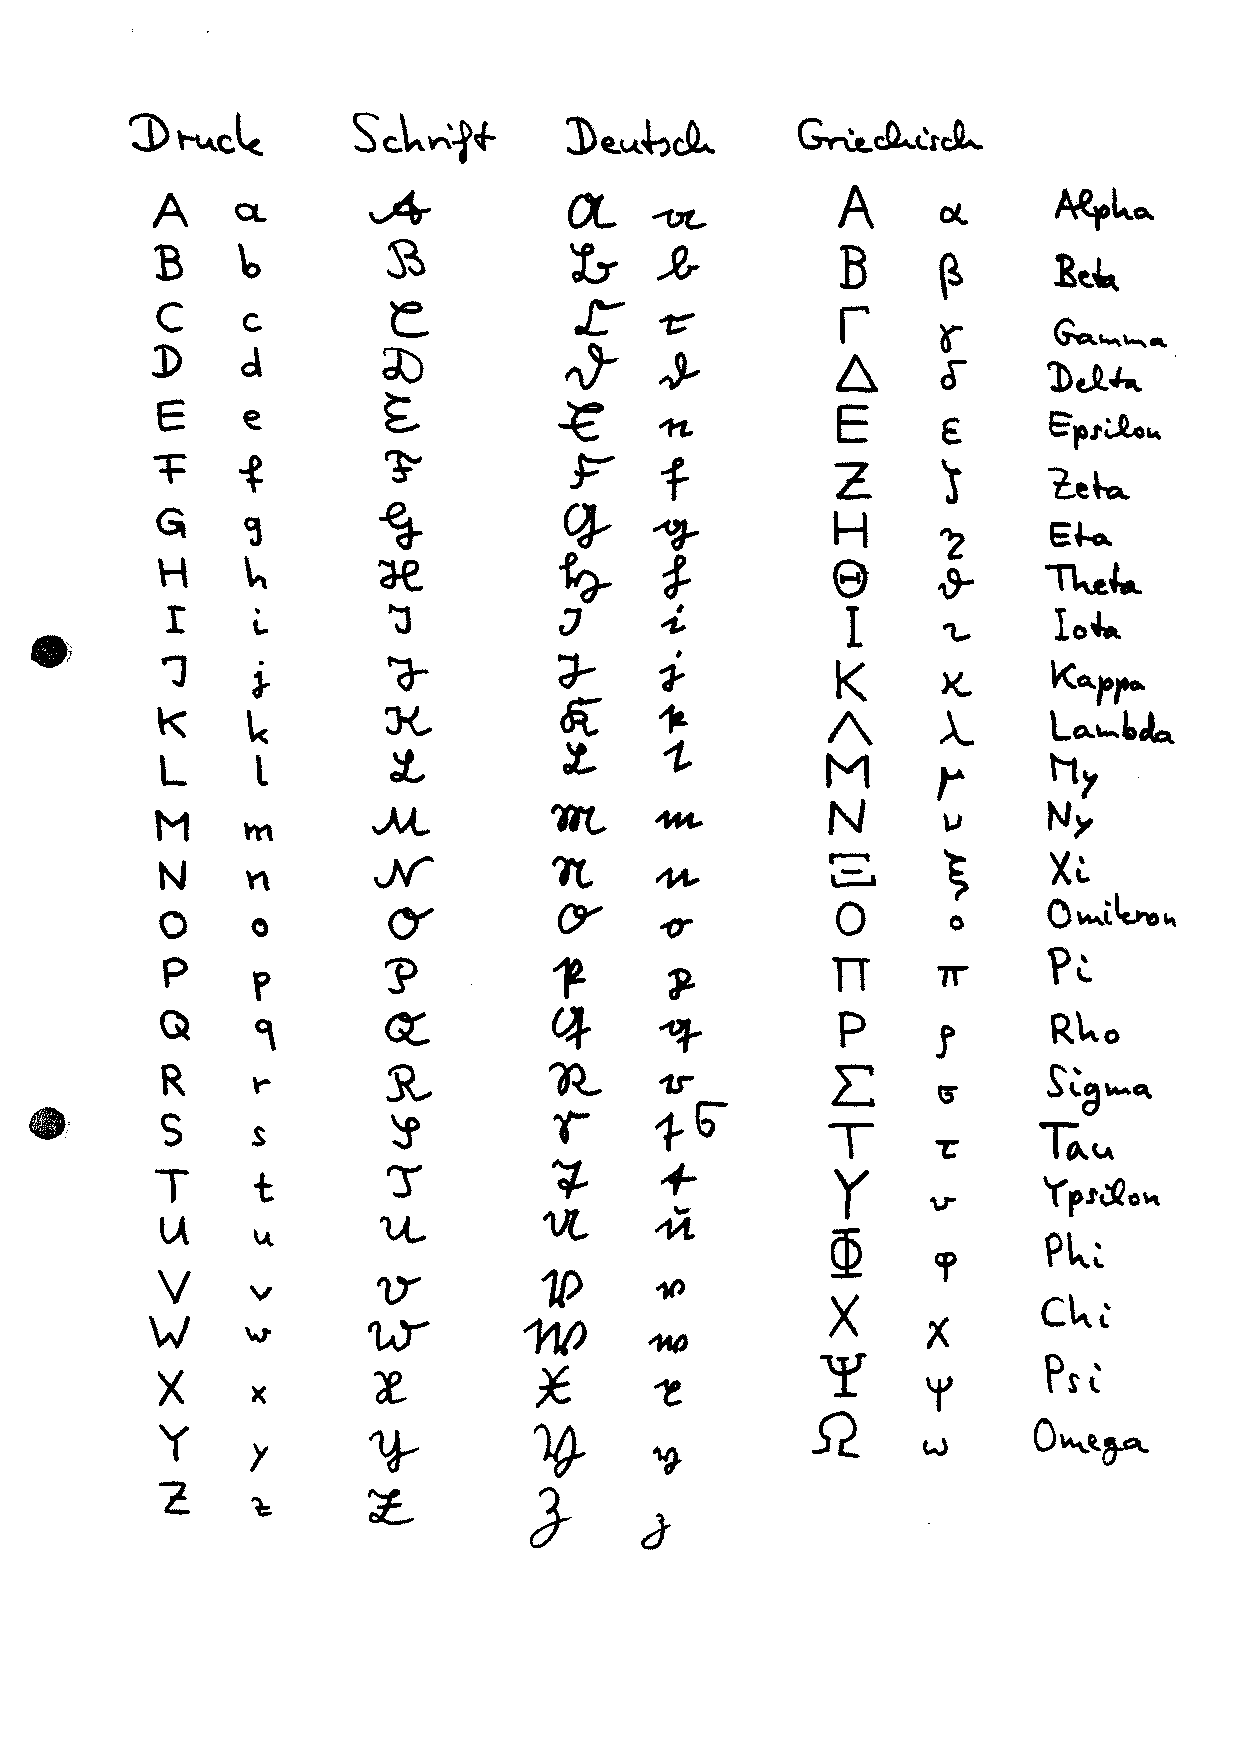
\includepdf[pages={1},addtotoc={1,section,1,Alphabete,alphabete}]{Alphabete}
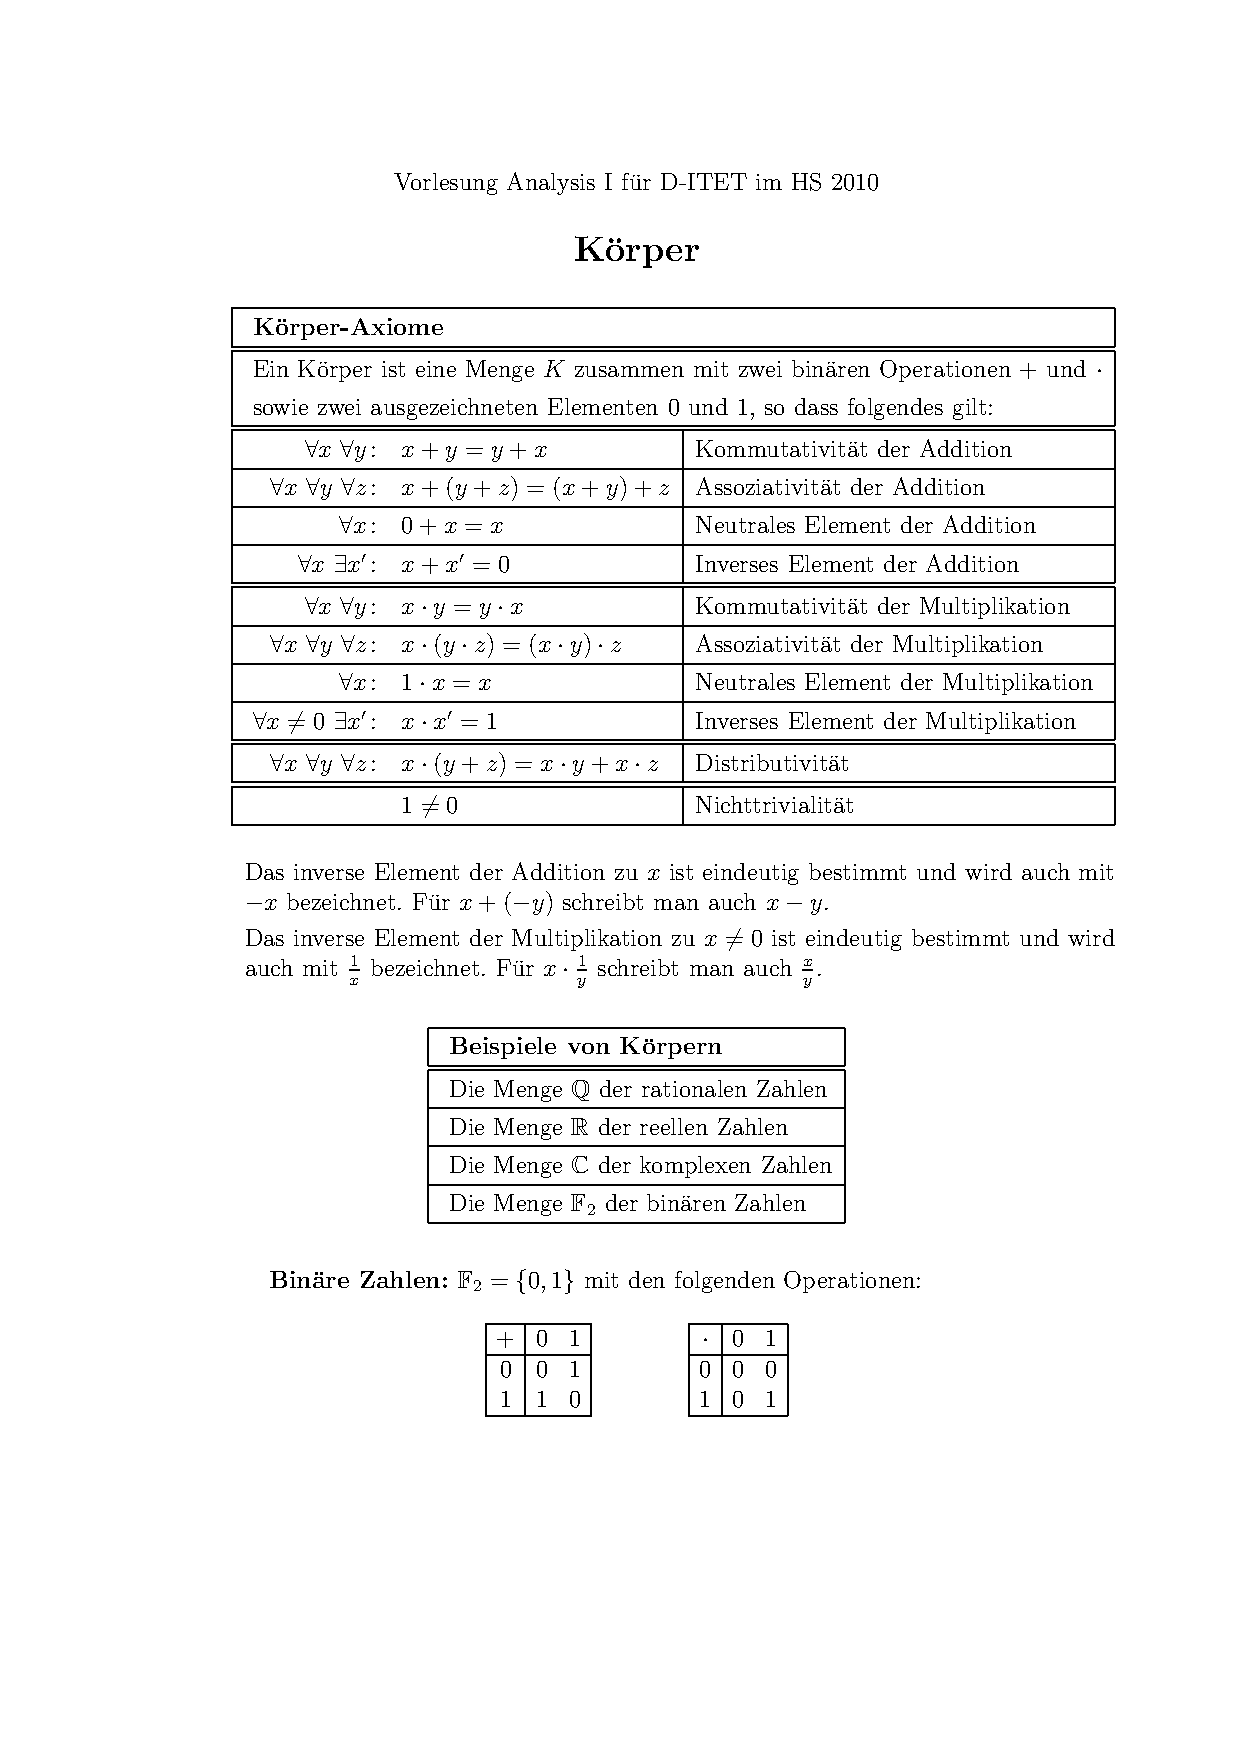
\includepdf[pages={1},addtotoc={1,section,1,Körper,koerper}]{Koerper}
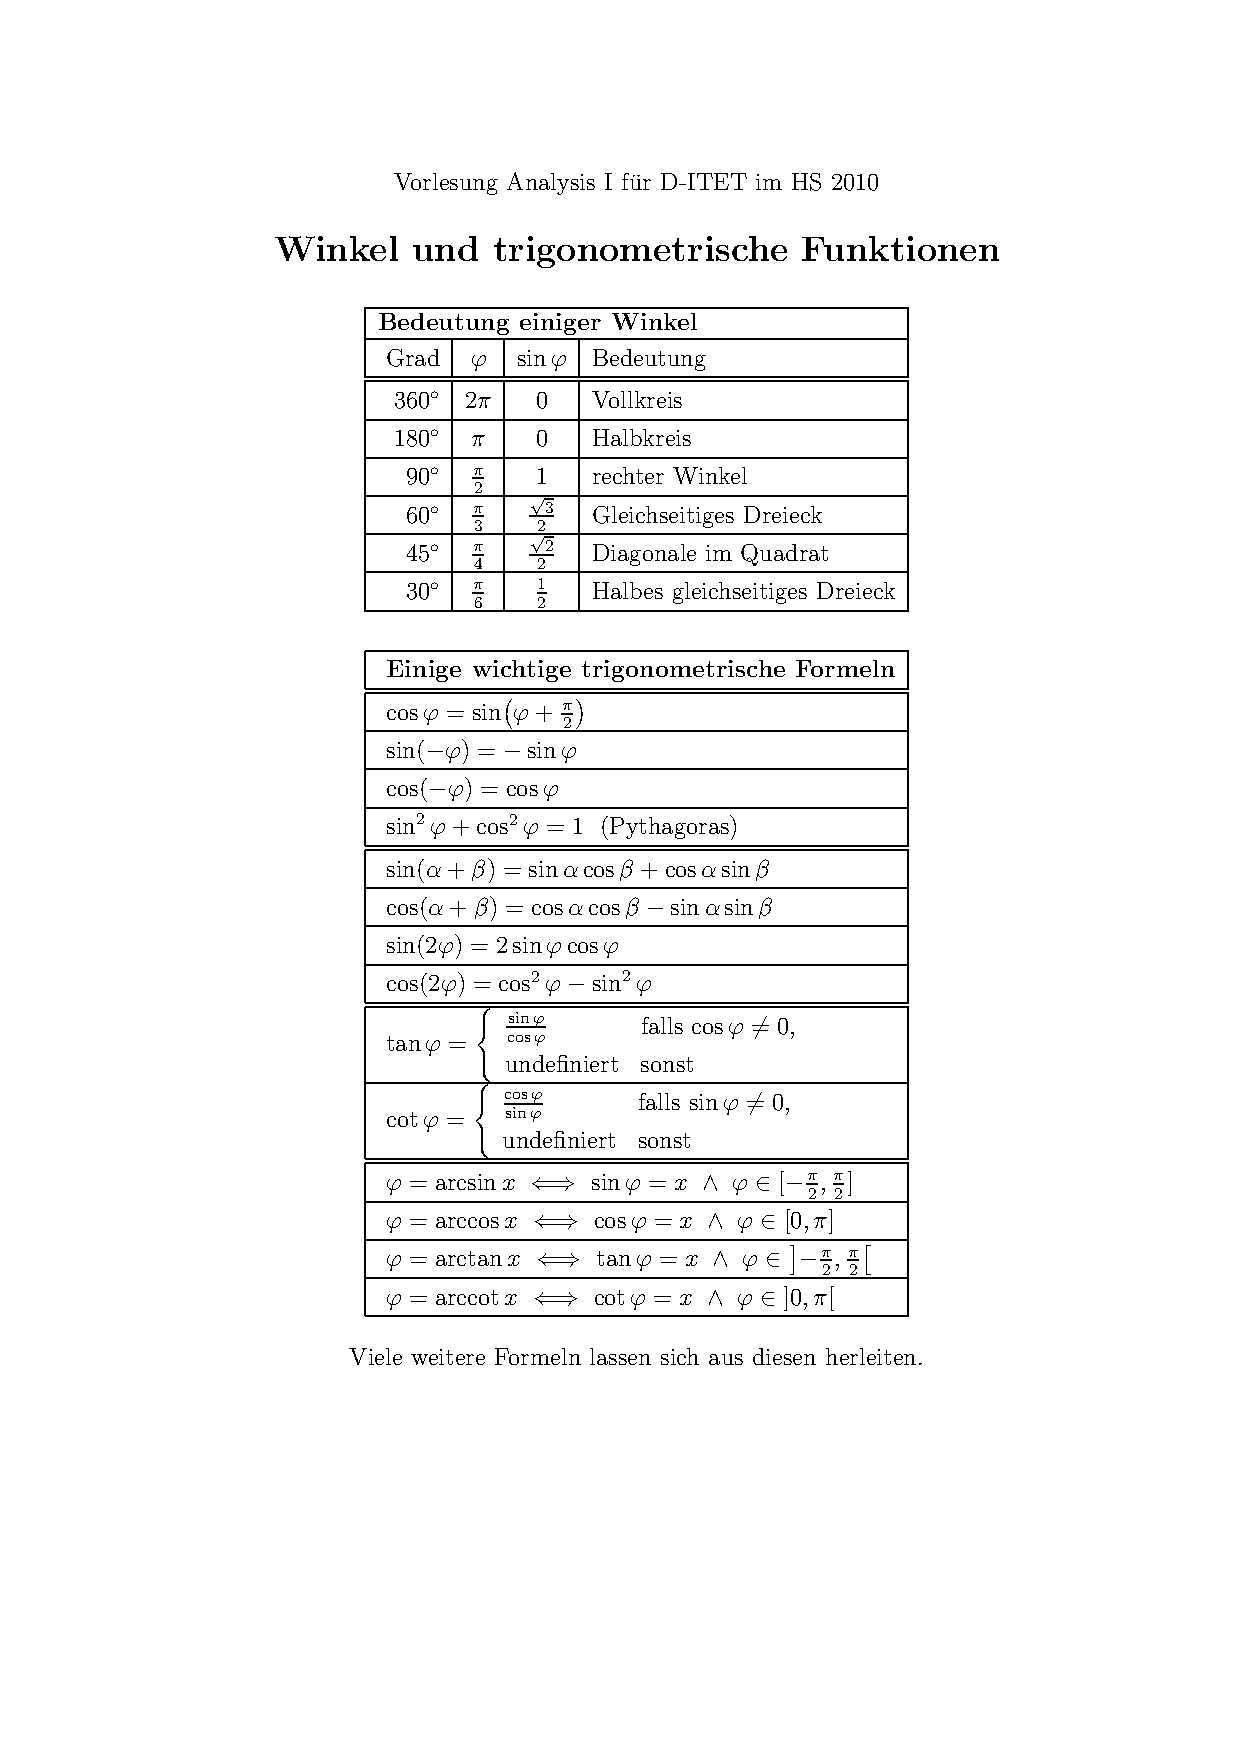
\includepdf[pages={1},addtotoc={1,section,1,Winkel und trigonometrische Frunktionen,trig}]{Trig}
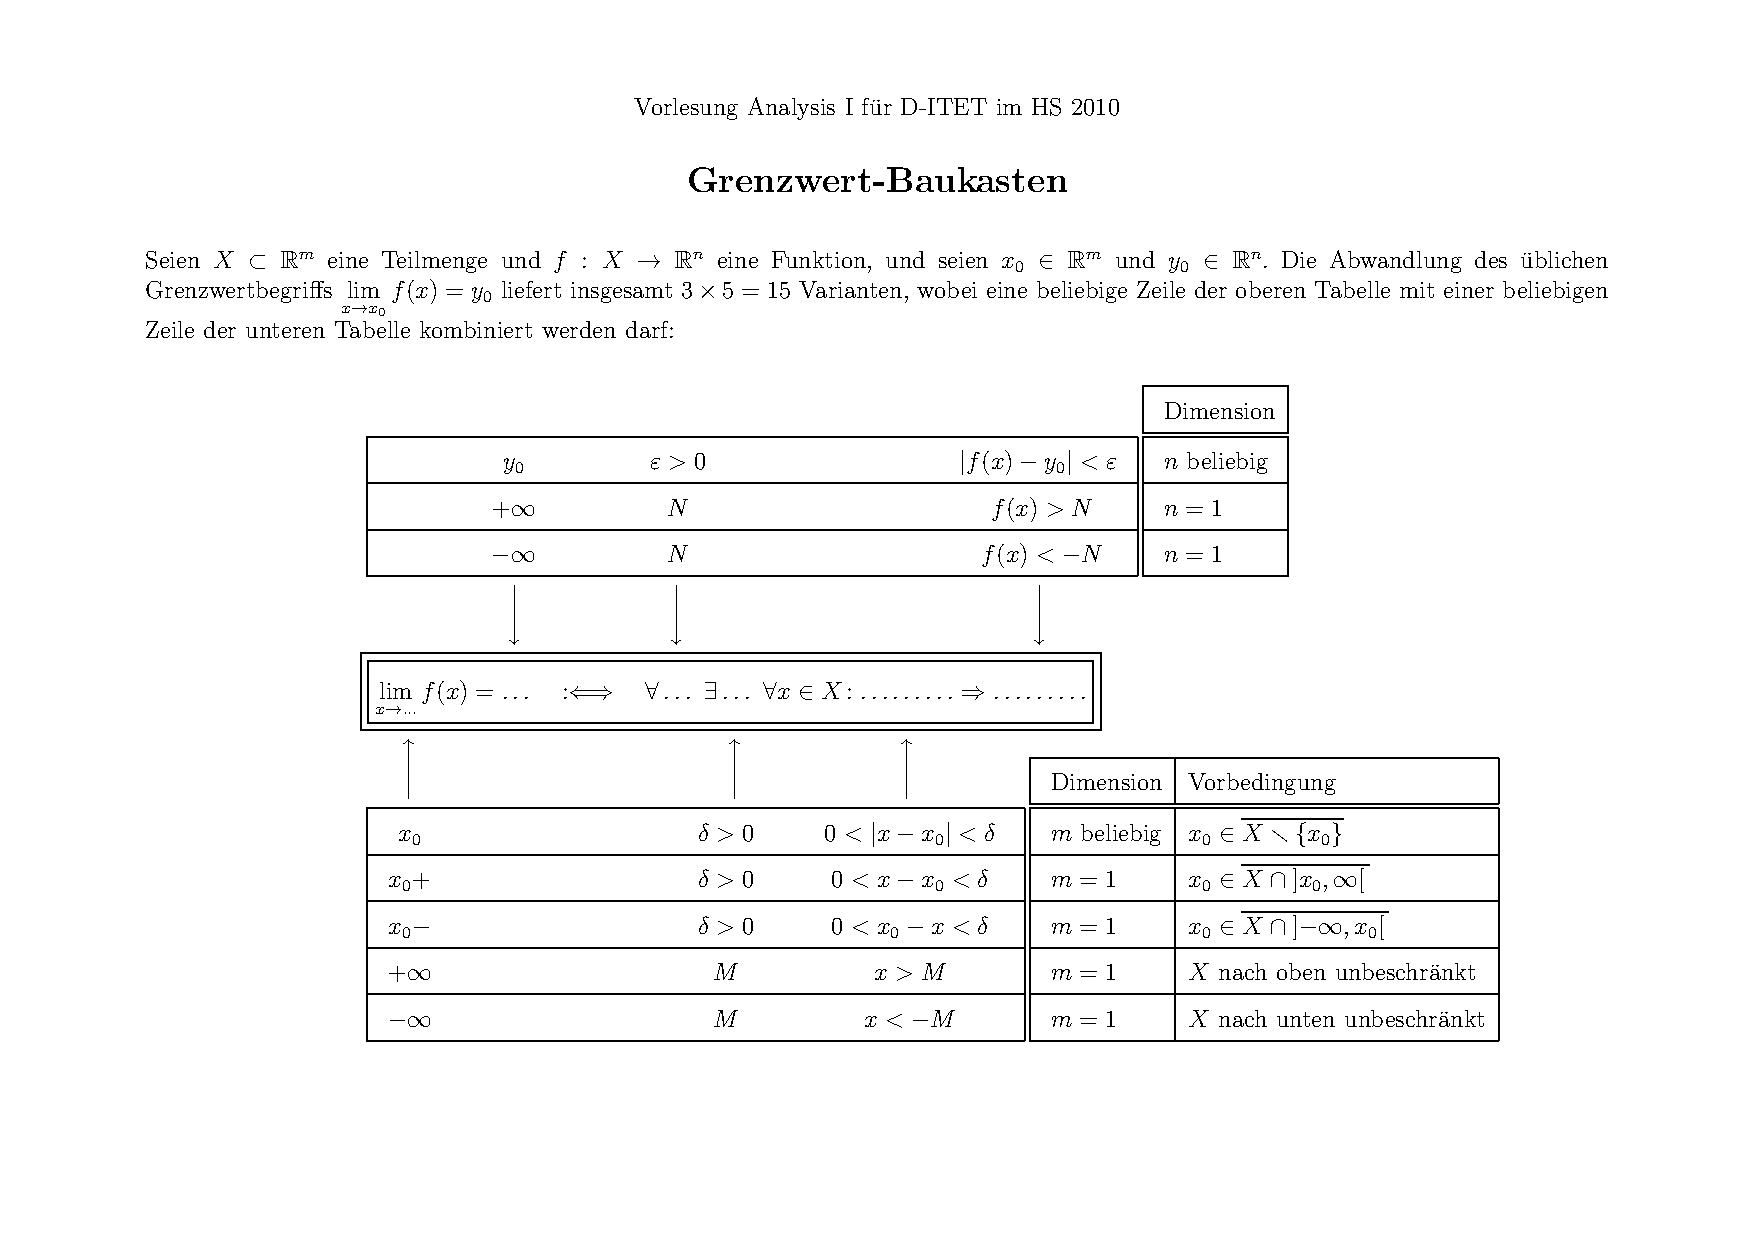
\includepdf[pages={1},addtotoc={1,section,1,Grenzwert-Baukasten,grenzwerte}]{Grenzwerte}
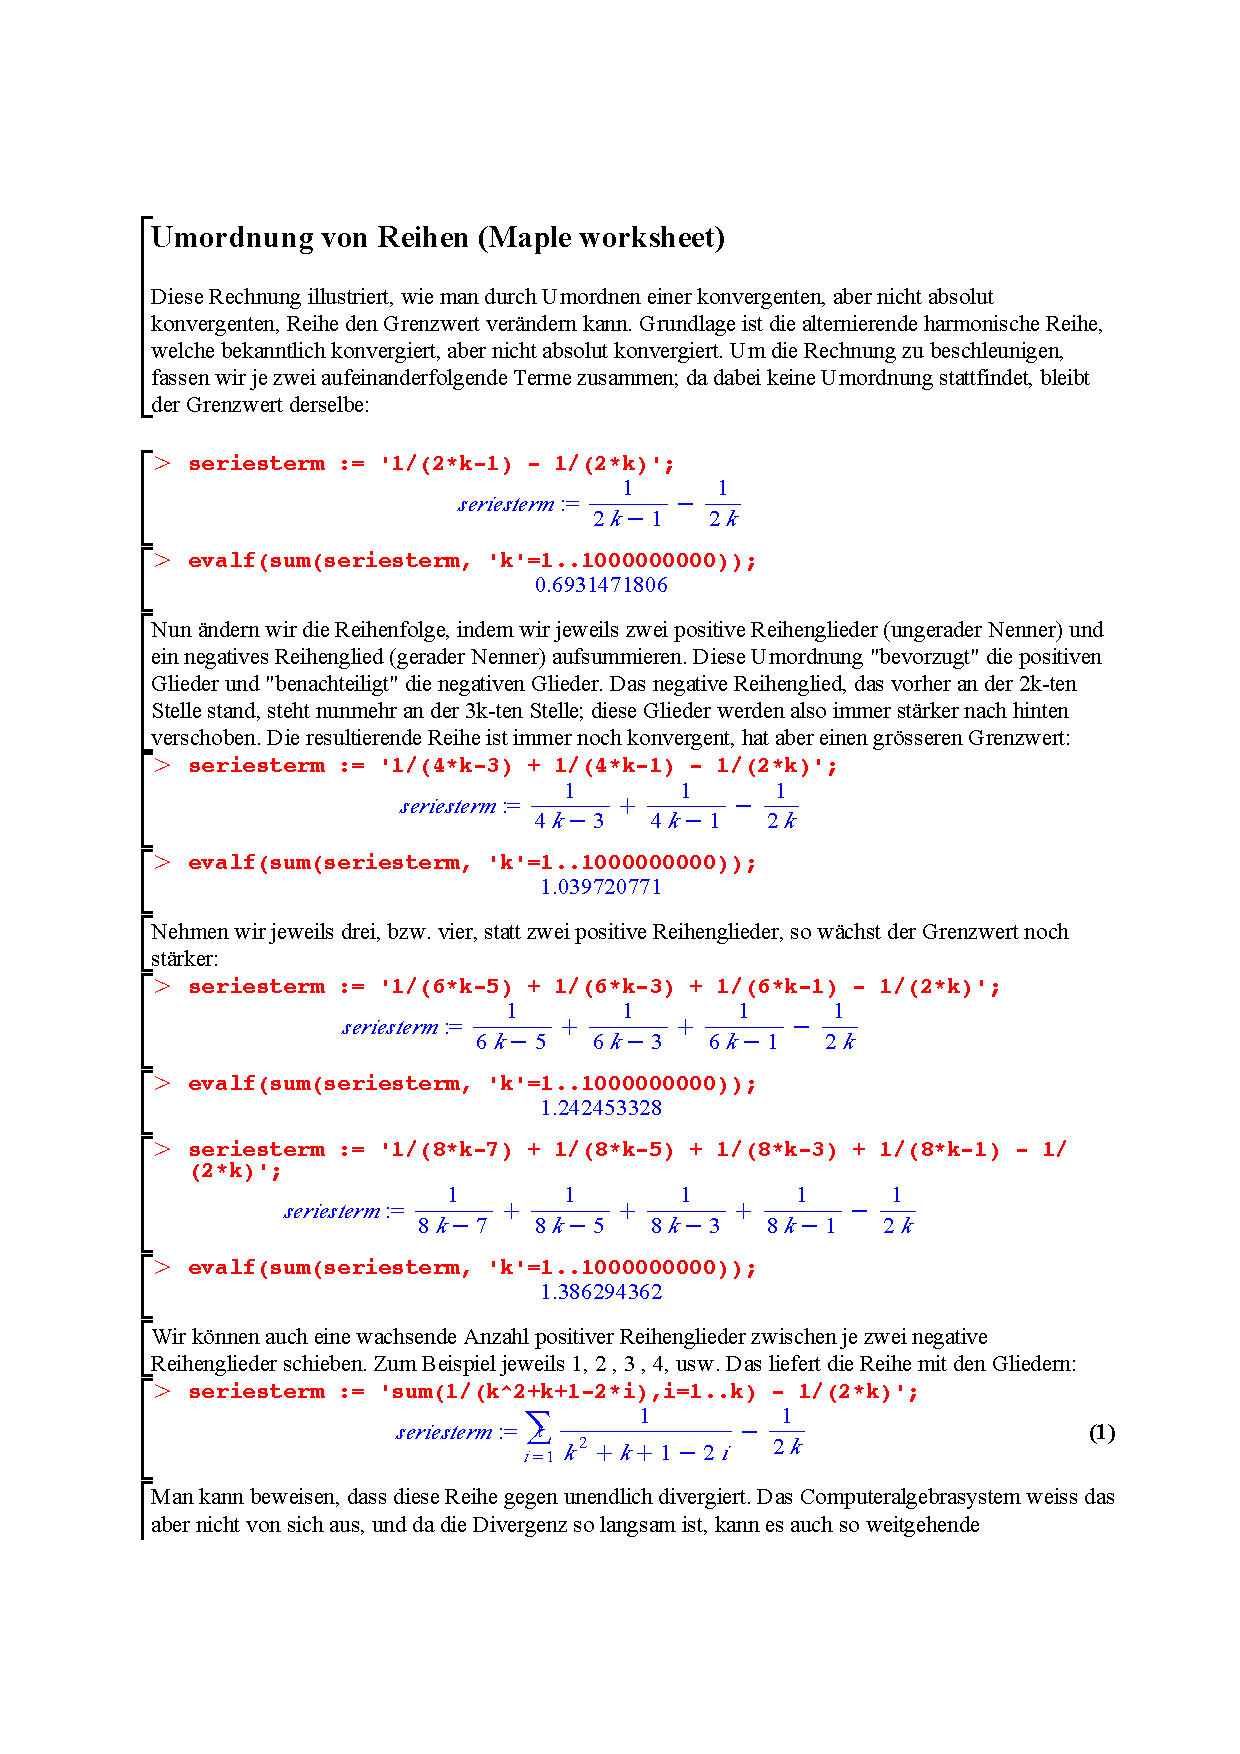
\includepdf[pages={1-2},addtotoc={1,section,1,Umordnung von Reihen,umodrnungreihen}]{Reihe-Umordnen}
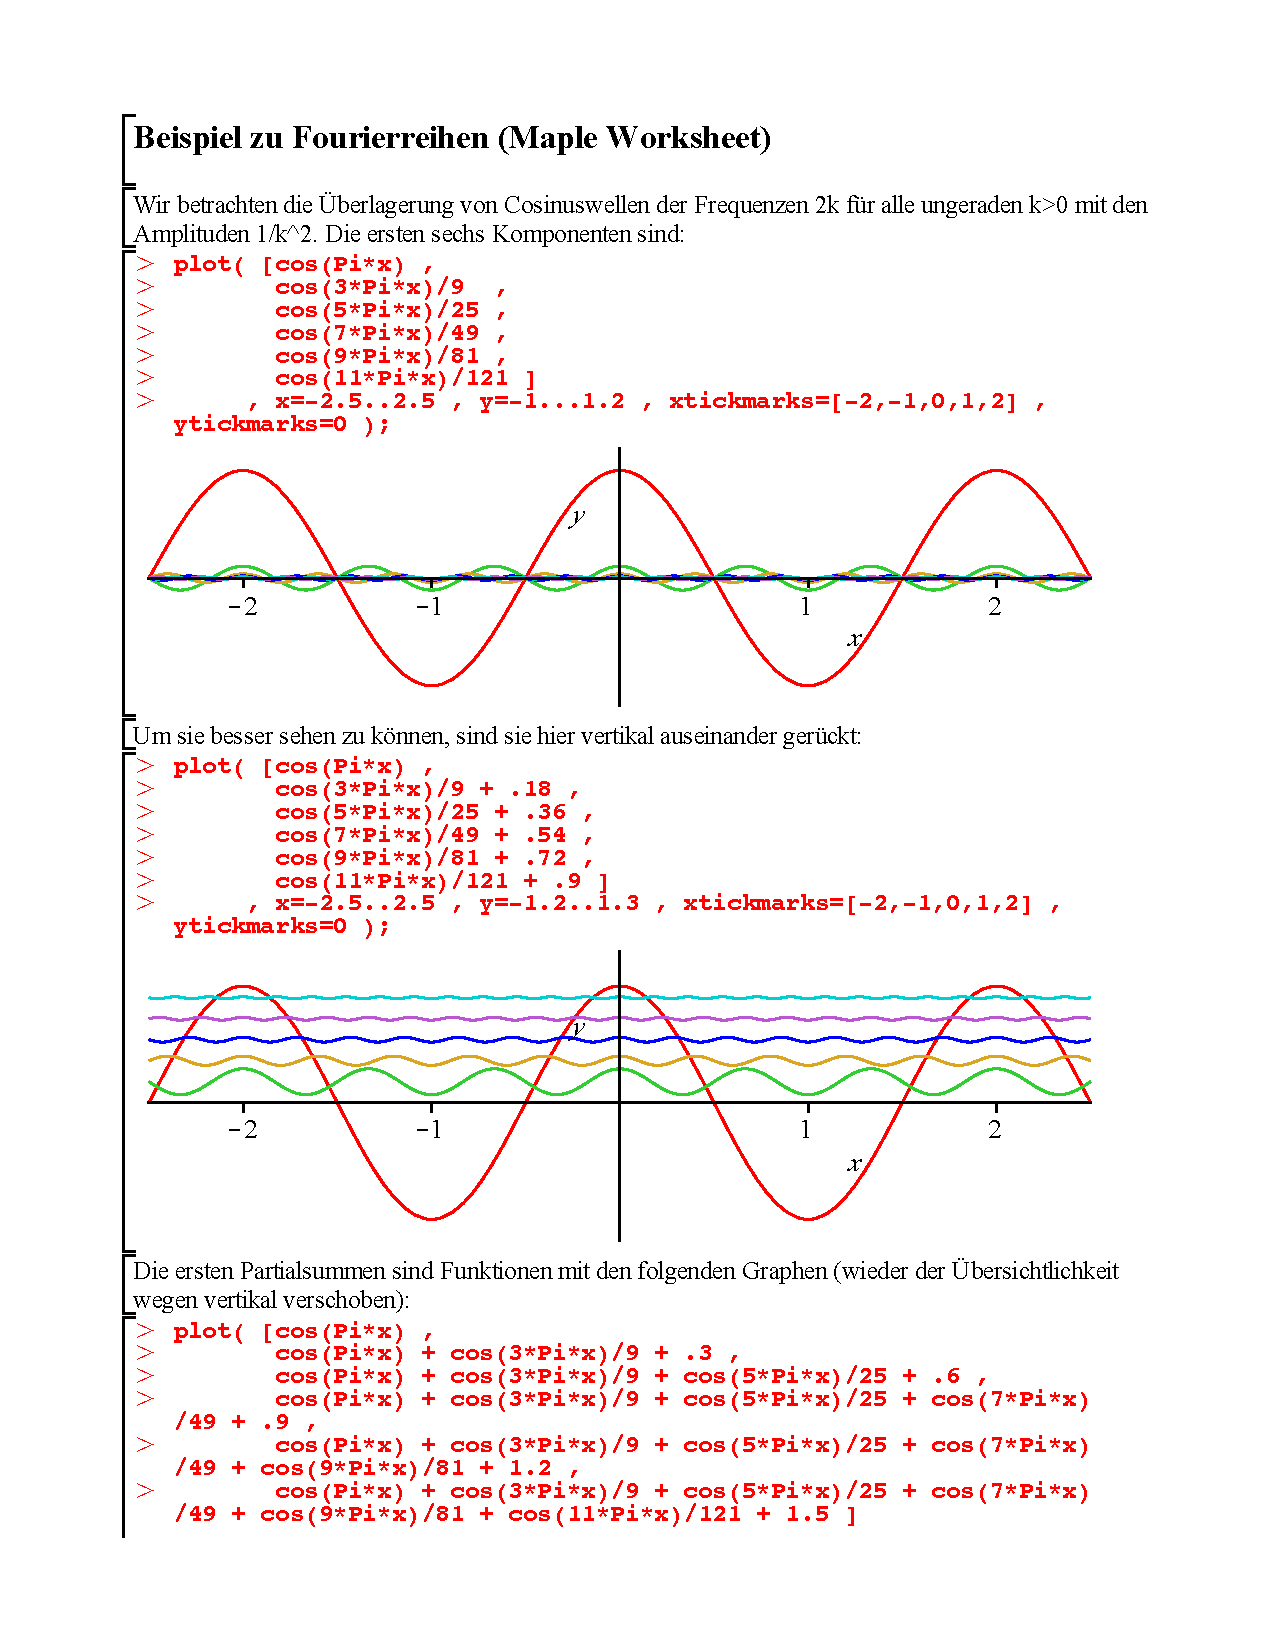
\includepdf[pages={1-3},addtotoc={1,section,1,Beispiel zu Fourierreihen,fourierbeispiel}]{Fourier-Beispiel}
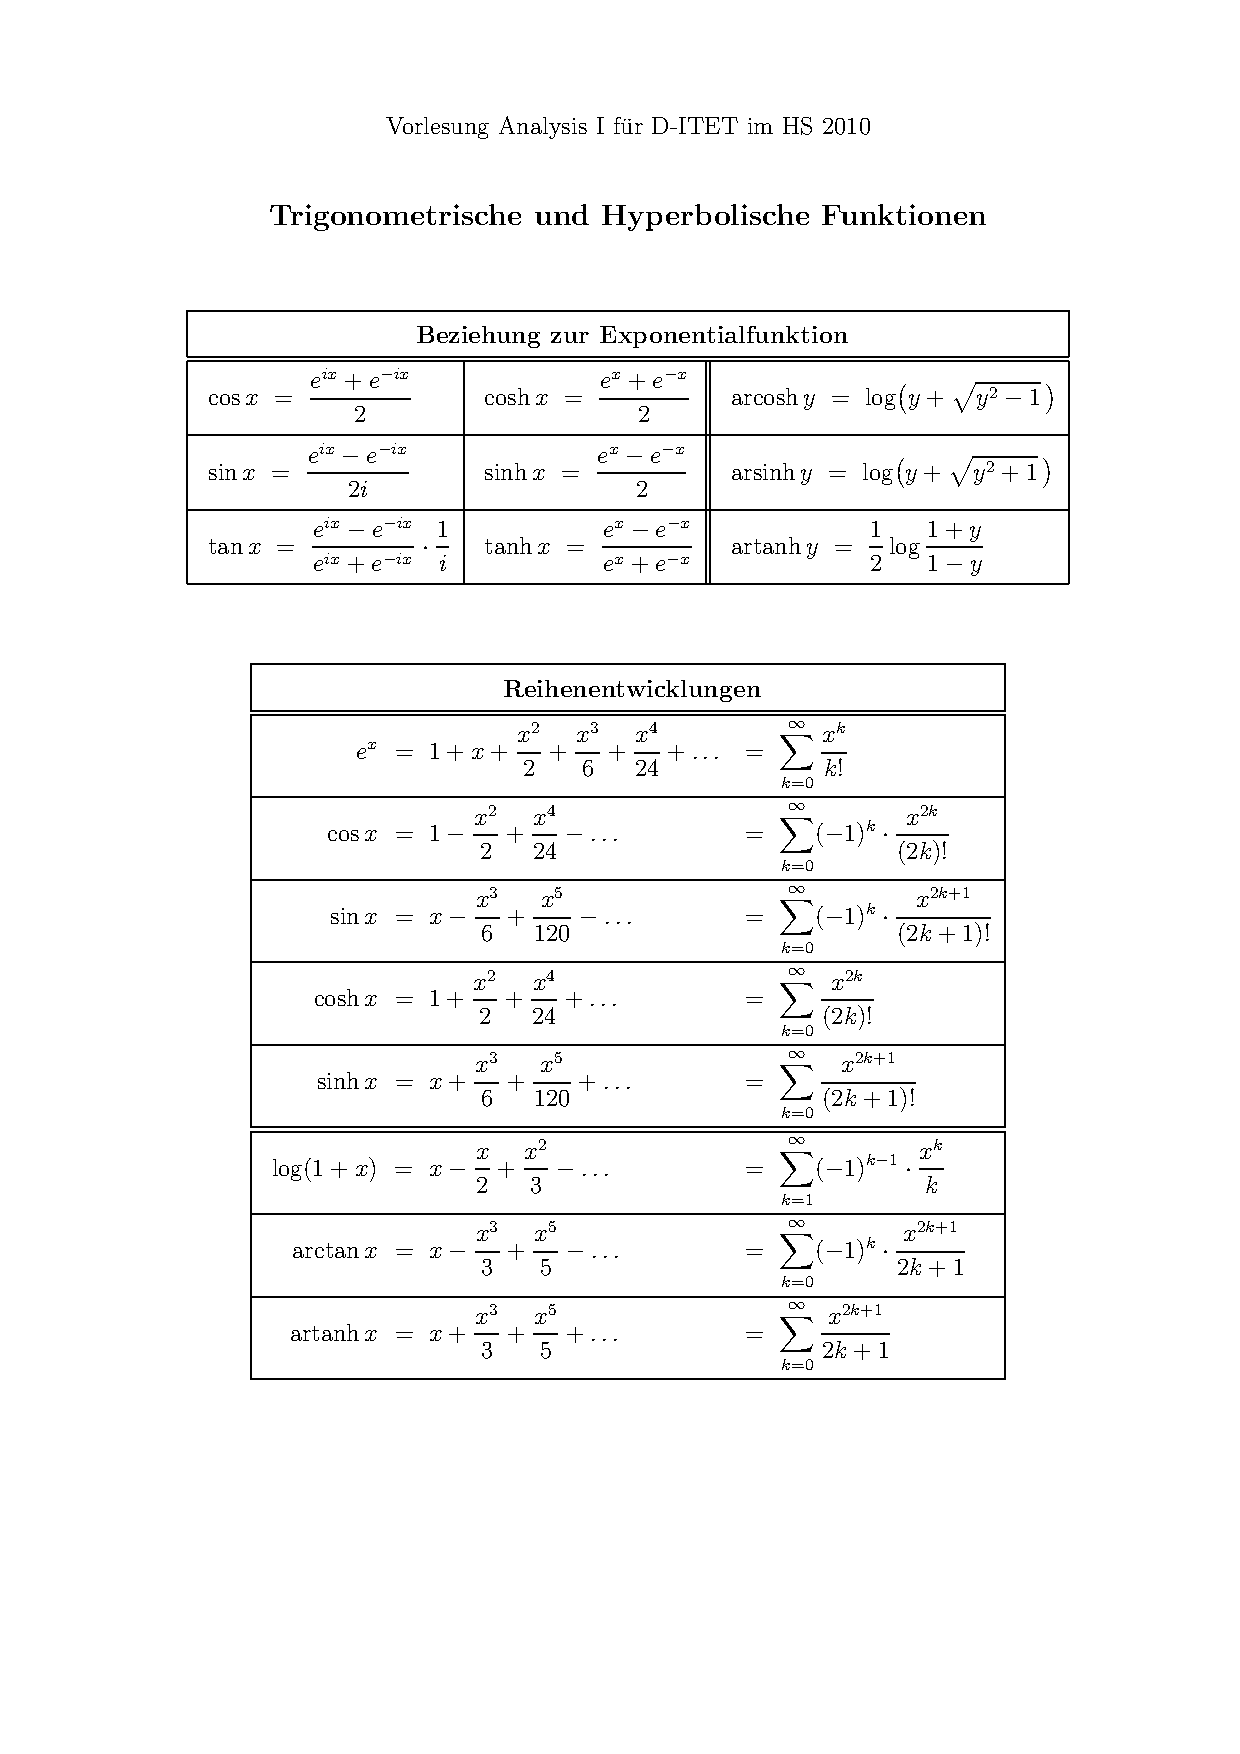
\includepdf[pages={1-2},addtotoc={1,section,1,Trigonometrische und Hyperbolische Funktionen,trighyp}]{TrigHyp}
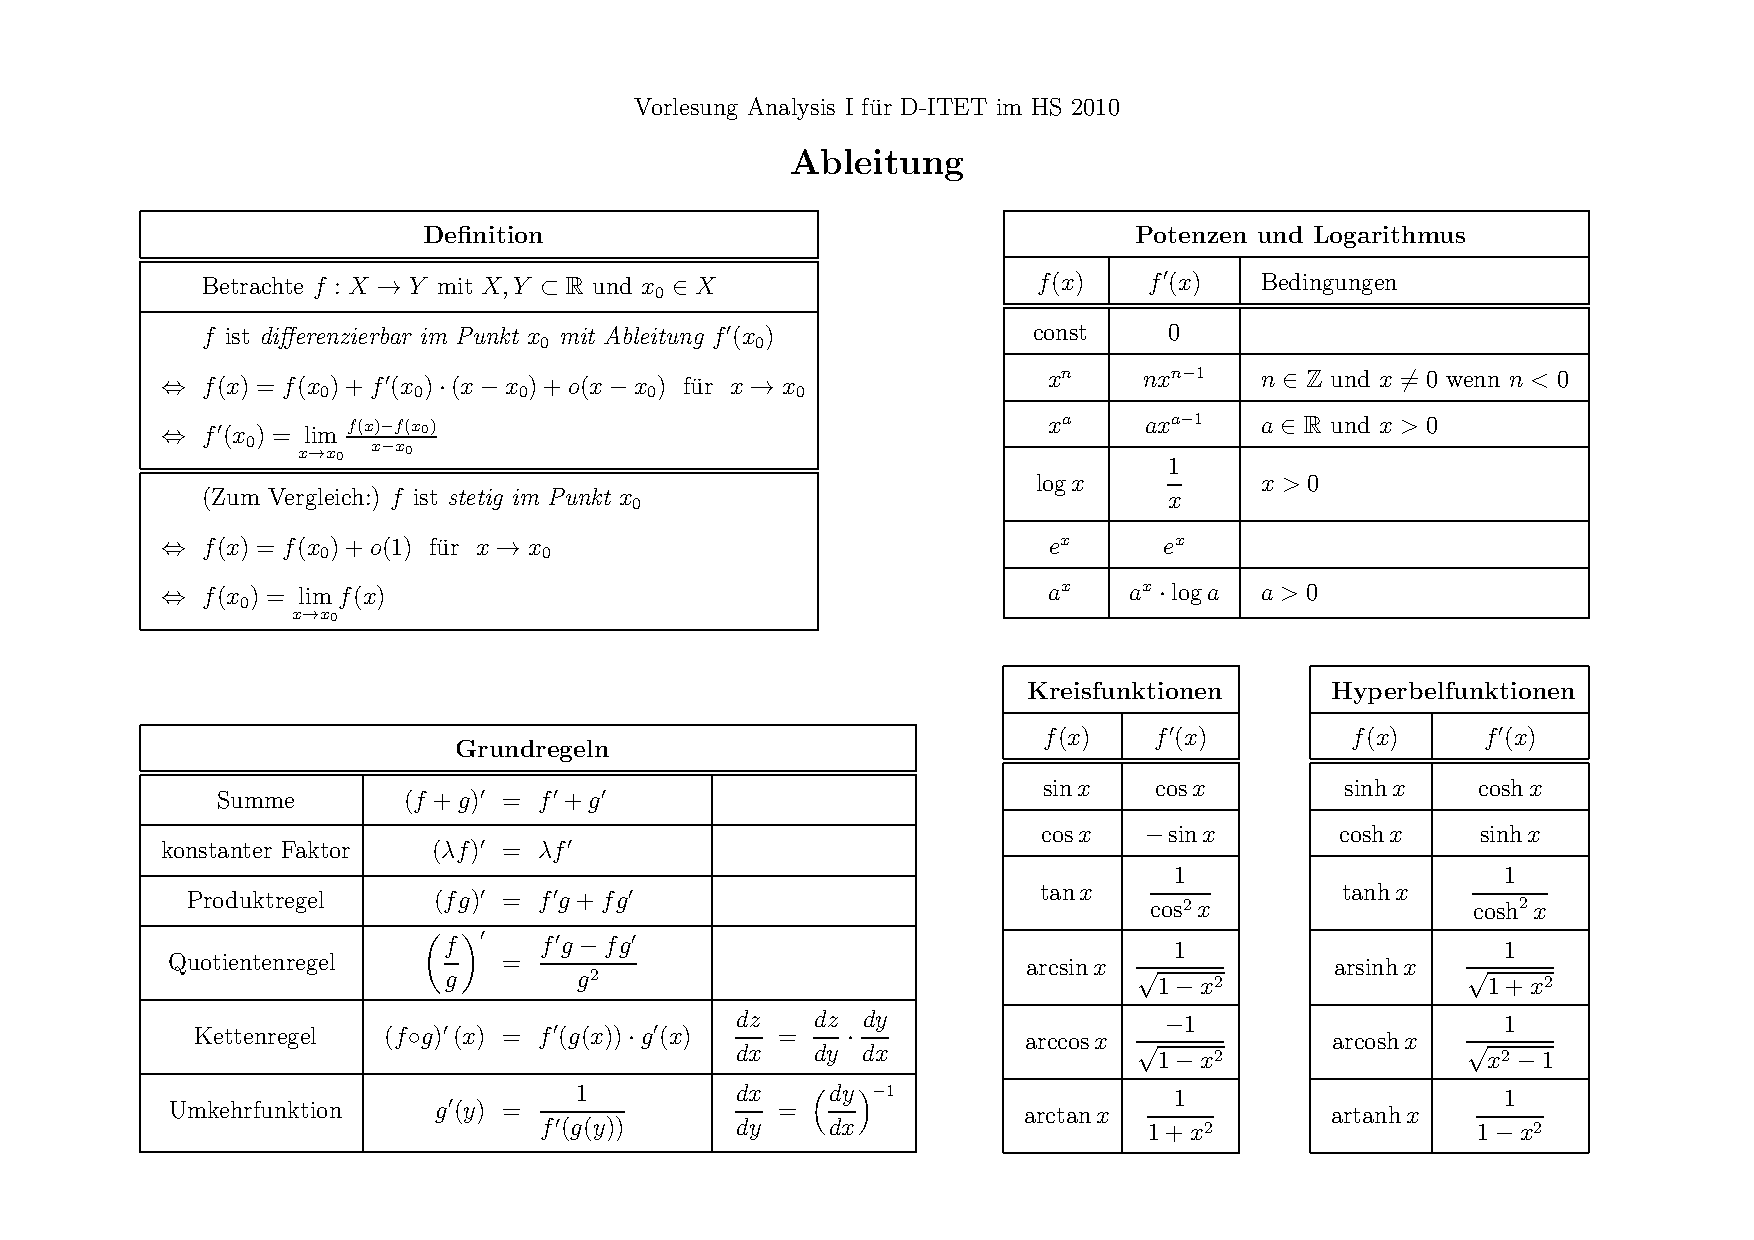
\includepdf[pages={1},addtotoc={1,section,1,Ableitungen,ableitungen}]{Ableitung}
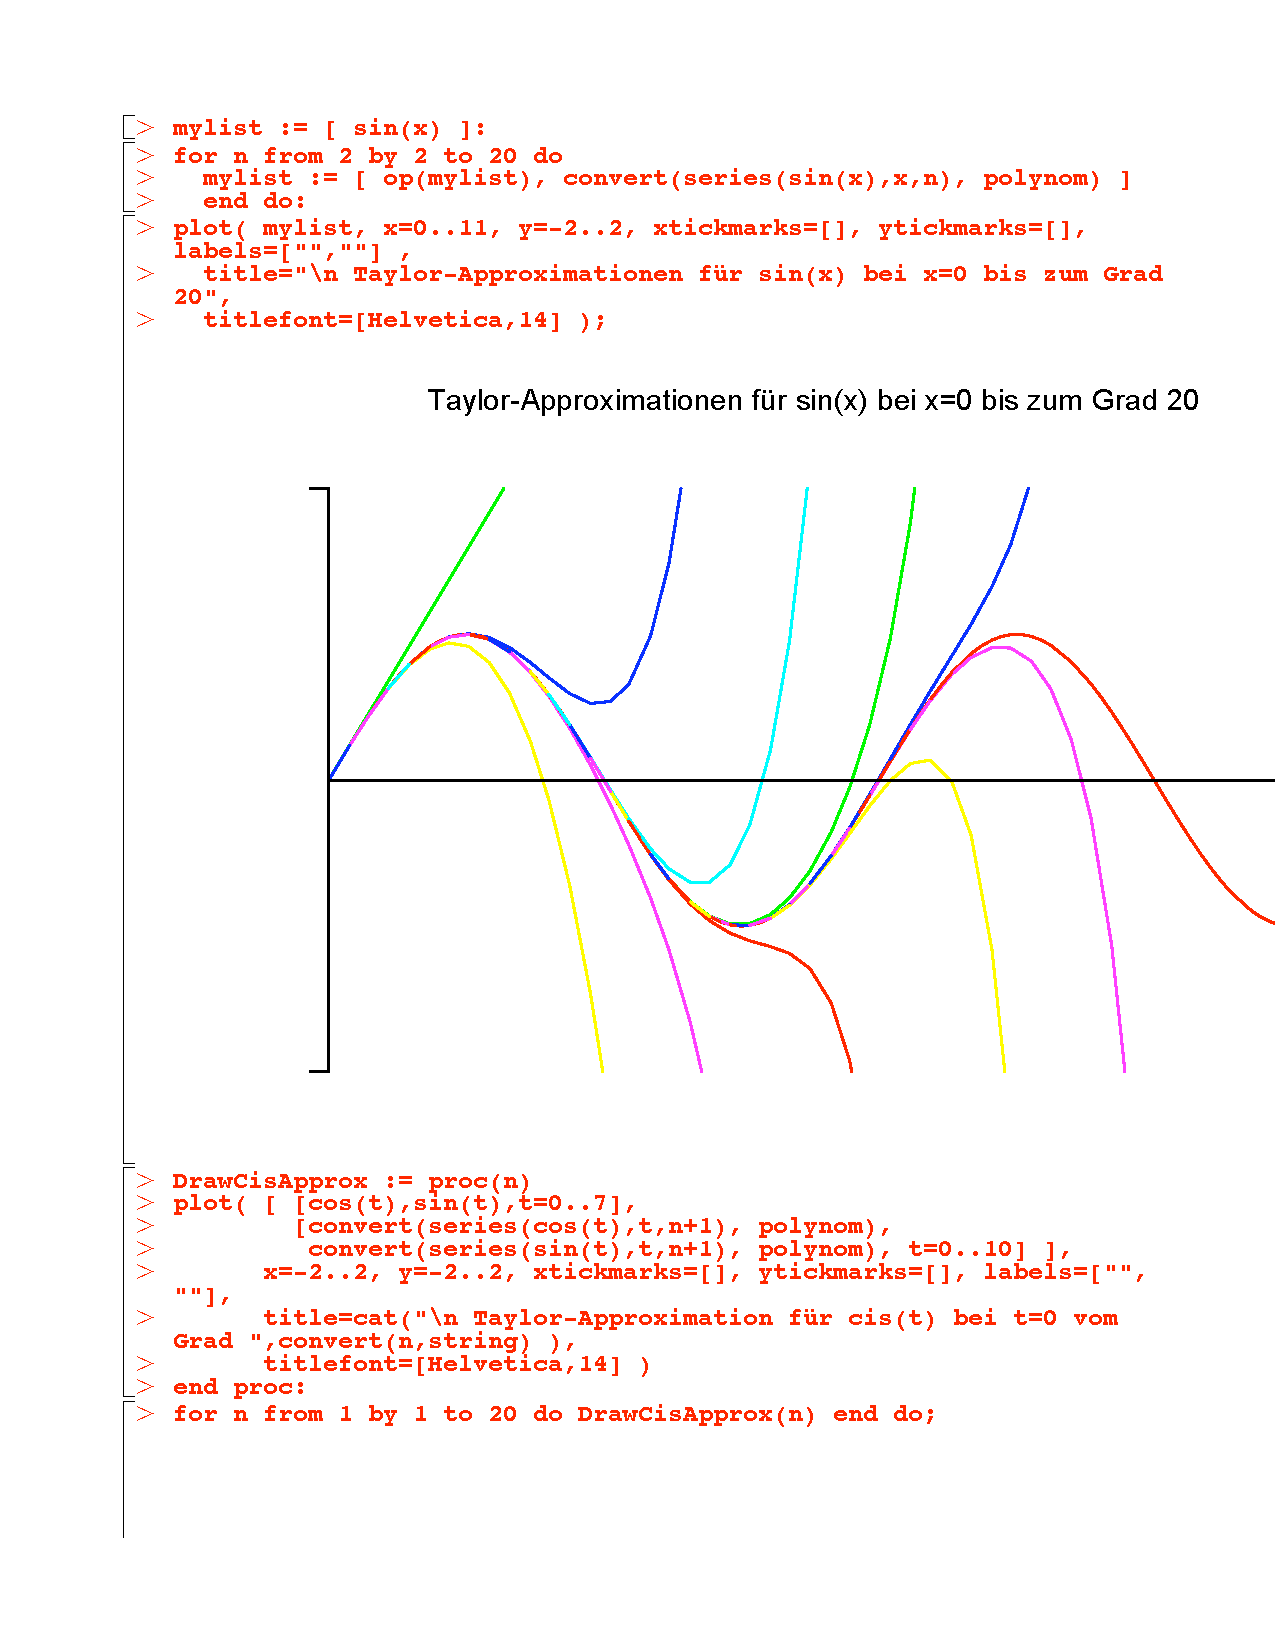
\includepdf[pages={1-21},addtotoc={1,section,1,Taylorapproximation der Funktionen sin und cis,taylorsincis}]{Taylor-Sin-Cis}
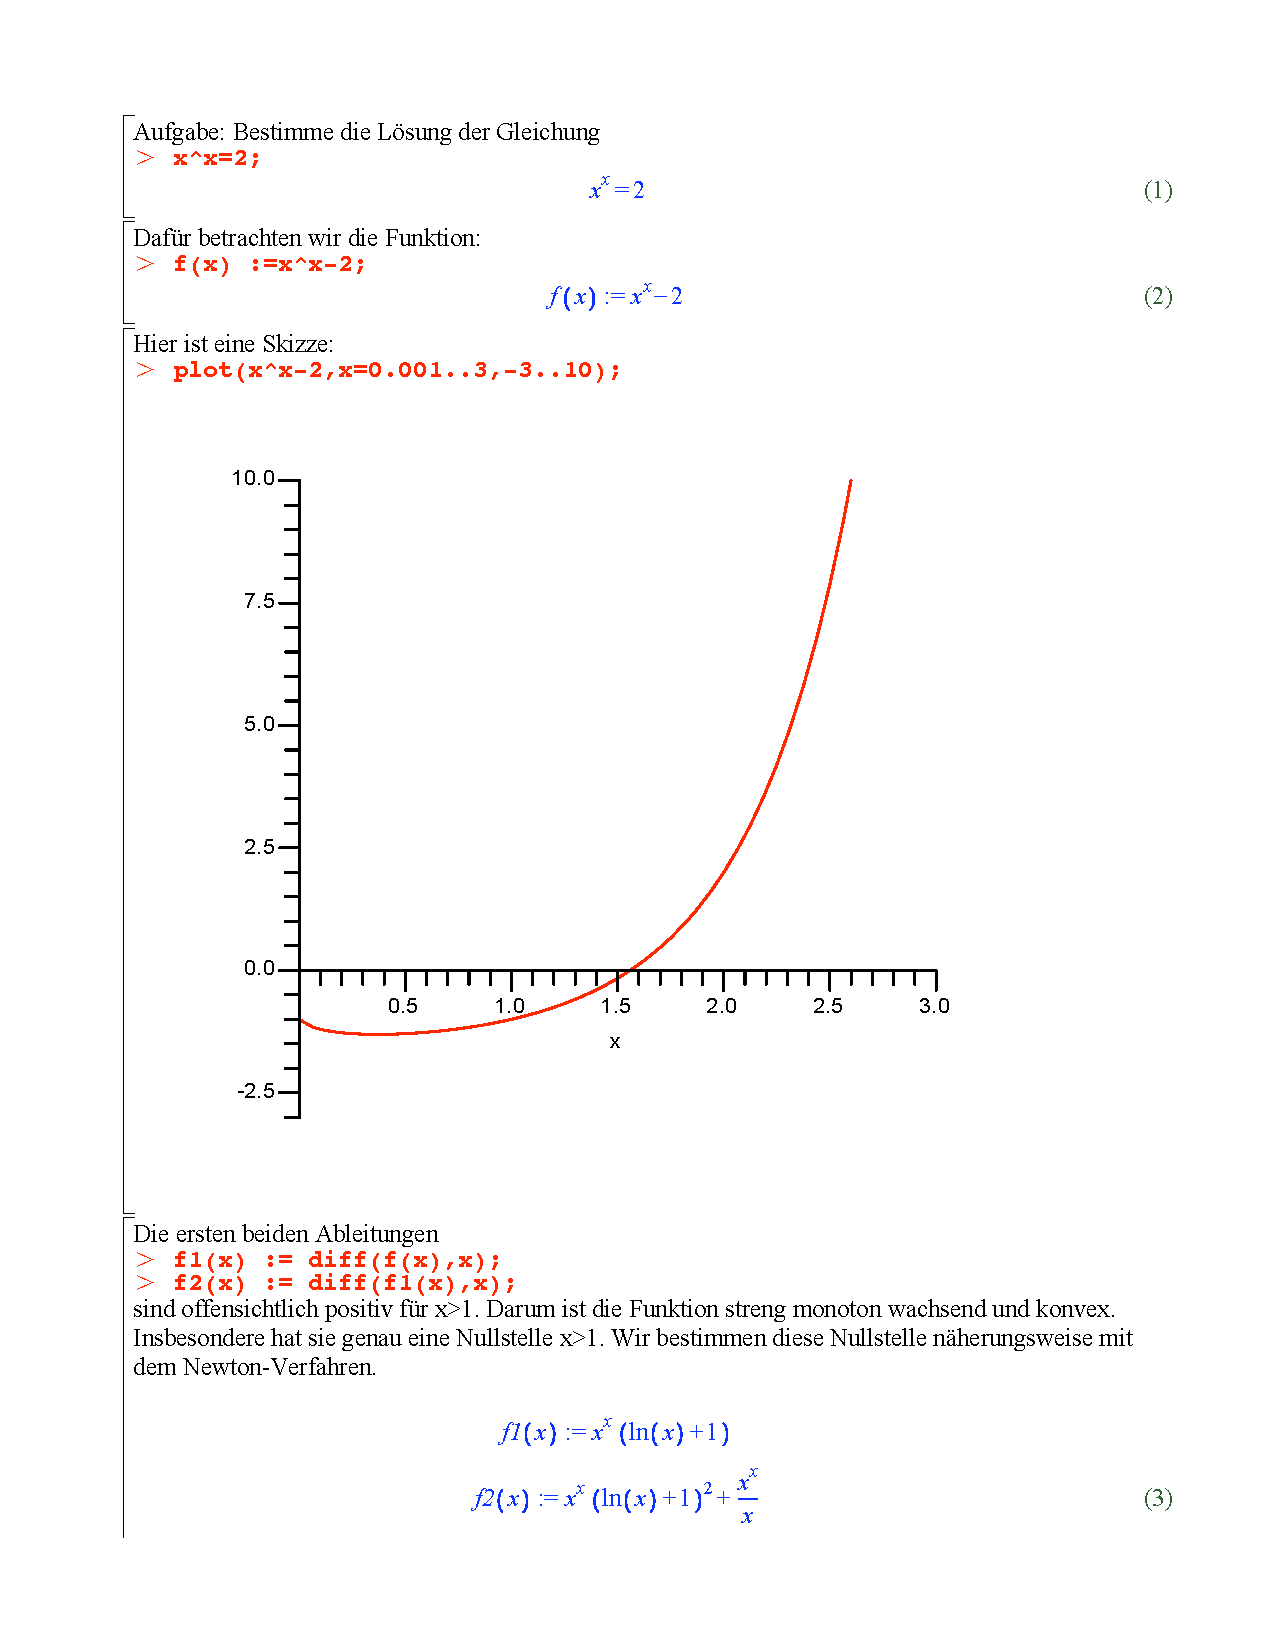
\includepdf[pages={1-11},addtotoc={1,section,1,Beispiel zum Newton-Verfahren,newton}]{Newton_xx2}
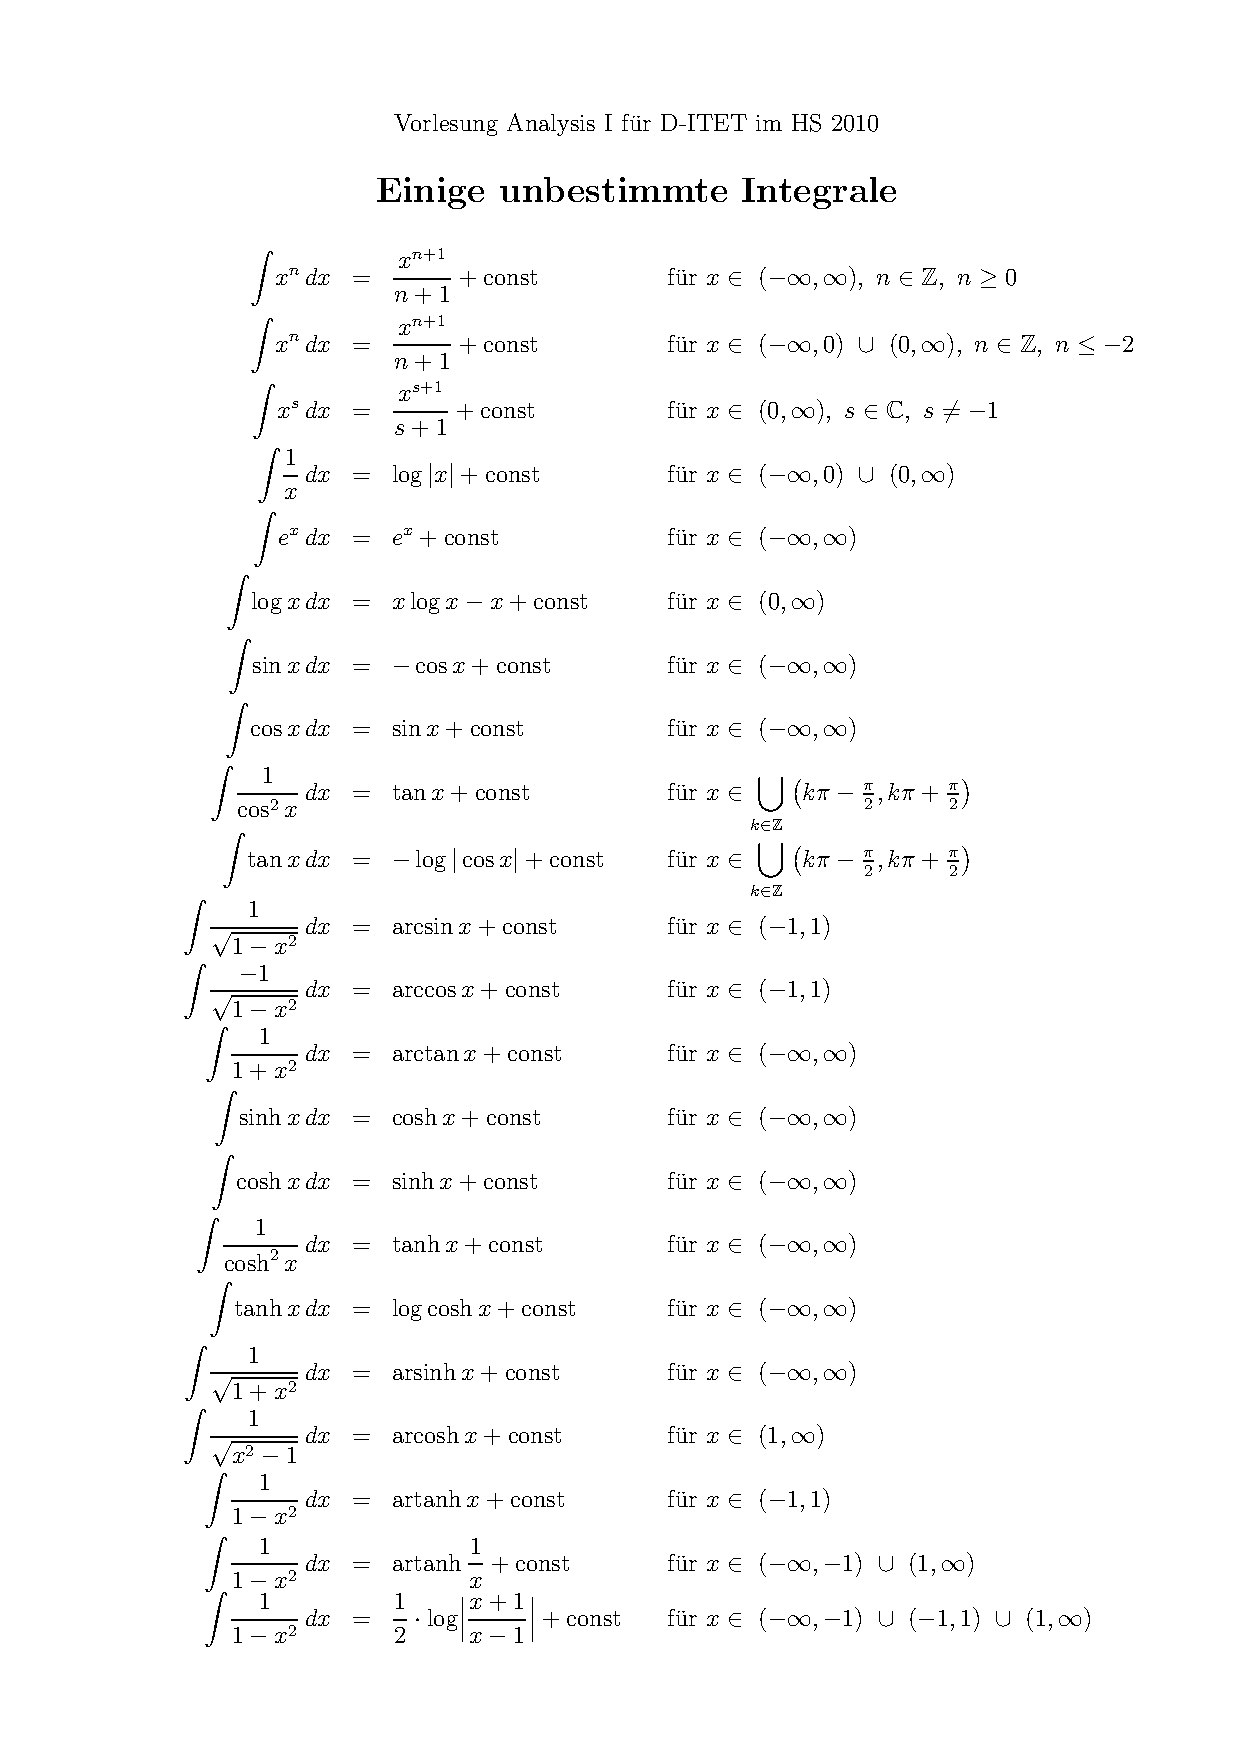
\includepdf[pages={1},addtotoc={1,section,1,Integralen,newton}]{Integralen}
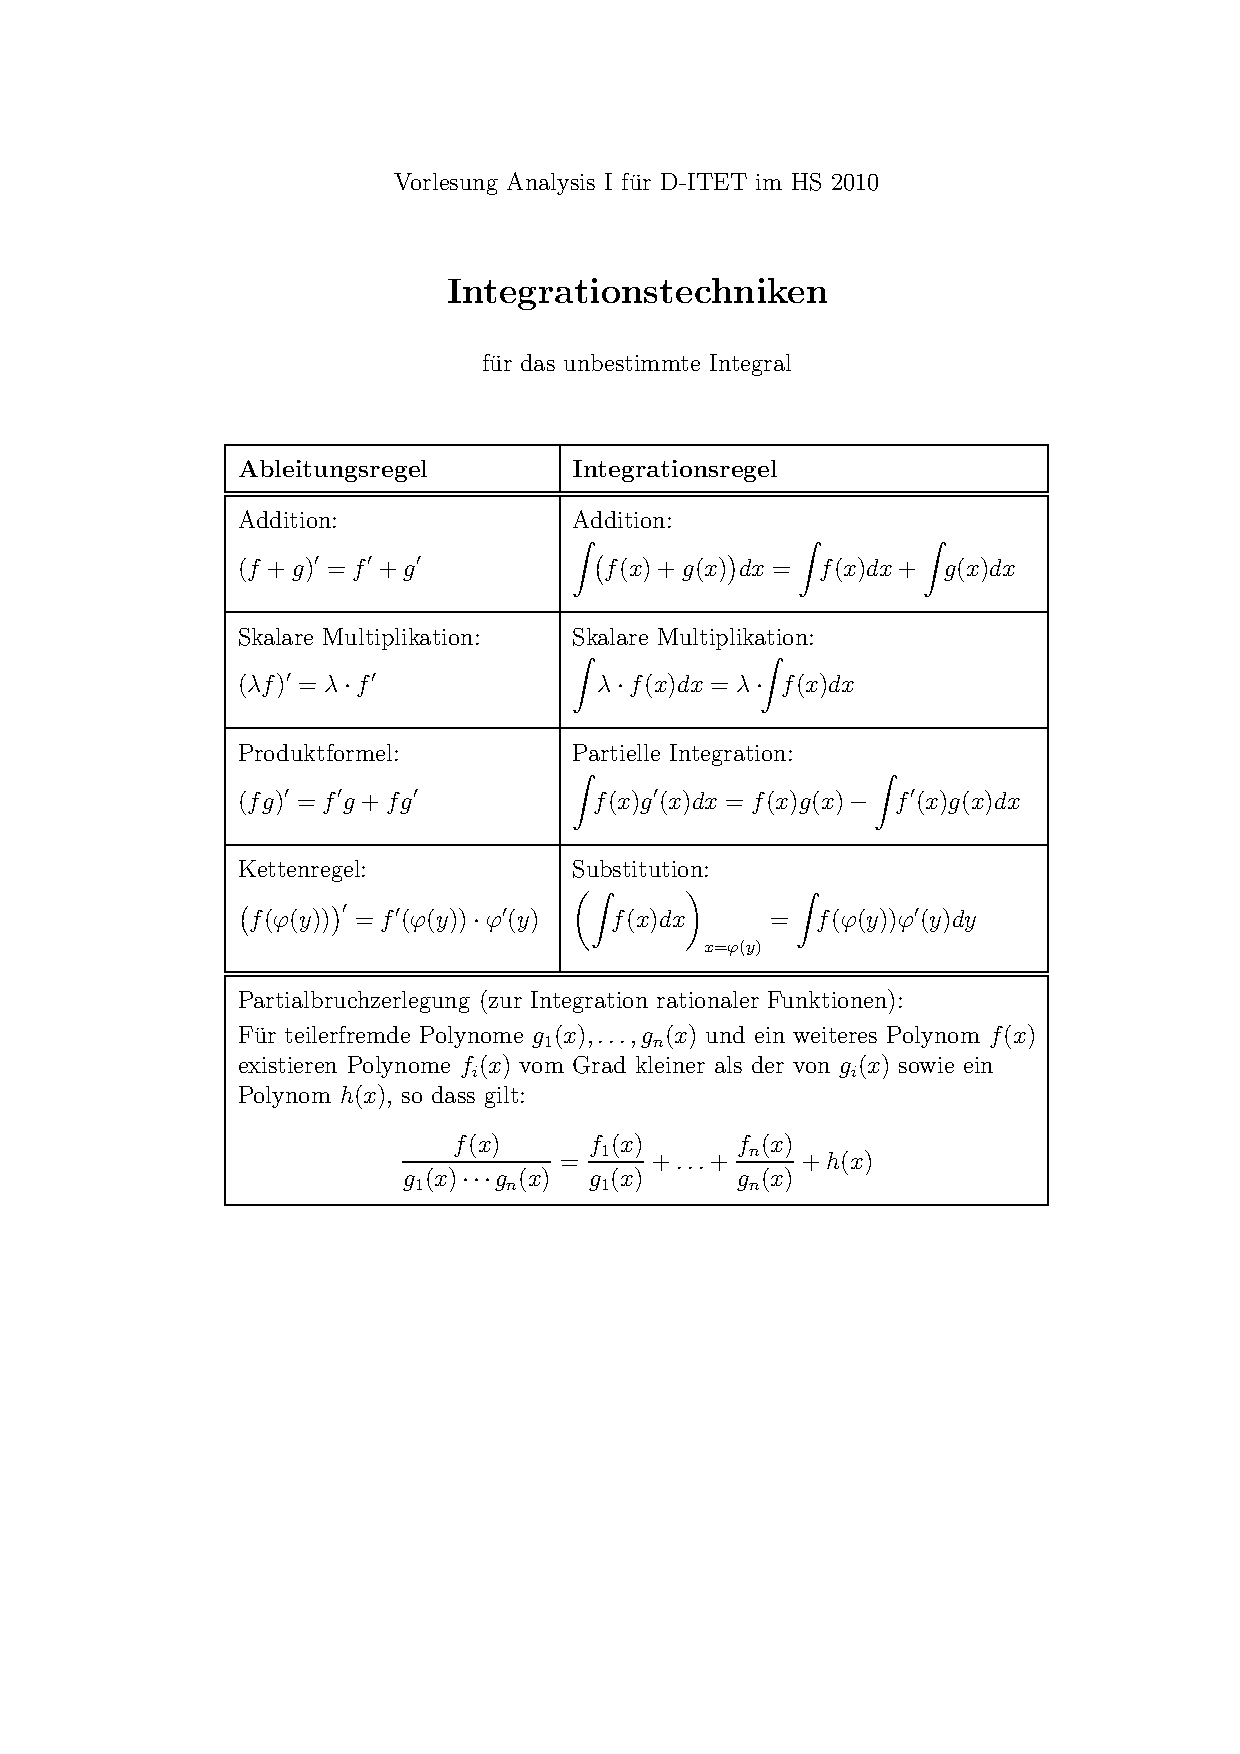
\includepdf[pages={1},addtotoc={1,section,1,Integrationstechniken,newton}]{Integrationstechniken}
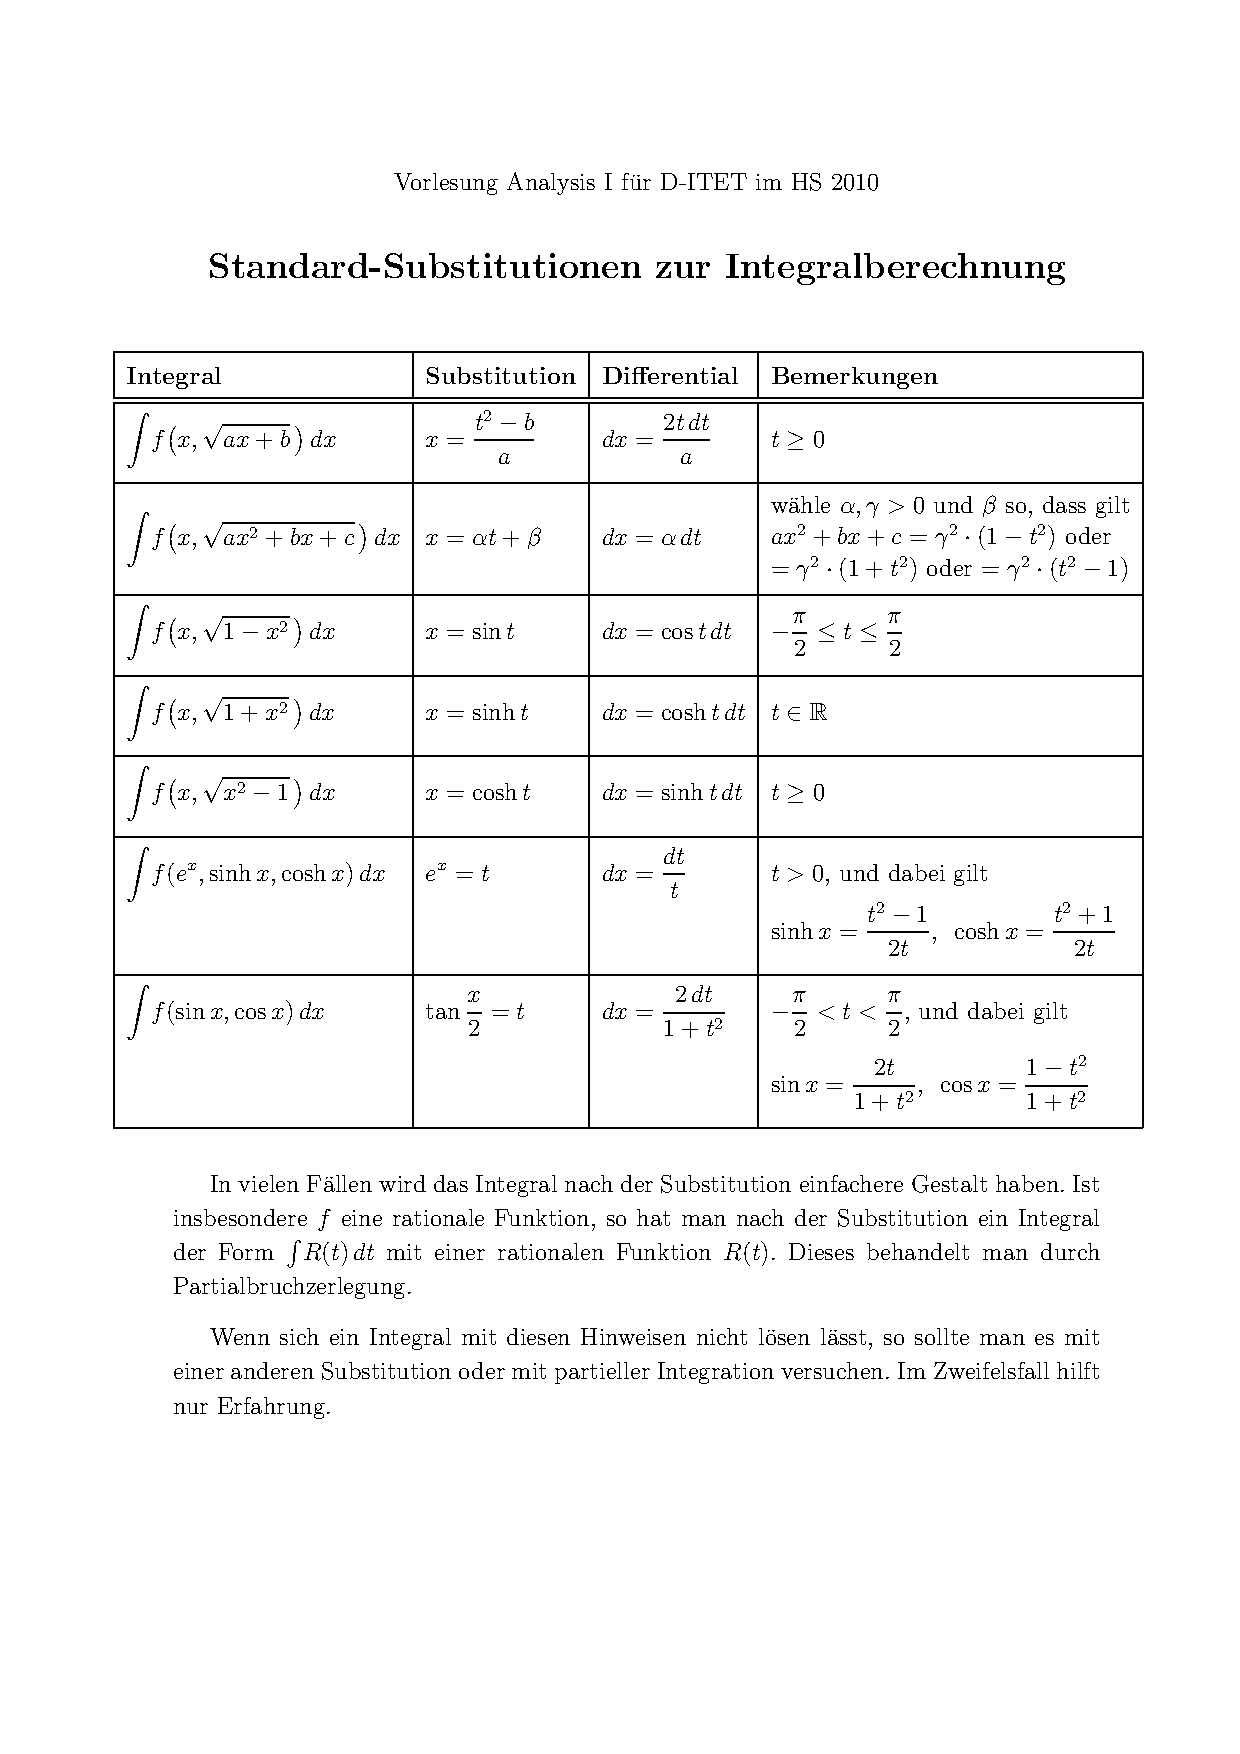
\includepdf[pages={1},addtotoc={1,section,1,Subtitutionen,newton}]{Substitutionen}
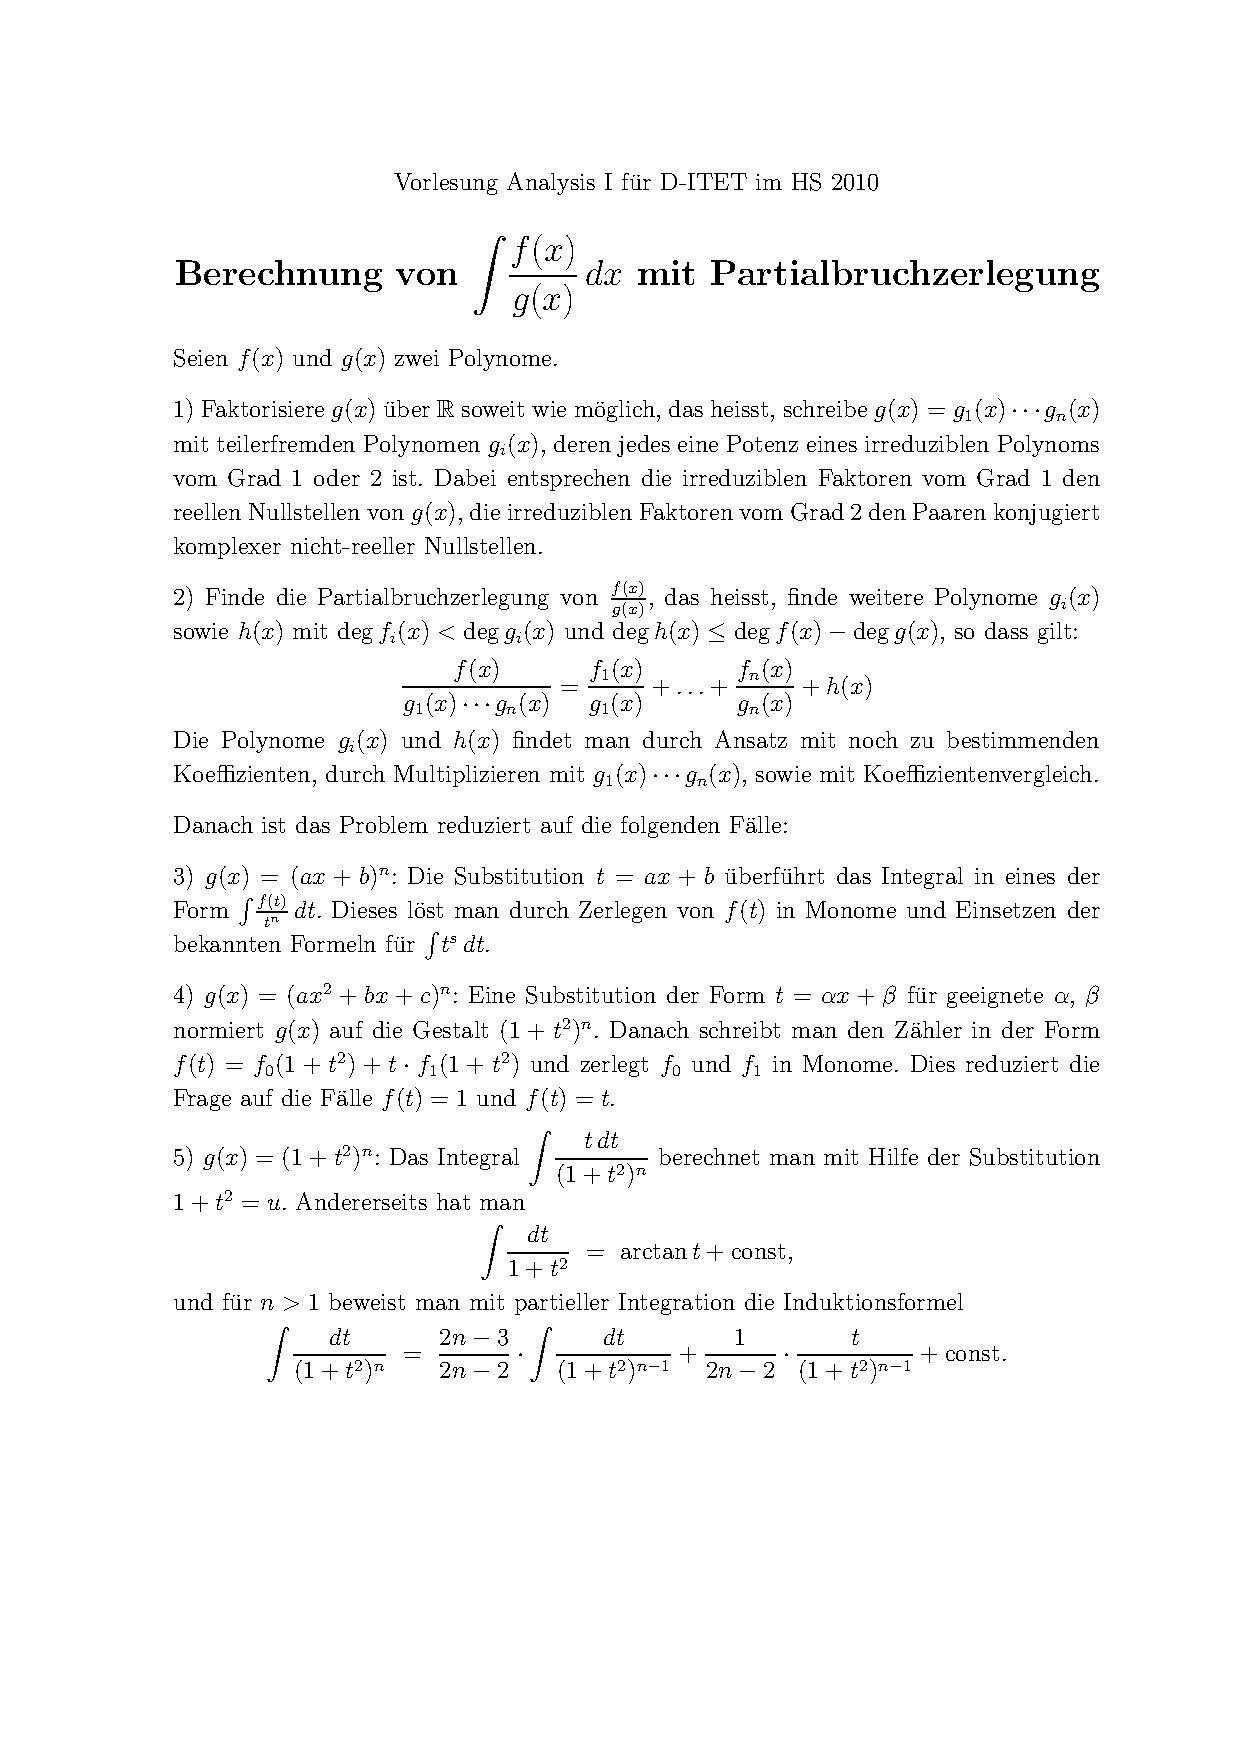
\includepdf[pages={1},addtotoc={1,section,1,Partialbruchzerlegung,newton}]{Partialbruchzerlegung}

\end{document}